
%!TEX root = ../main.tex
\addcontentsline{toc}{chapter}{LAMPIRAN}
\appendix

\chapter{Dokumentasi Source Code}

\begin{figure}[H]
  \centering{}
	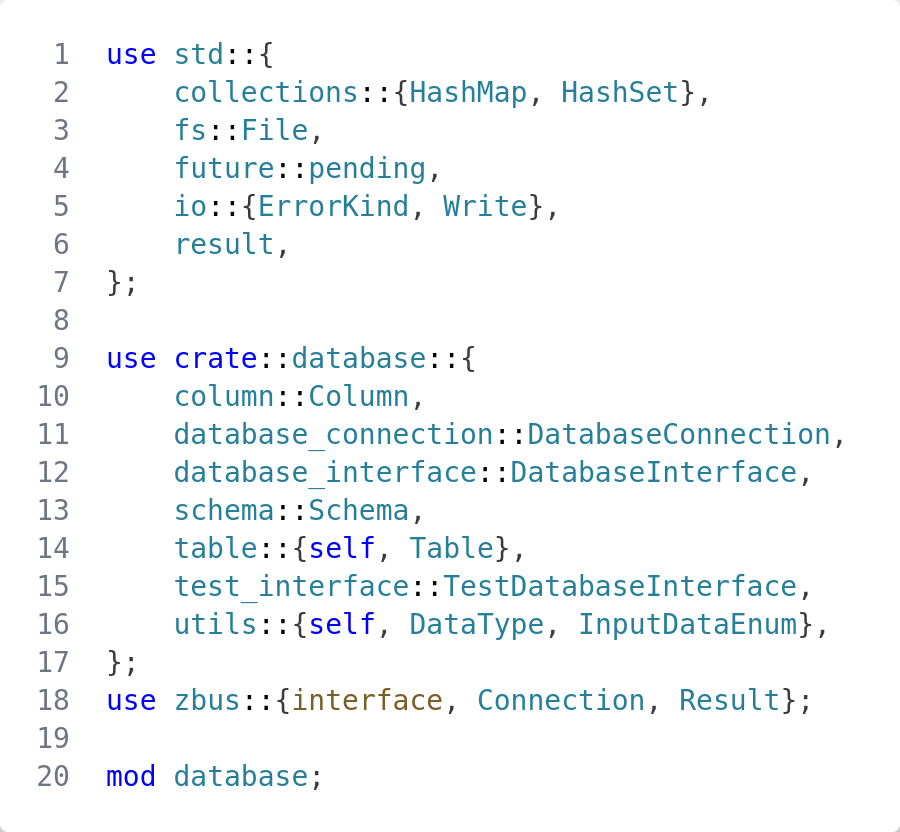
\includegraphics[width=0.9\textwidth]{gambar/lampiran/file-import-main.png}
  \caption{\emph{Import} dalam \emph{file} main.rs}
\end{figure}

\begin{figure}[H]
  \centering{}
	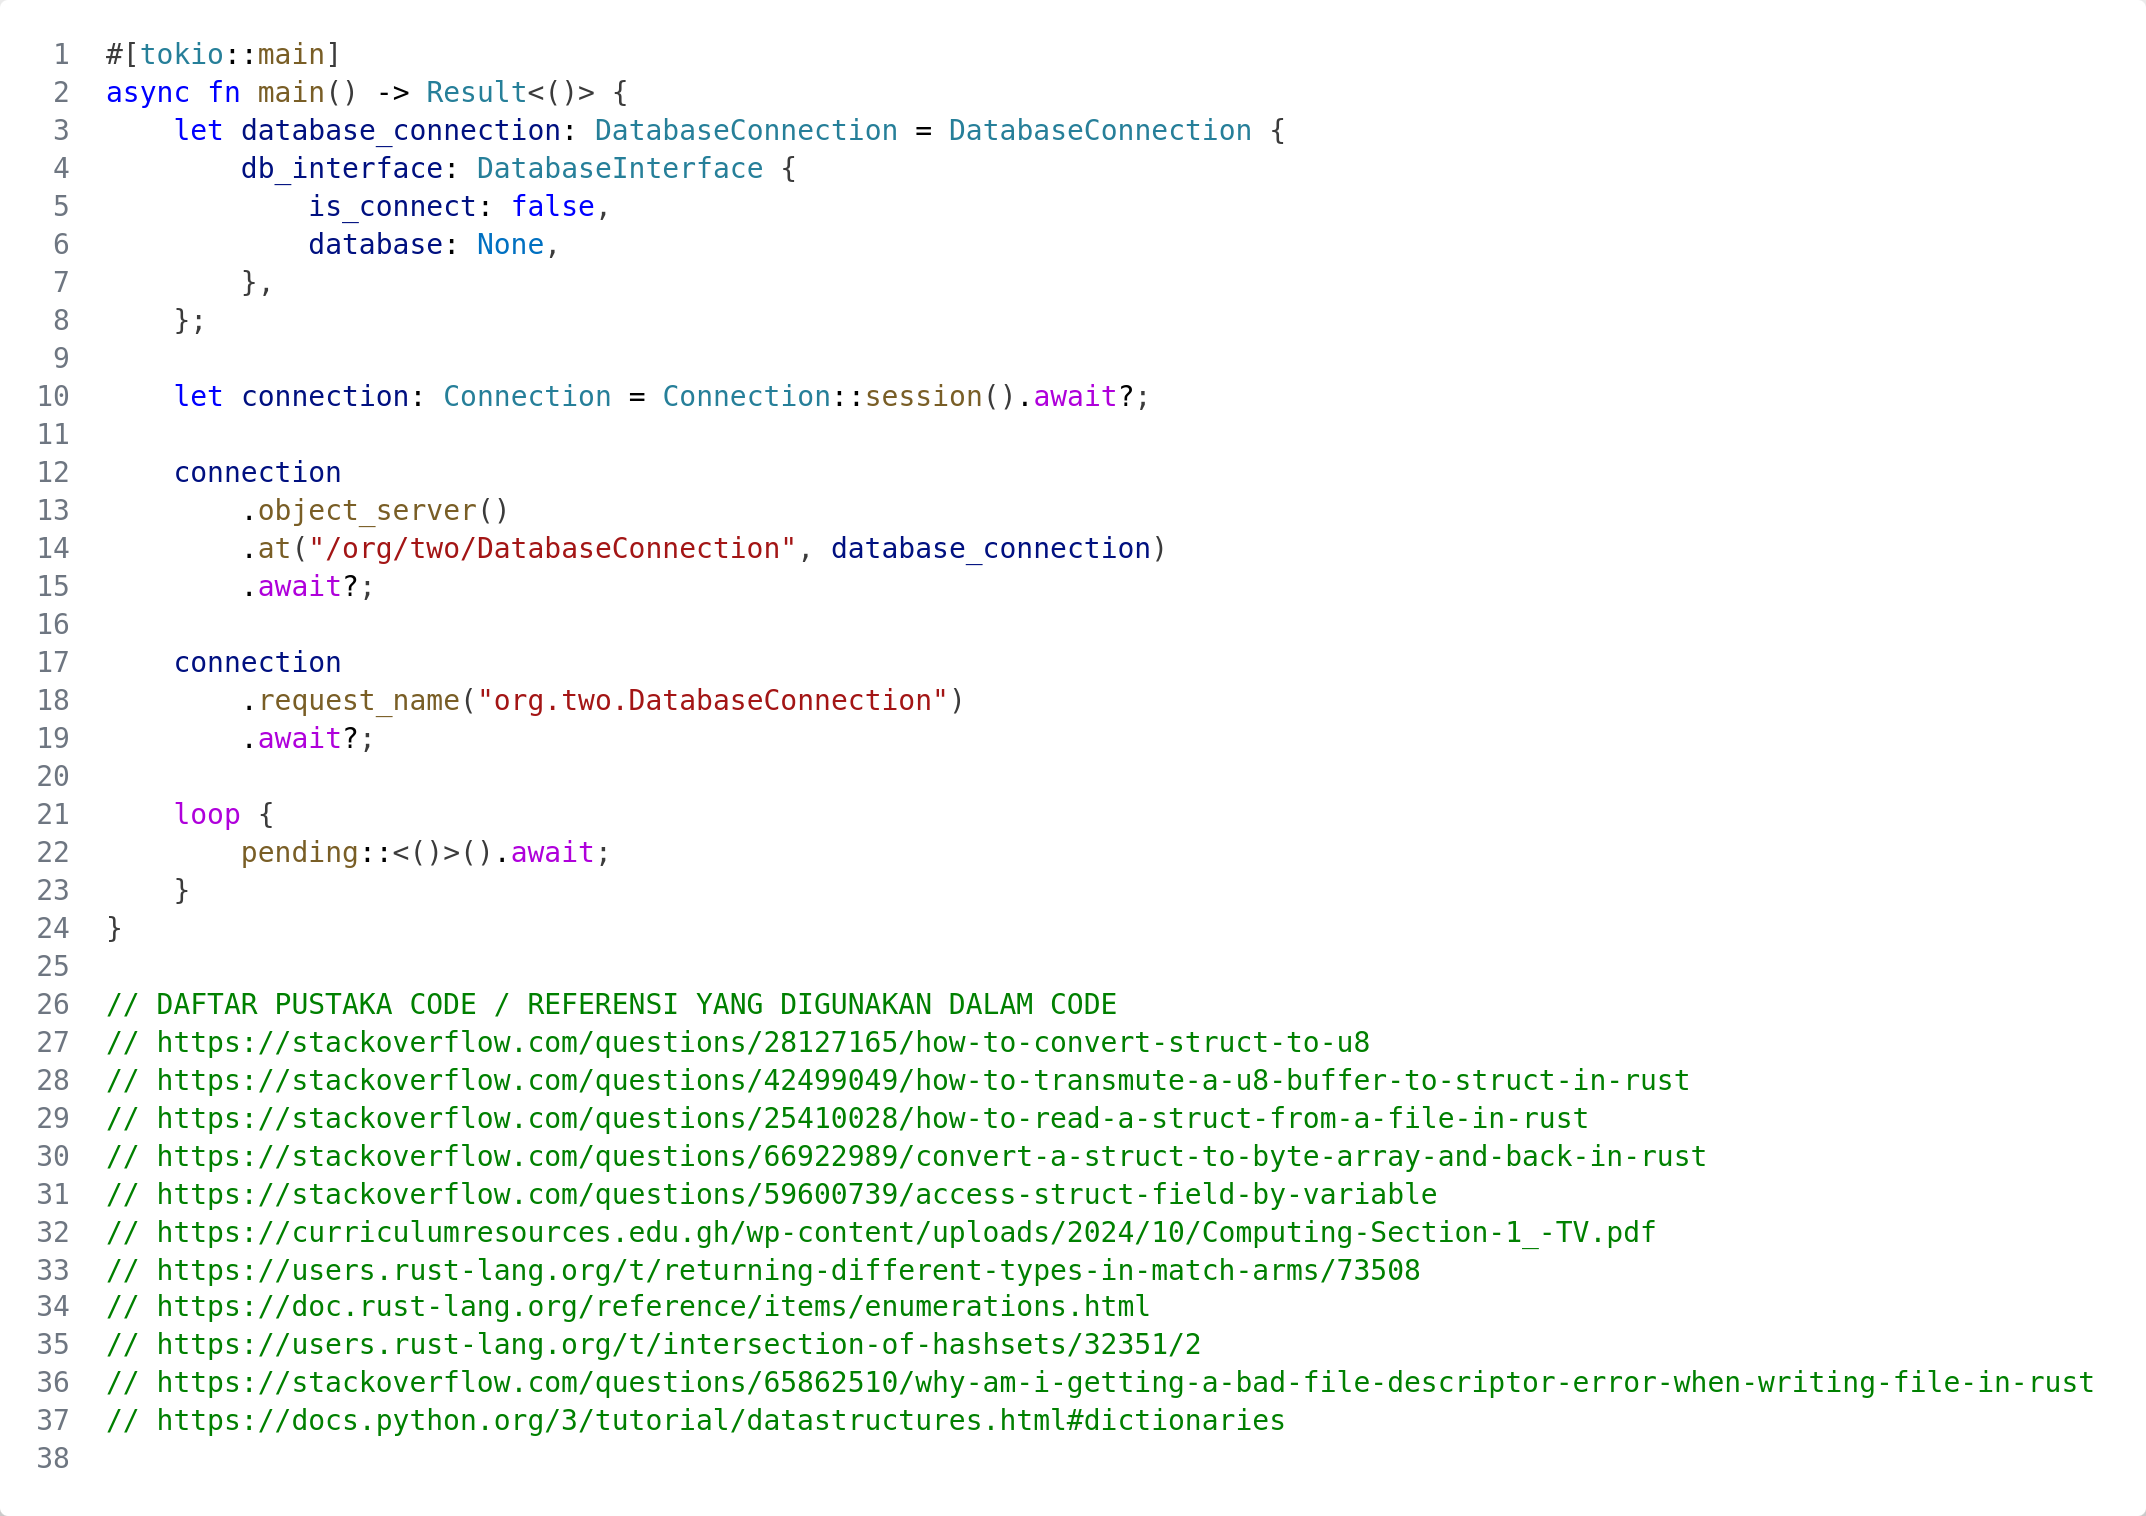
\includegraphics[width=0.9\textwidth]{gambar/lampiran/file-main-function.png}
  \caption{\emph{Function} main dalam \emph{file} main.rs}
\end{figure}

\begin{figure}[H]
  \centering{}
	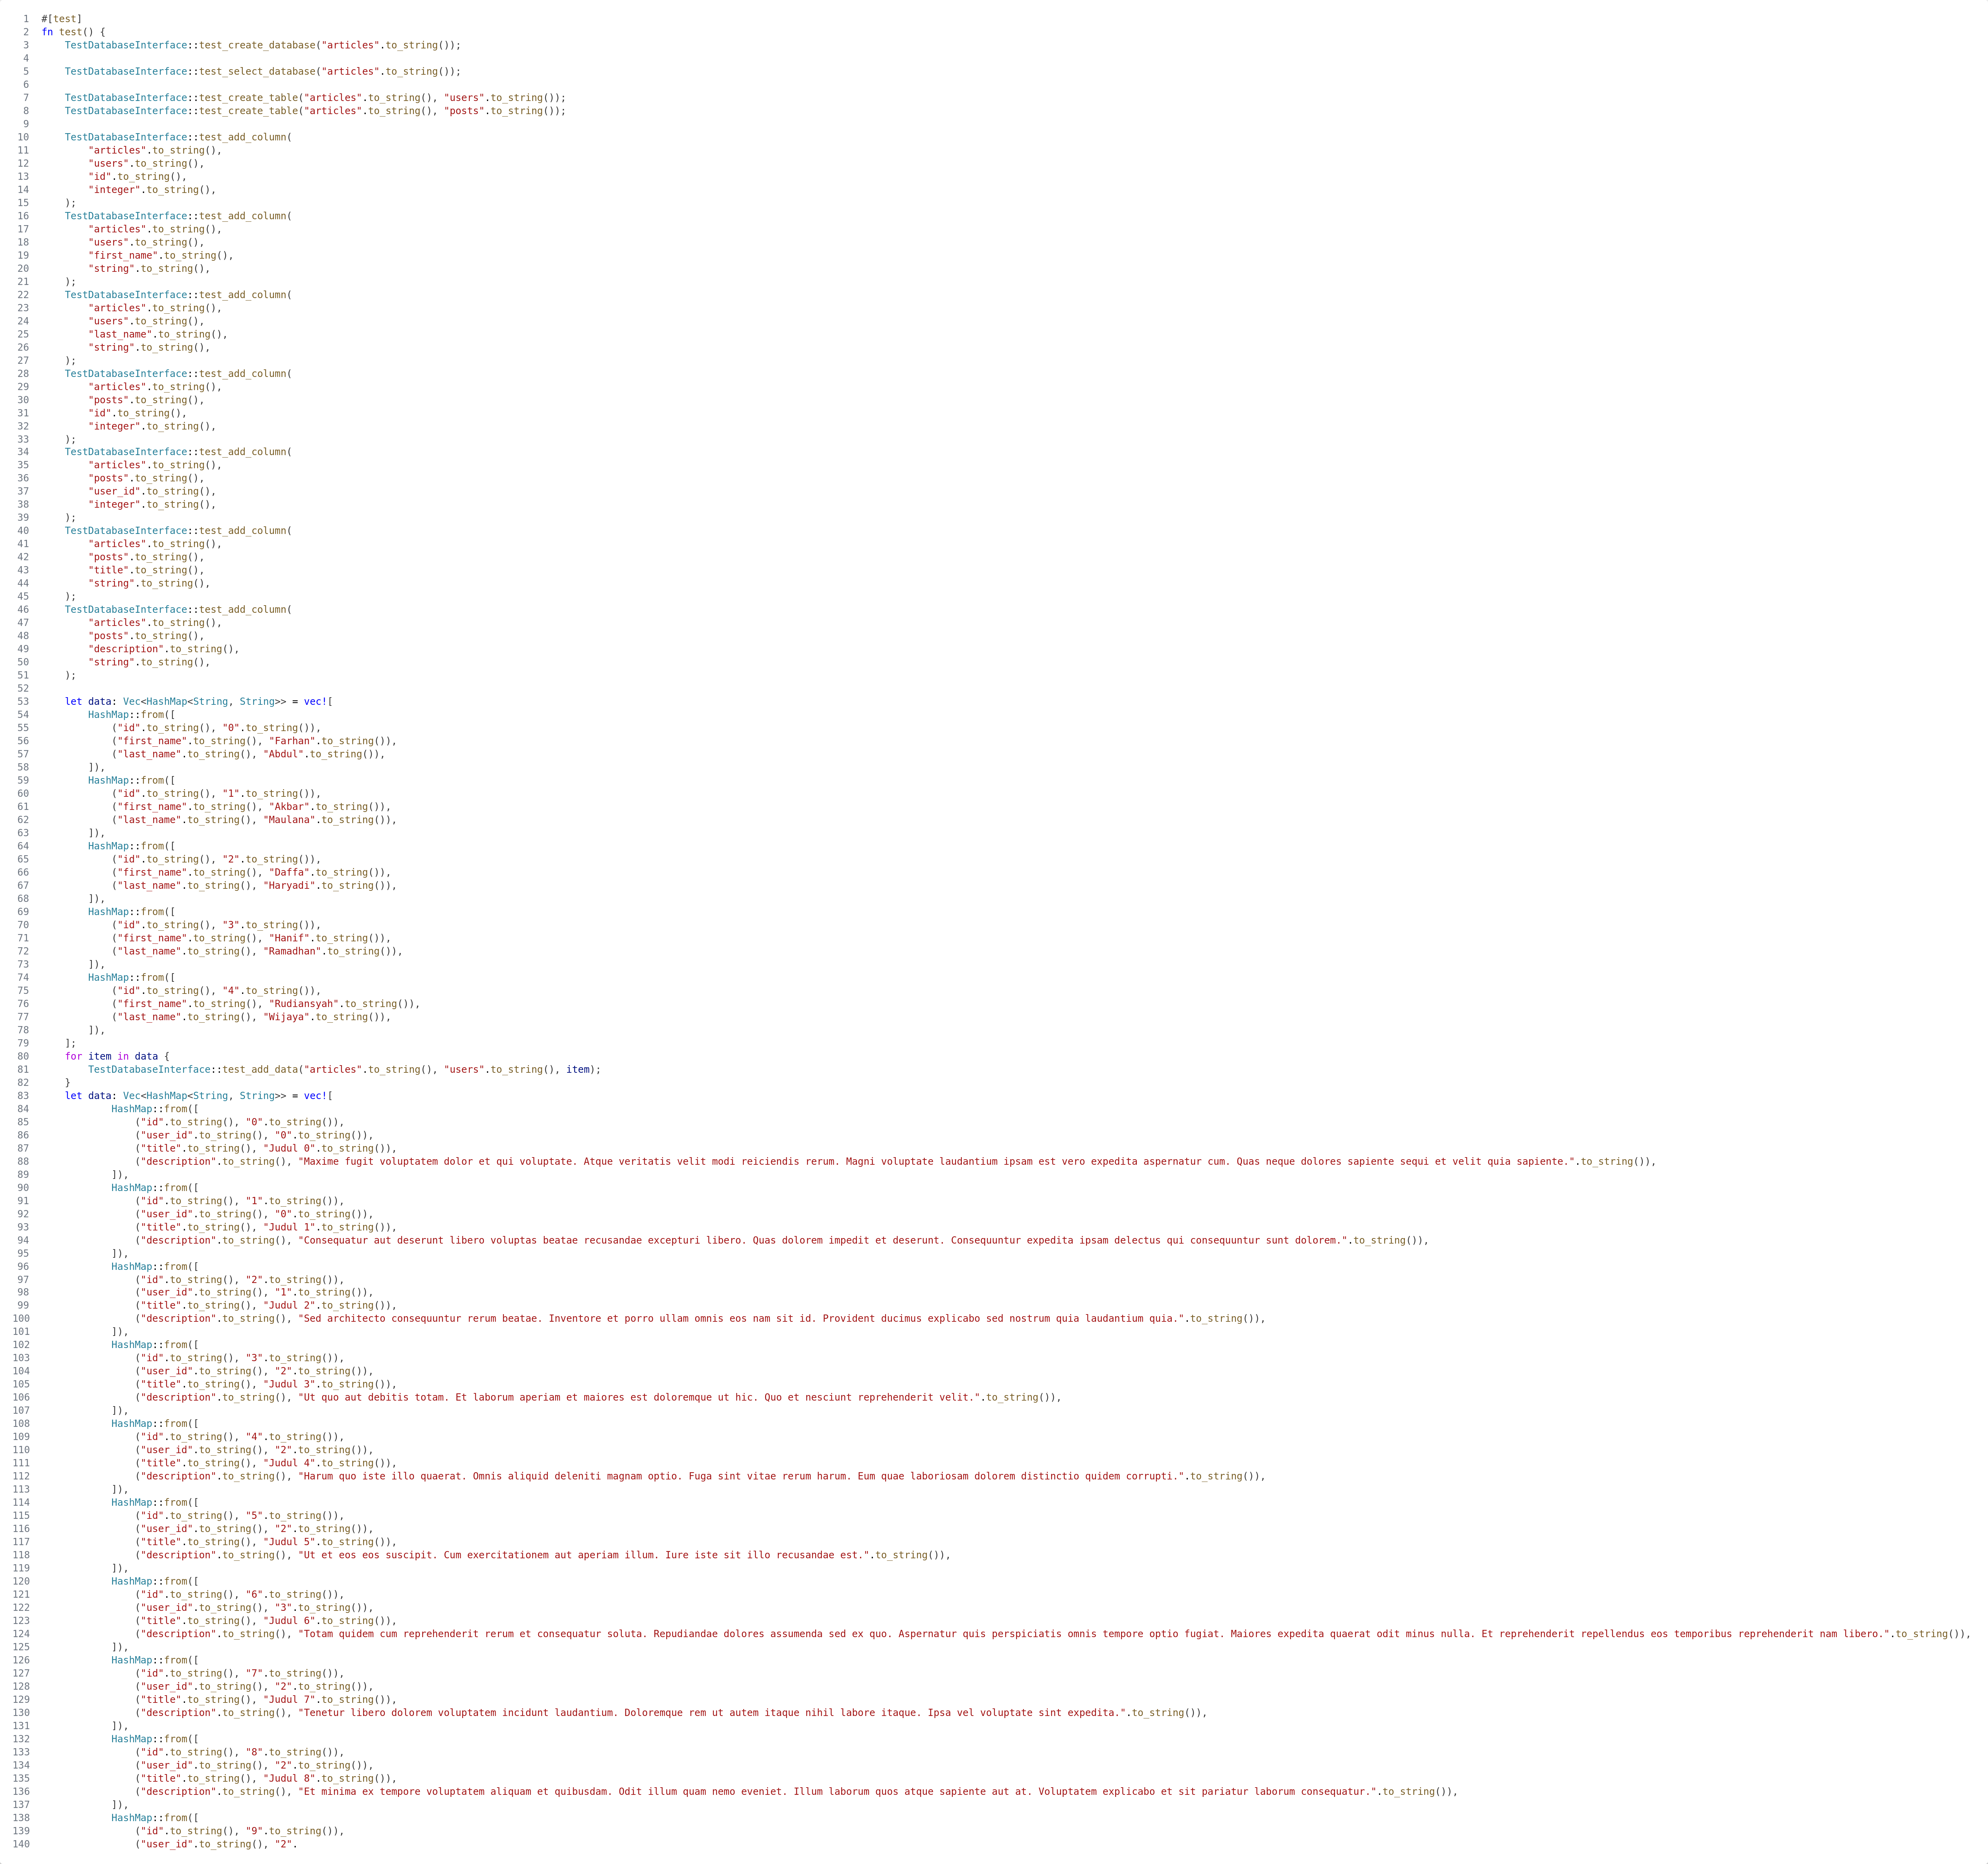
\includegraphics[width=0.9\textwidth]{gambar/lampiran/file-main-test-1.png}
  \caption{\emph{Function} test dalam \emph{file} main.rs bagian 1}
\end{figure}

\begin{figure}[H]
  \centering{}
	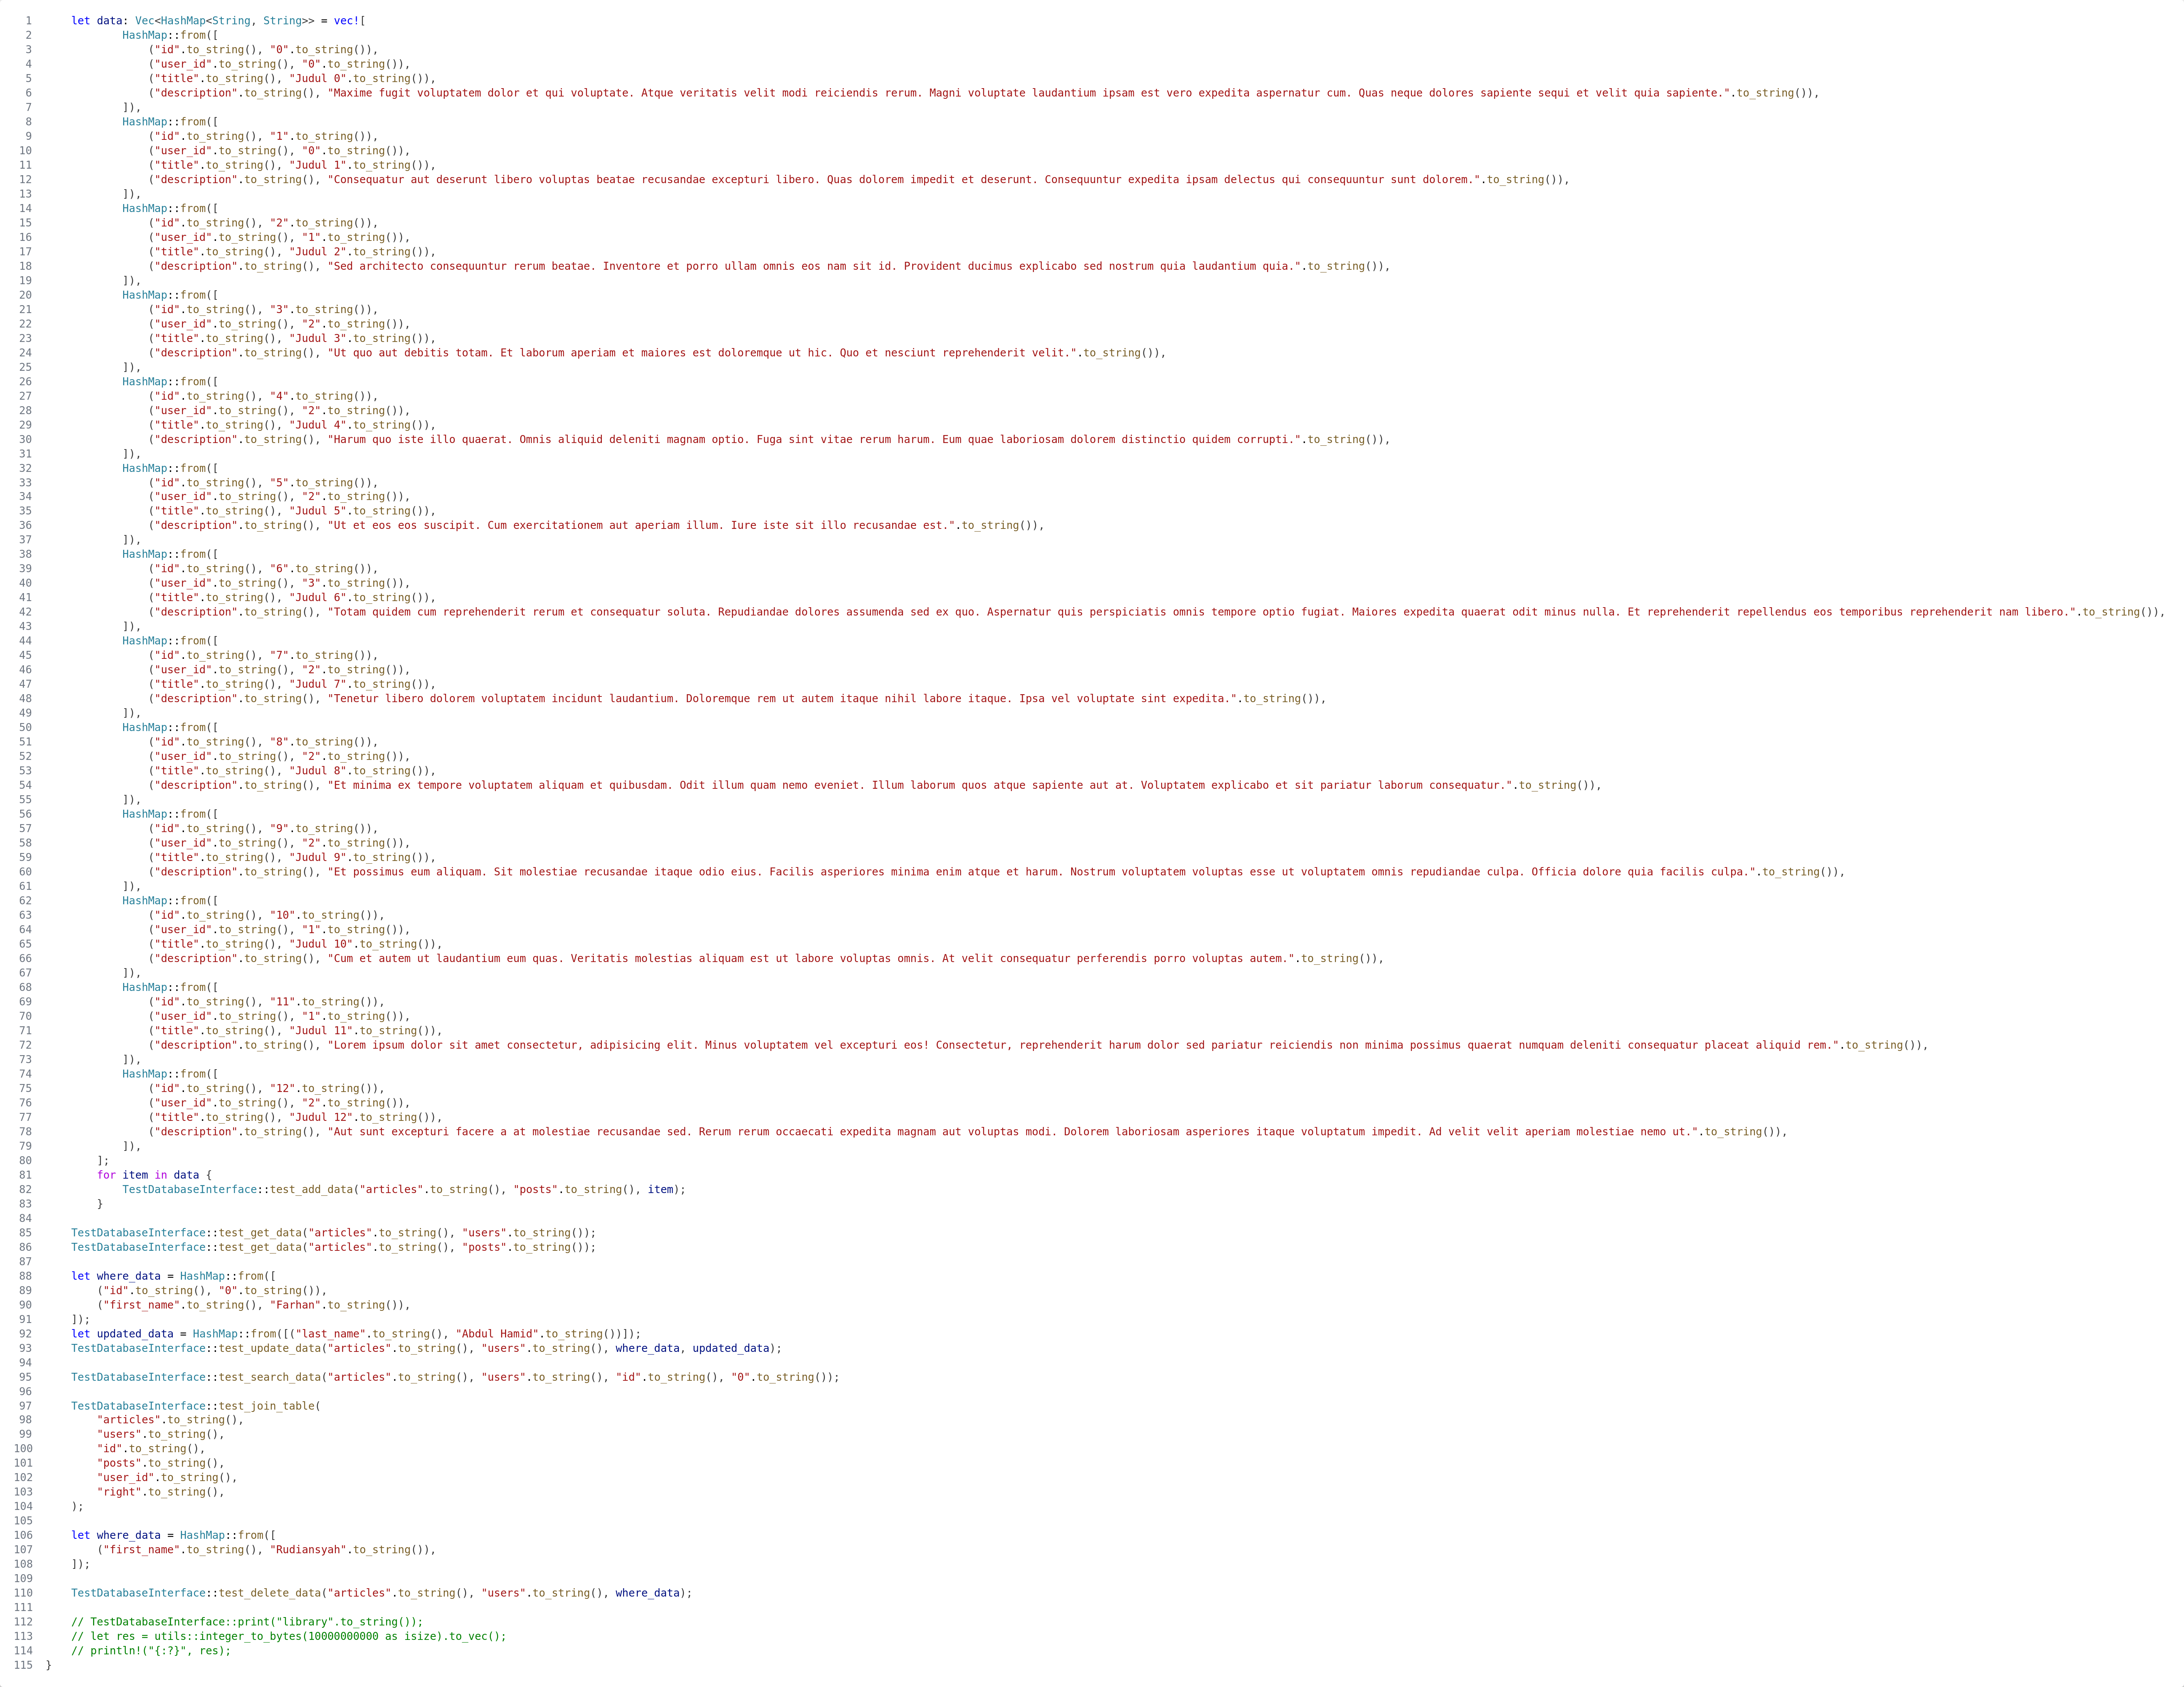
\includegraphics[width=0.9\textwidth]{gambar/lampiran/file-main-test-2.png}
  \caption{\emph{Function} test dalam \emph{file} main.rs bagian 2}
\end{figure}

\begin{figure}[H]
  \centering{}
	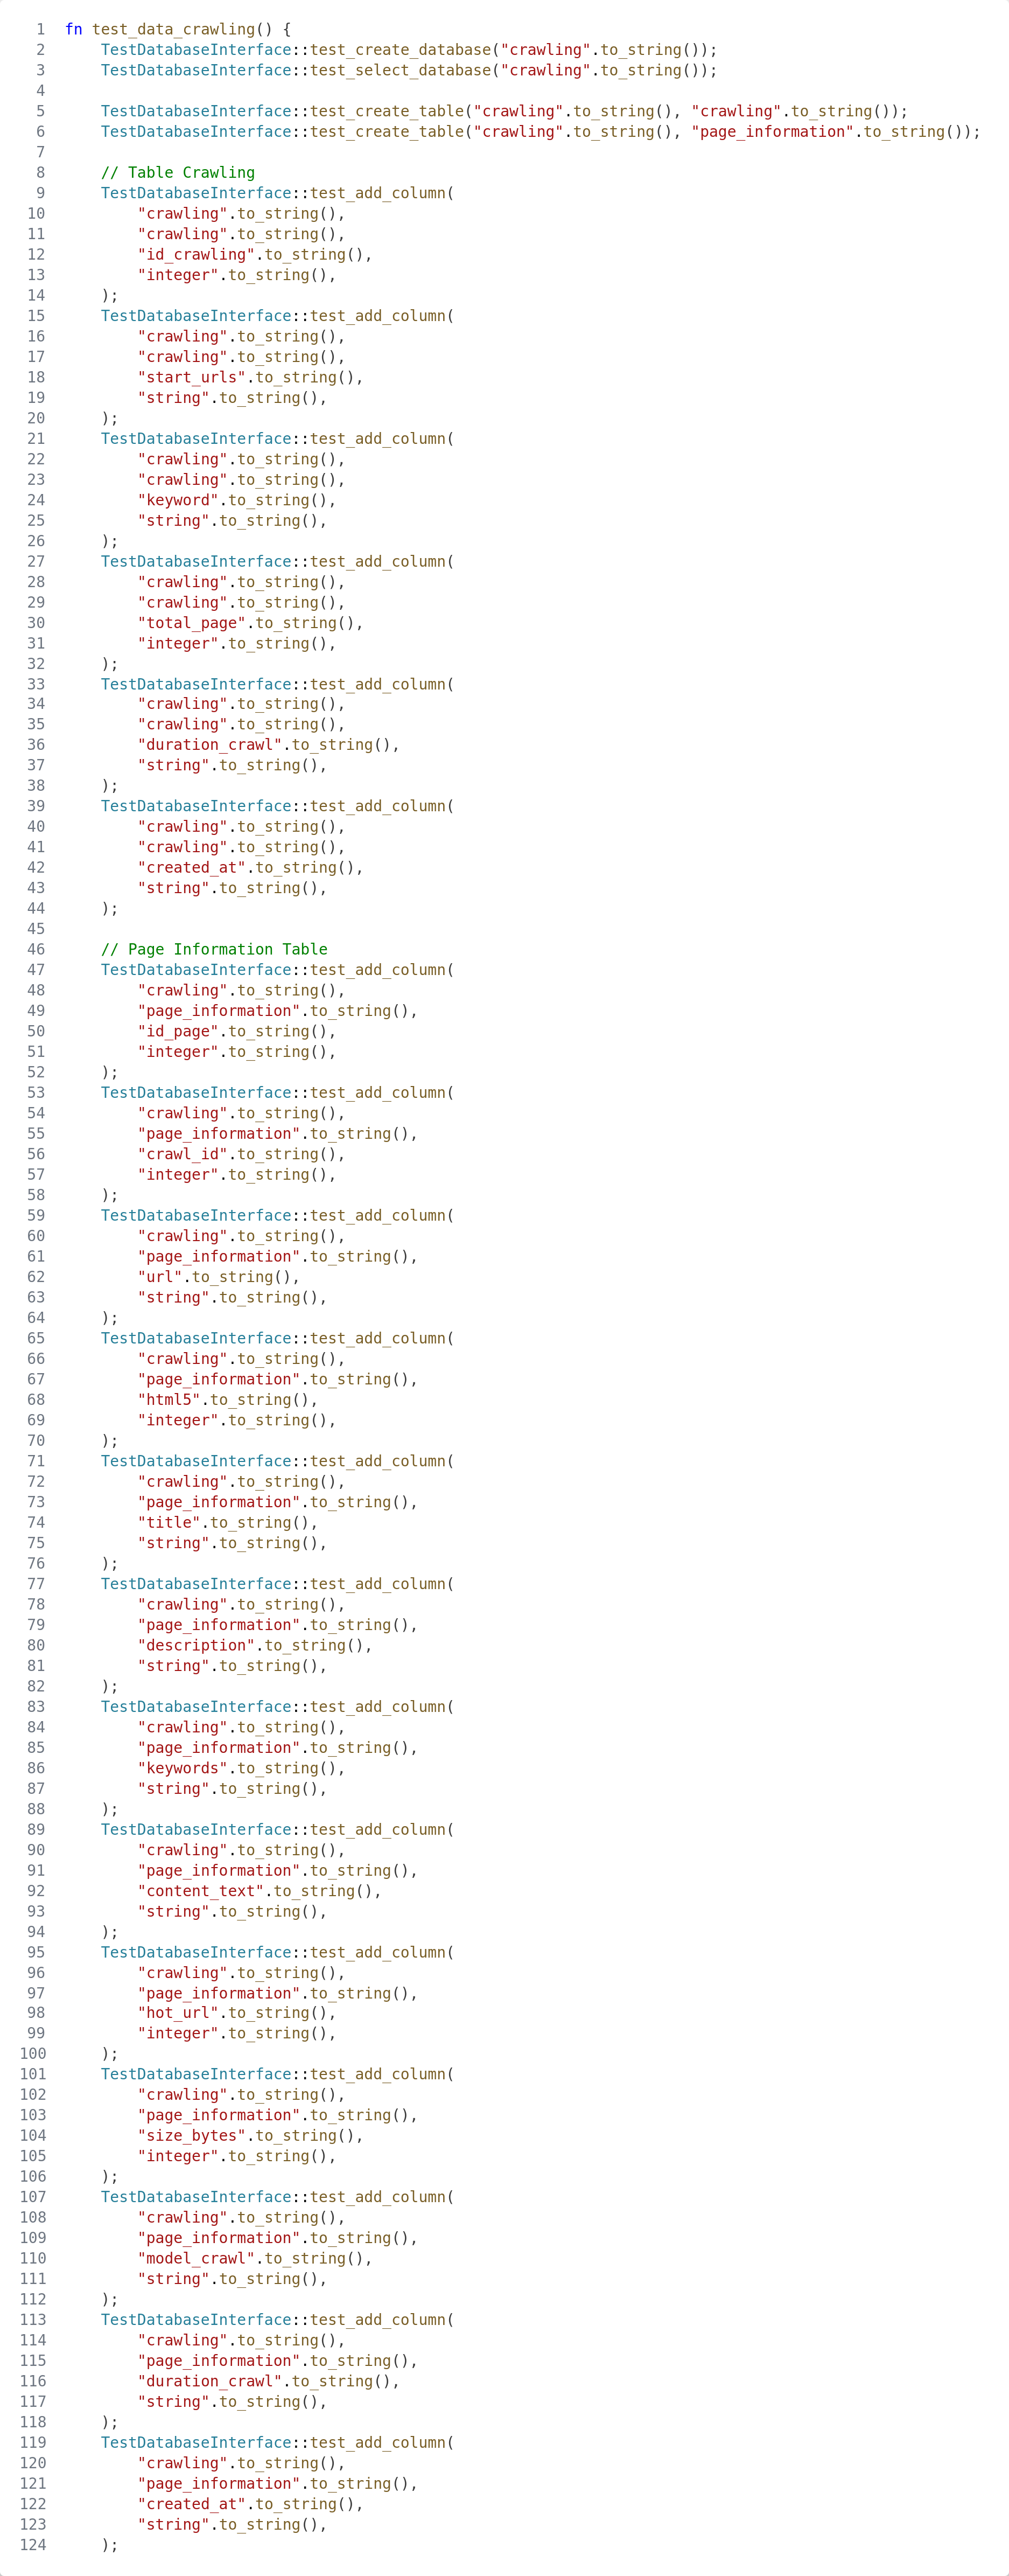
\includegraphics[width=0.4\textwidth]{gambar/lampiran/file-main-test-data-1.png}
  \caption{\emph{Function} test\_data\_crawling dalam \emph{file} main.rs. Keseluruhan \emph{function} dapat dilihat di \emph{source code} langsung}
\end{figure}


\begin{figure}[H]
  \centering{}
	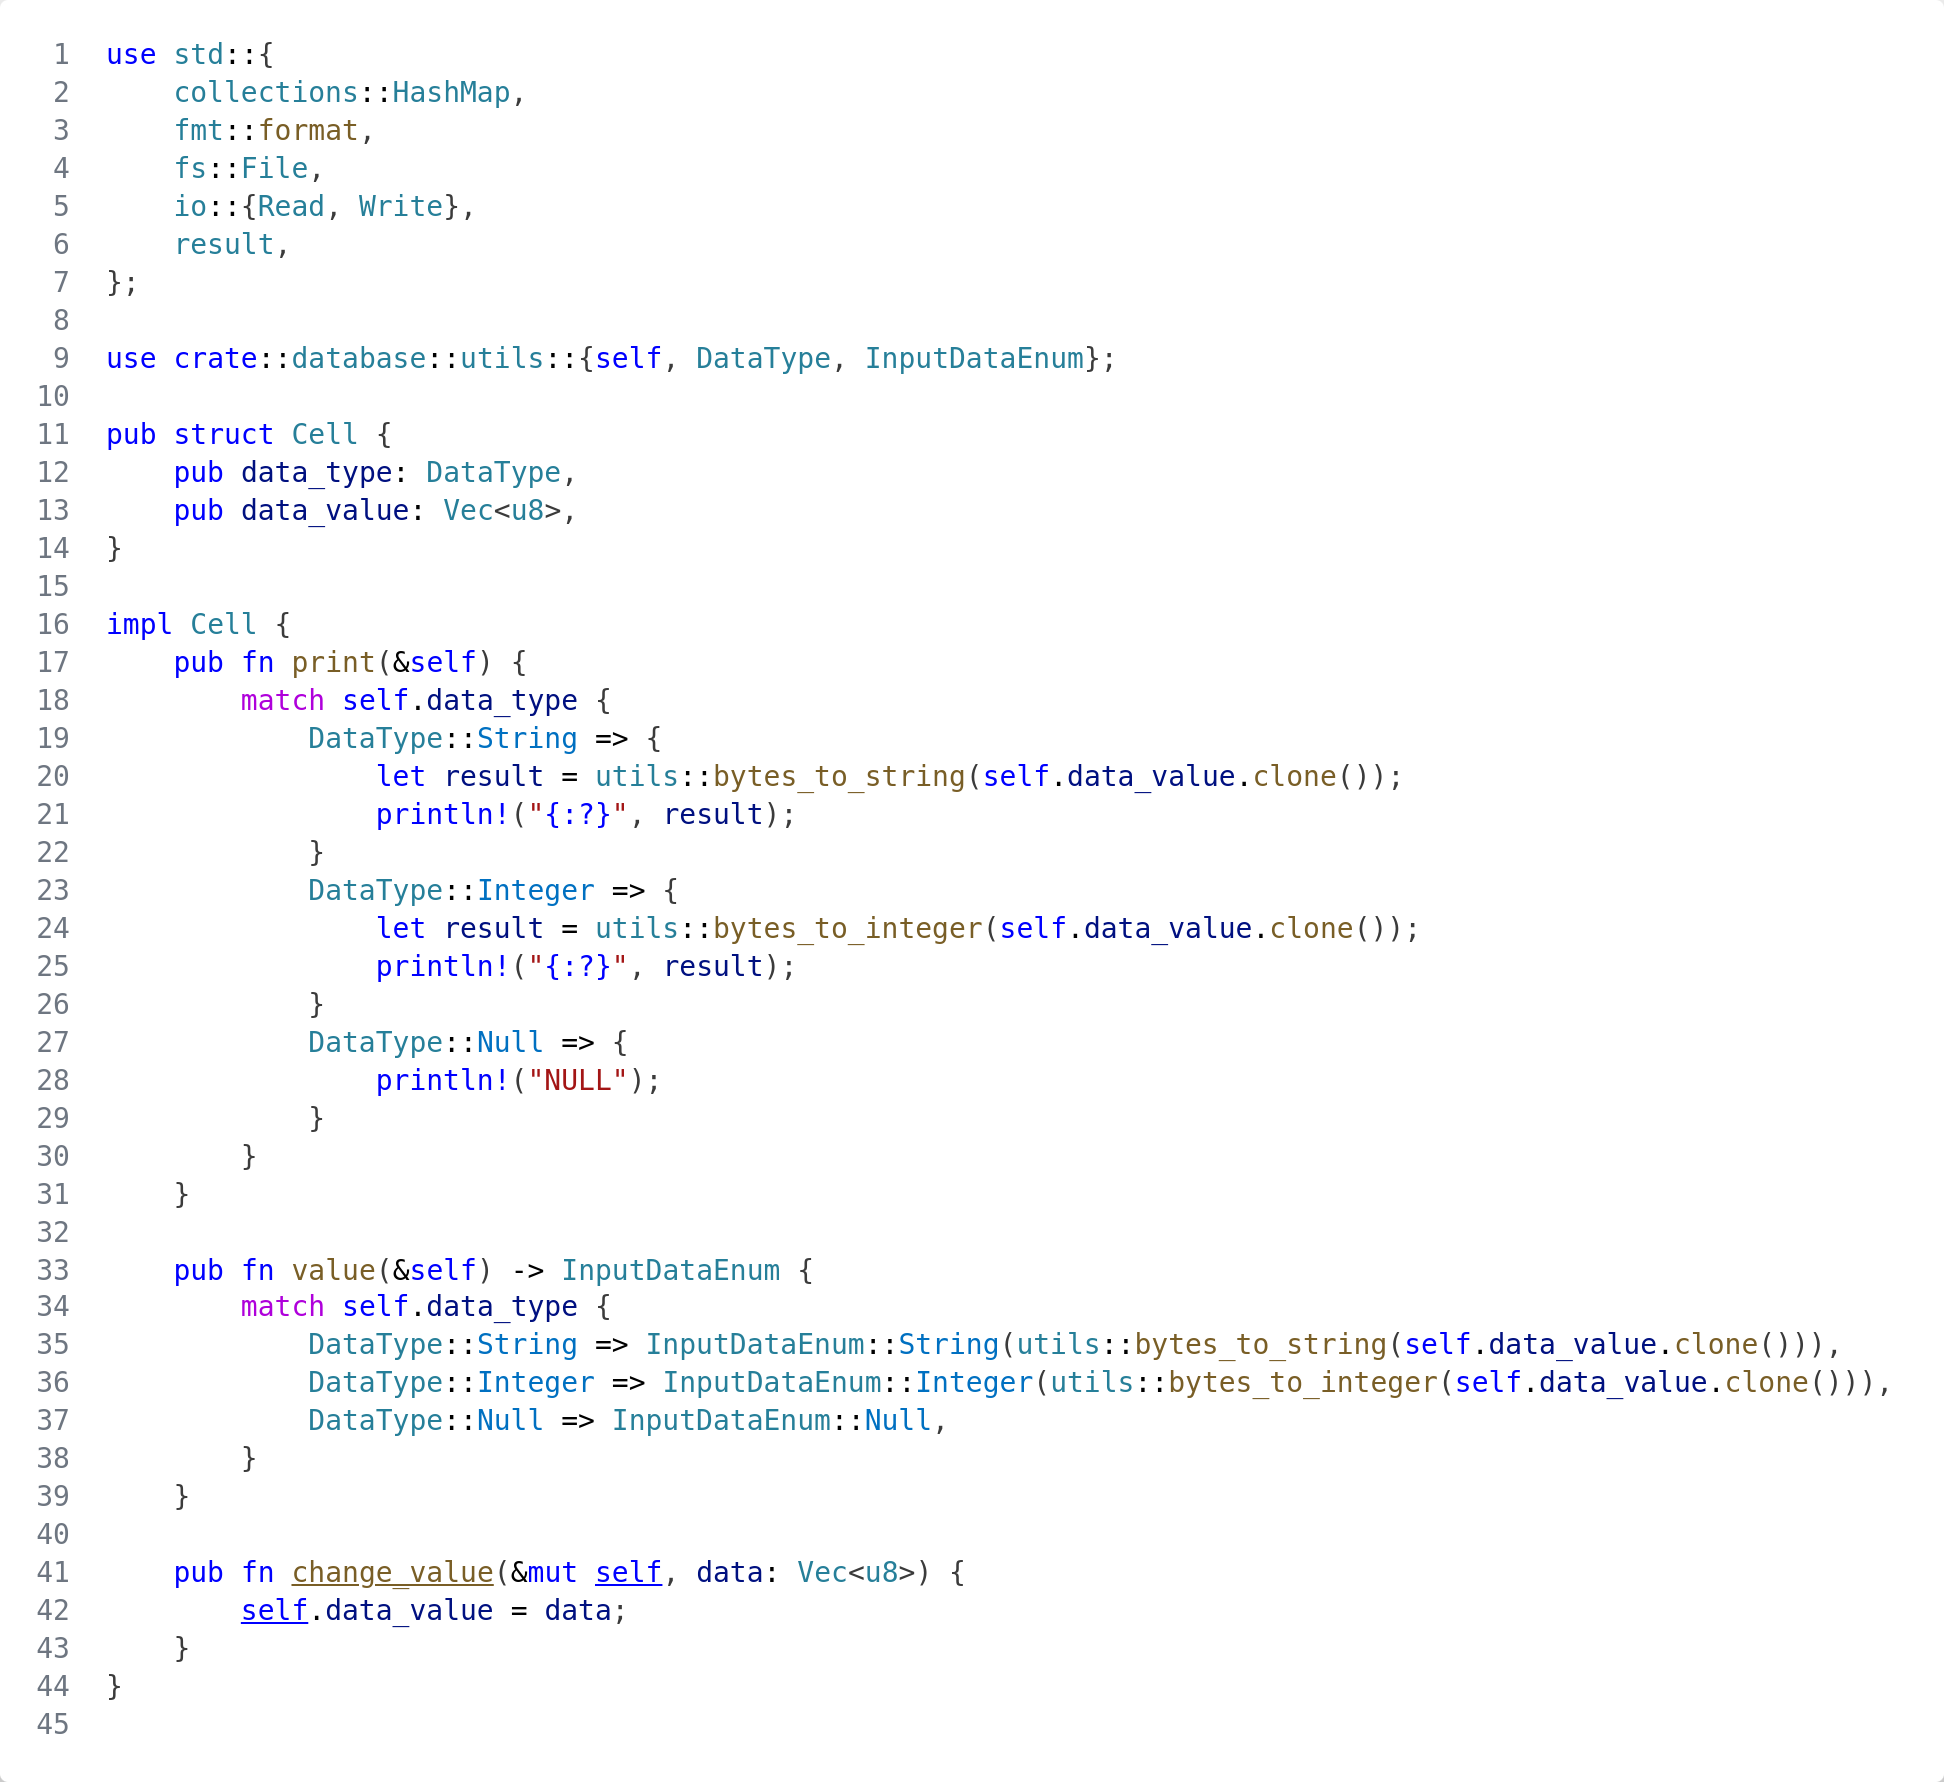
\includegraphics[width=0.9\textwidth]{gambar/lampiran/file-cell.png}
  \caption{\emph{File} cell.rs}
\end{figure}

\begin{figure}[H]
  \centering{}
	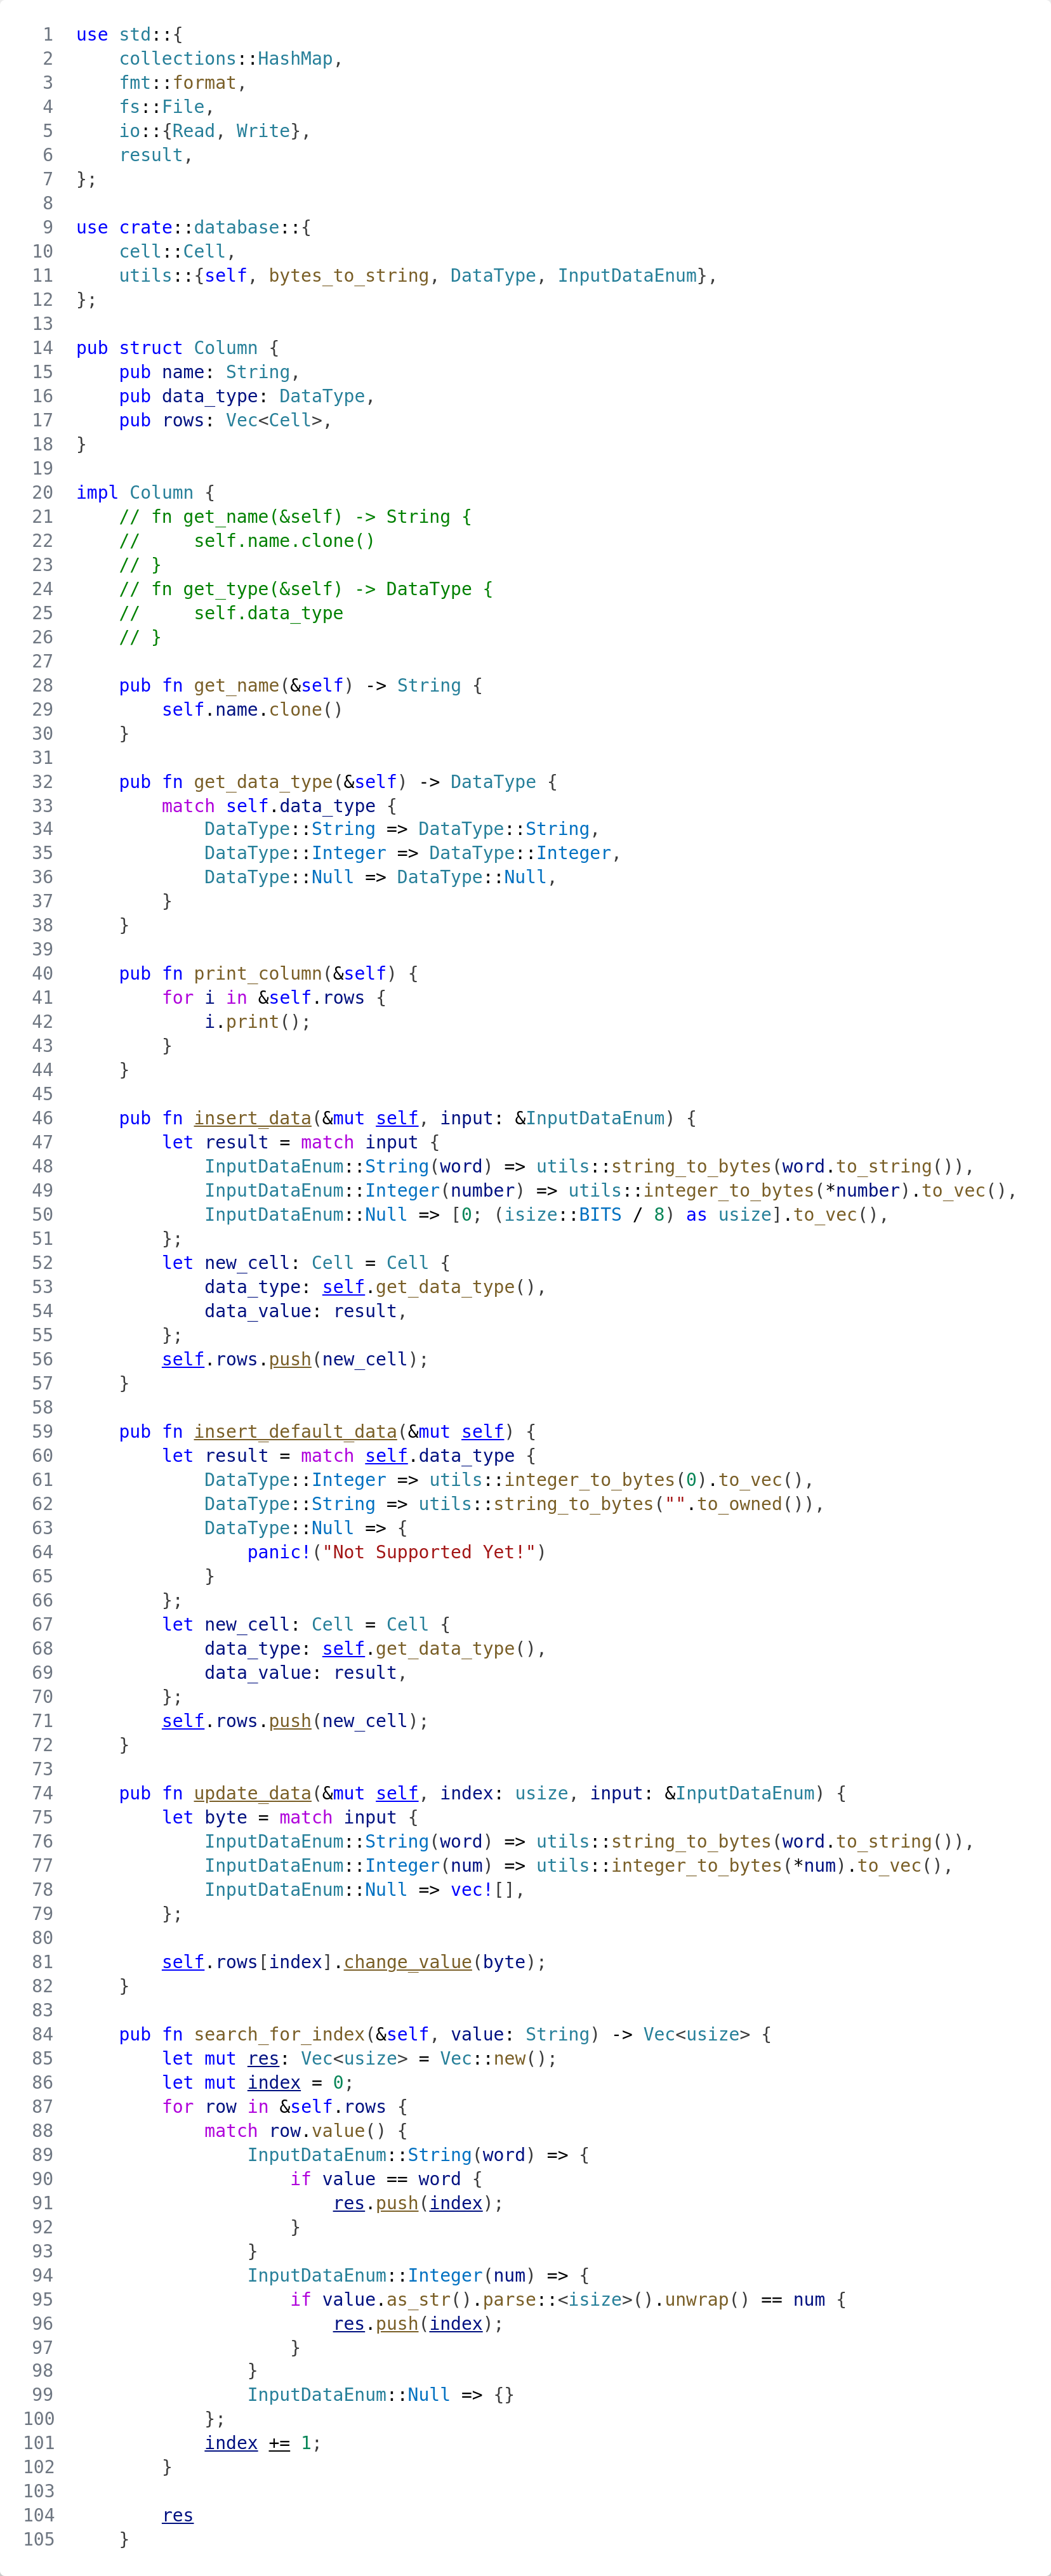
\includegraphics[width=0.6\textwidth]{gambar/lampiran/file-column-1.png}
  \caption{\emph{File} column.rs bagian 1}
\end{figure}

\begin{figure}[H]
  \centering{}
	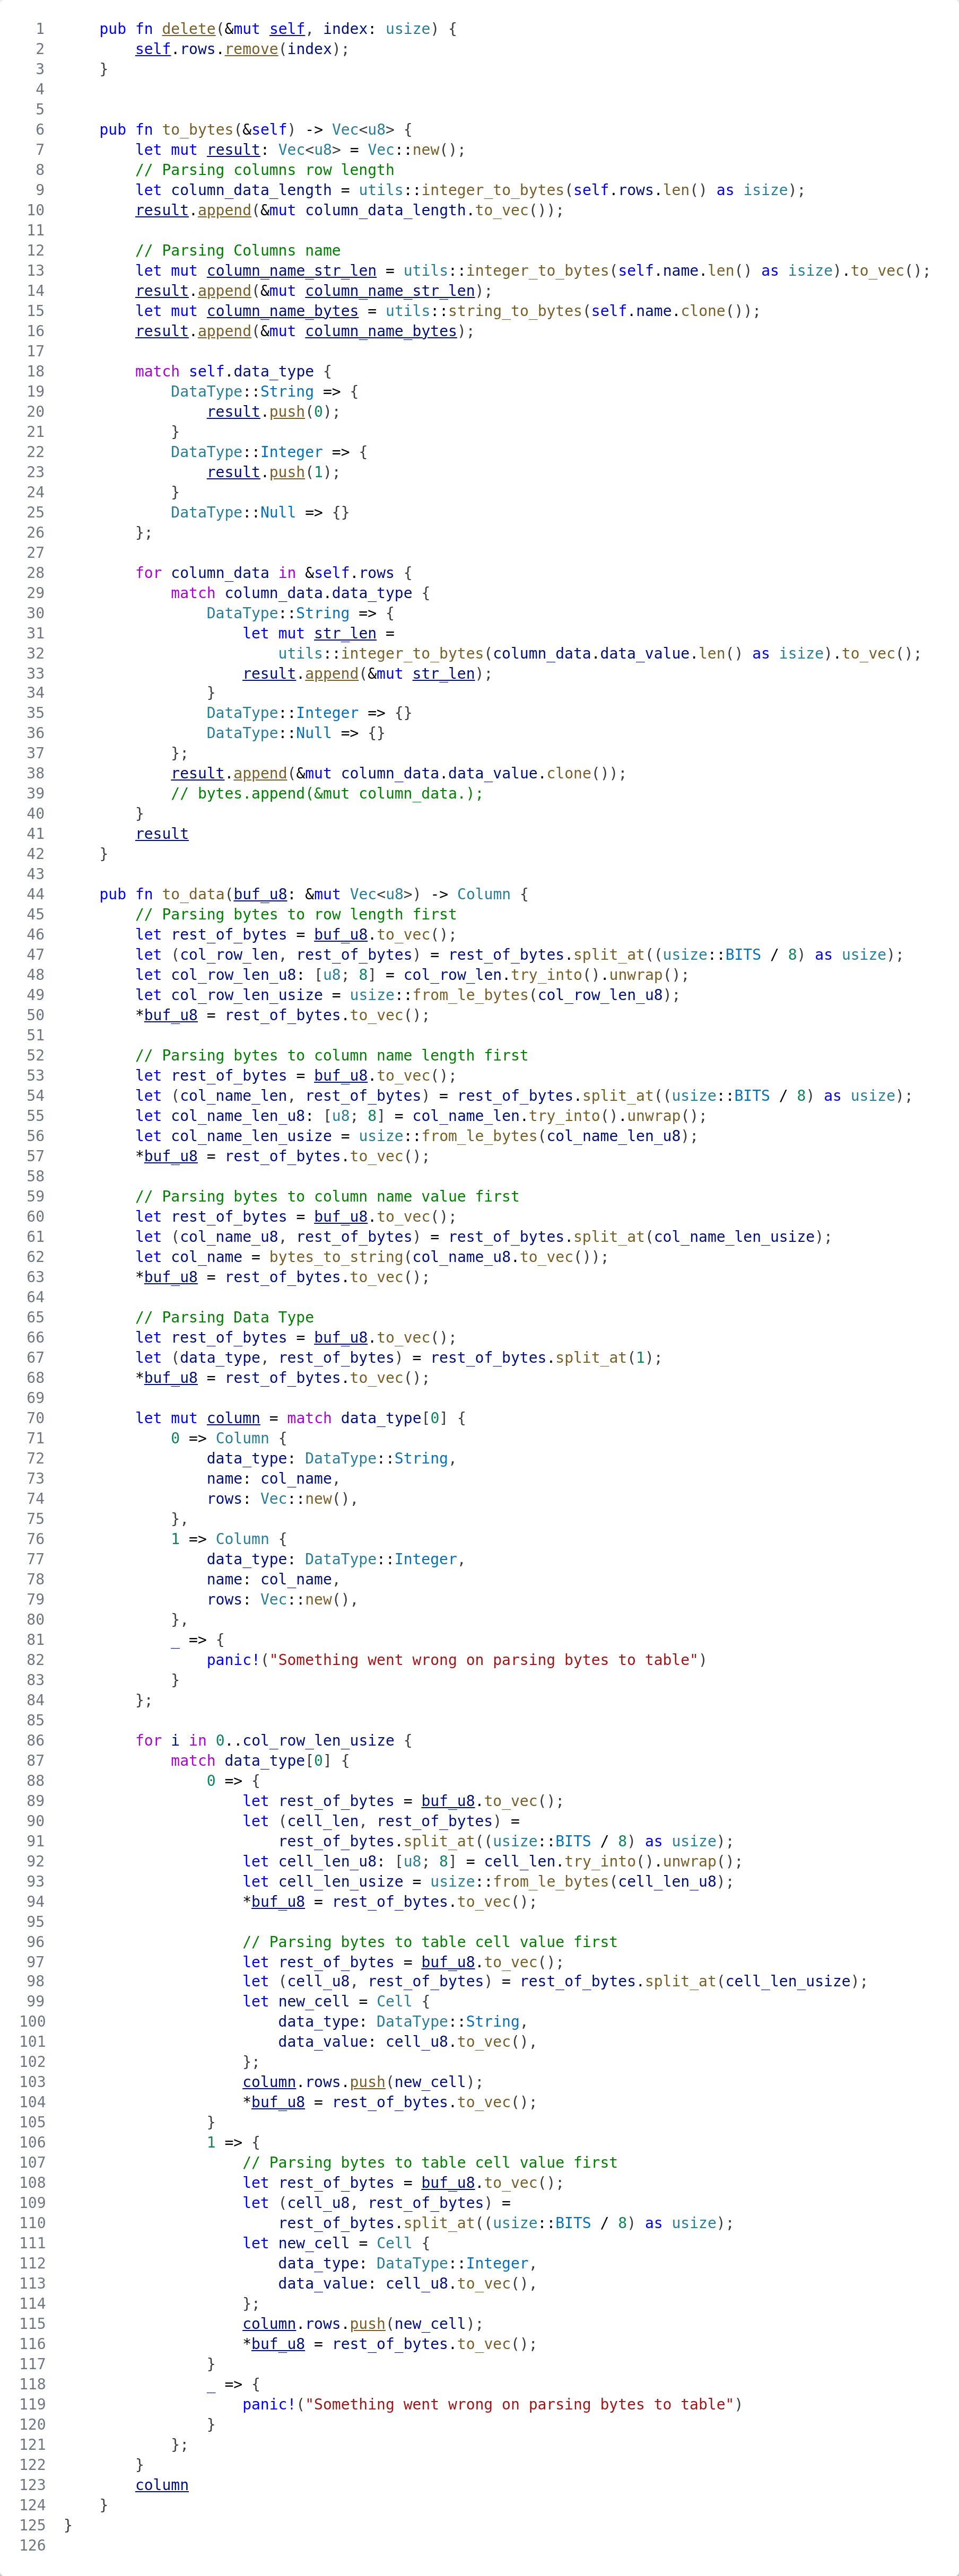
\includegraphics[width=0.4\textwidth]{gambar/lampiran/file-column-2.png}
  \caption{\emph{File} column.rs bagian 2}
\end{figure}

\begin{figure}[H]
  \centering{}
	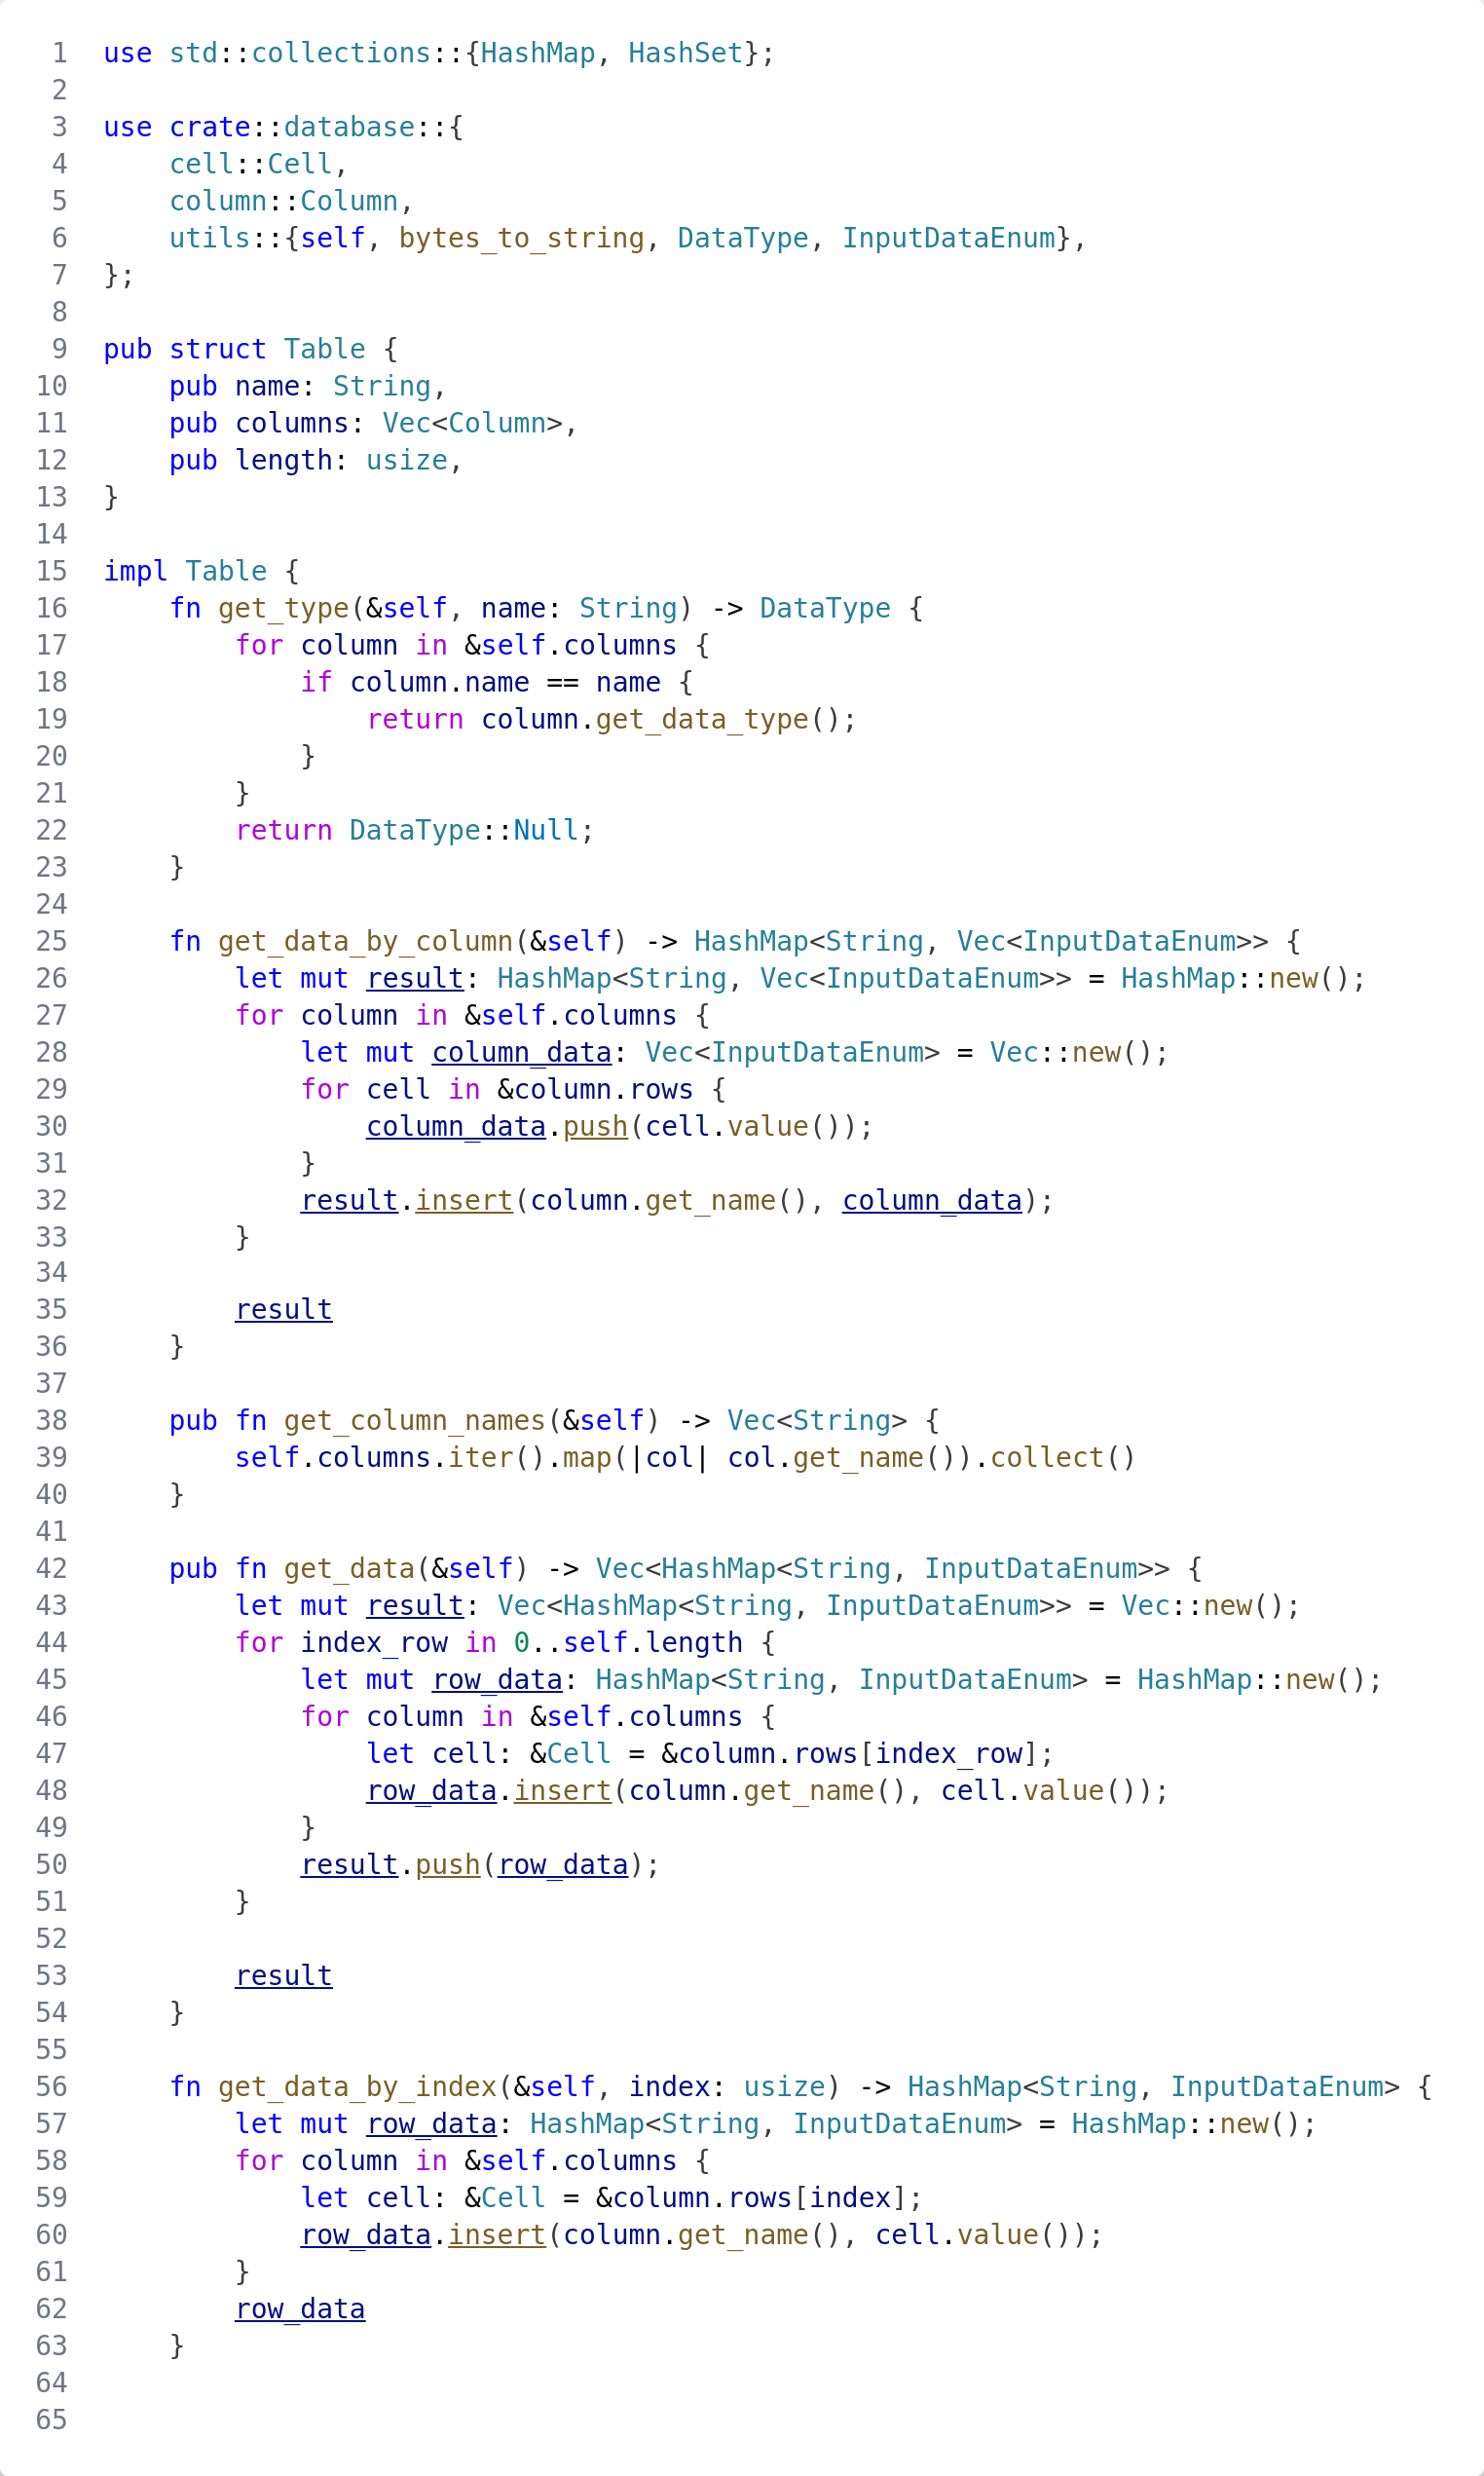
\includegraphics[width=0.7\textwidth]{gambar/lampiran/file-table-1.png}
  \caption{\emph{File} table.rs bagian 1}
\end{figure}

\begin{figure}[H]
  \centering{}
	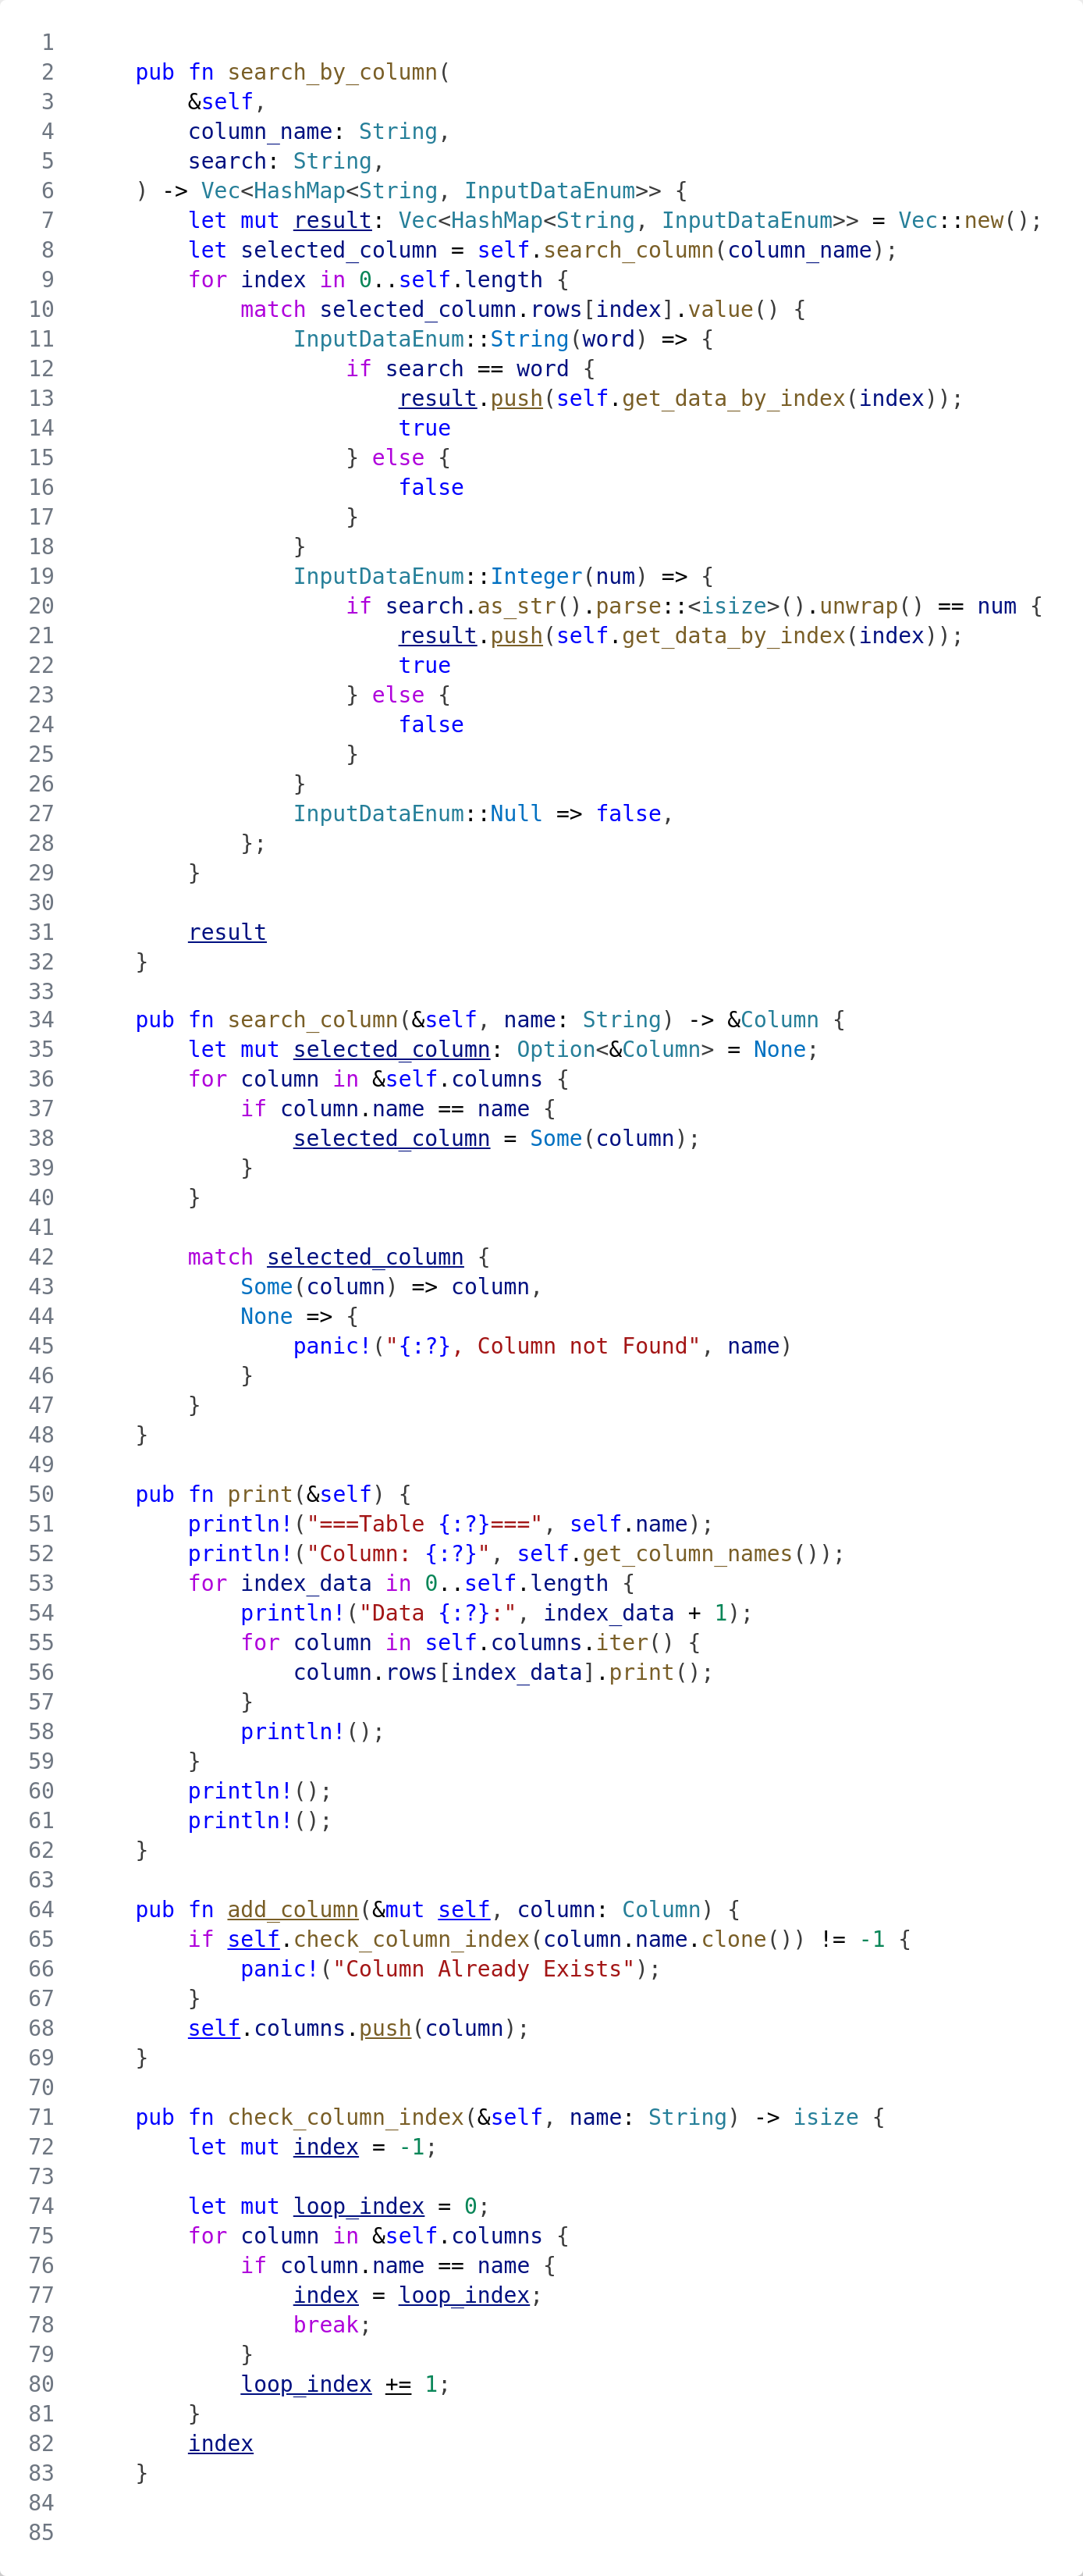
\includegraphics[width=0.6\textwidth]{gambar/lampiran/file-table-2.png}
  \caption{\emph{File} table.rs bagian 2}
\end{figure}

\begin{figure}[H]
  \centering{}
	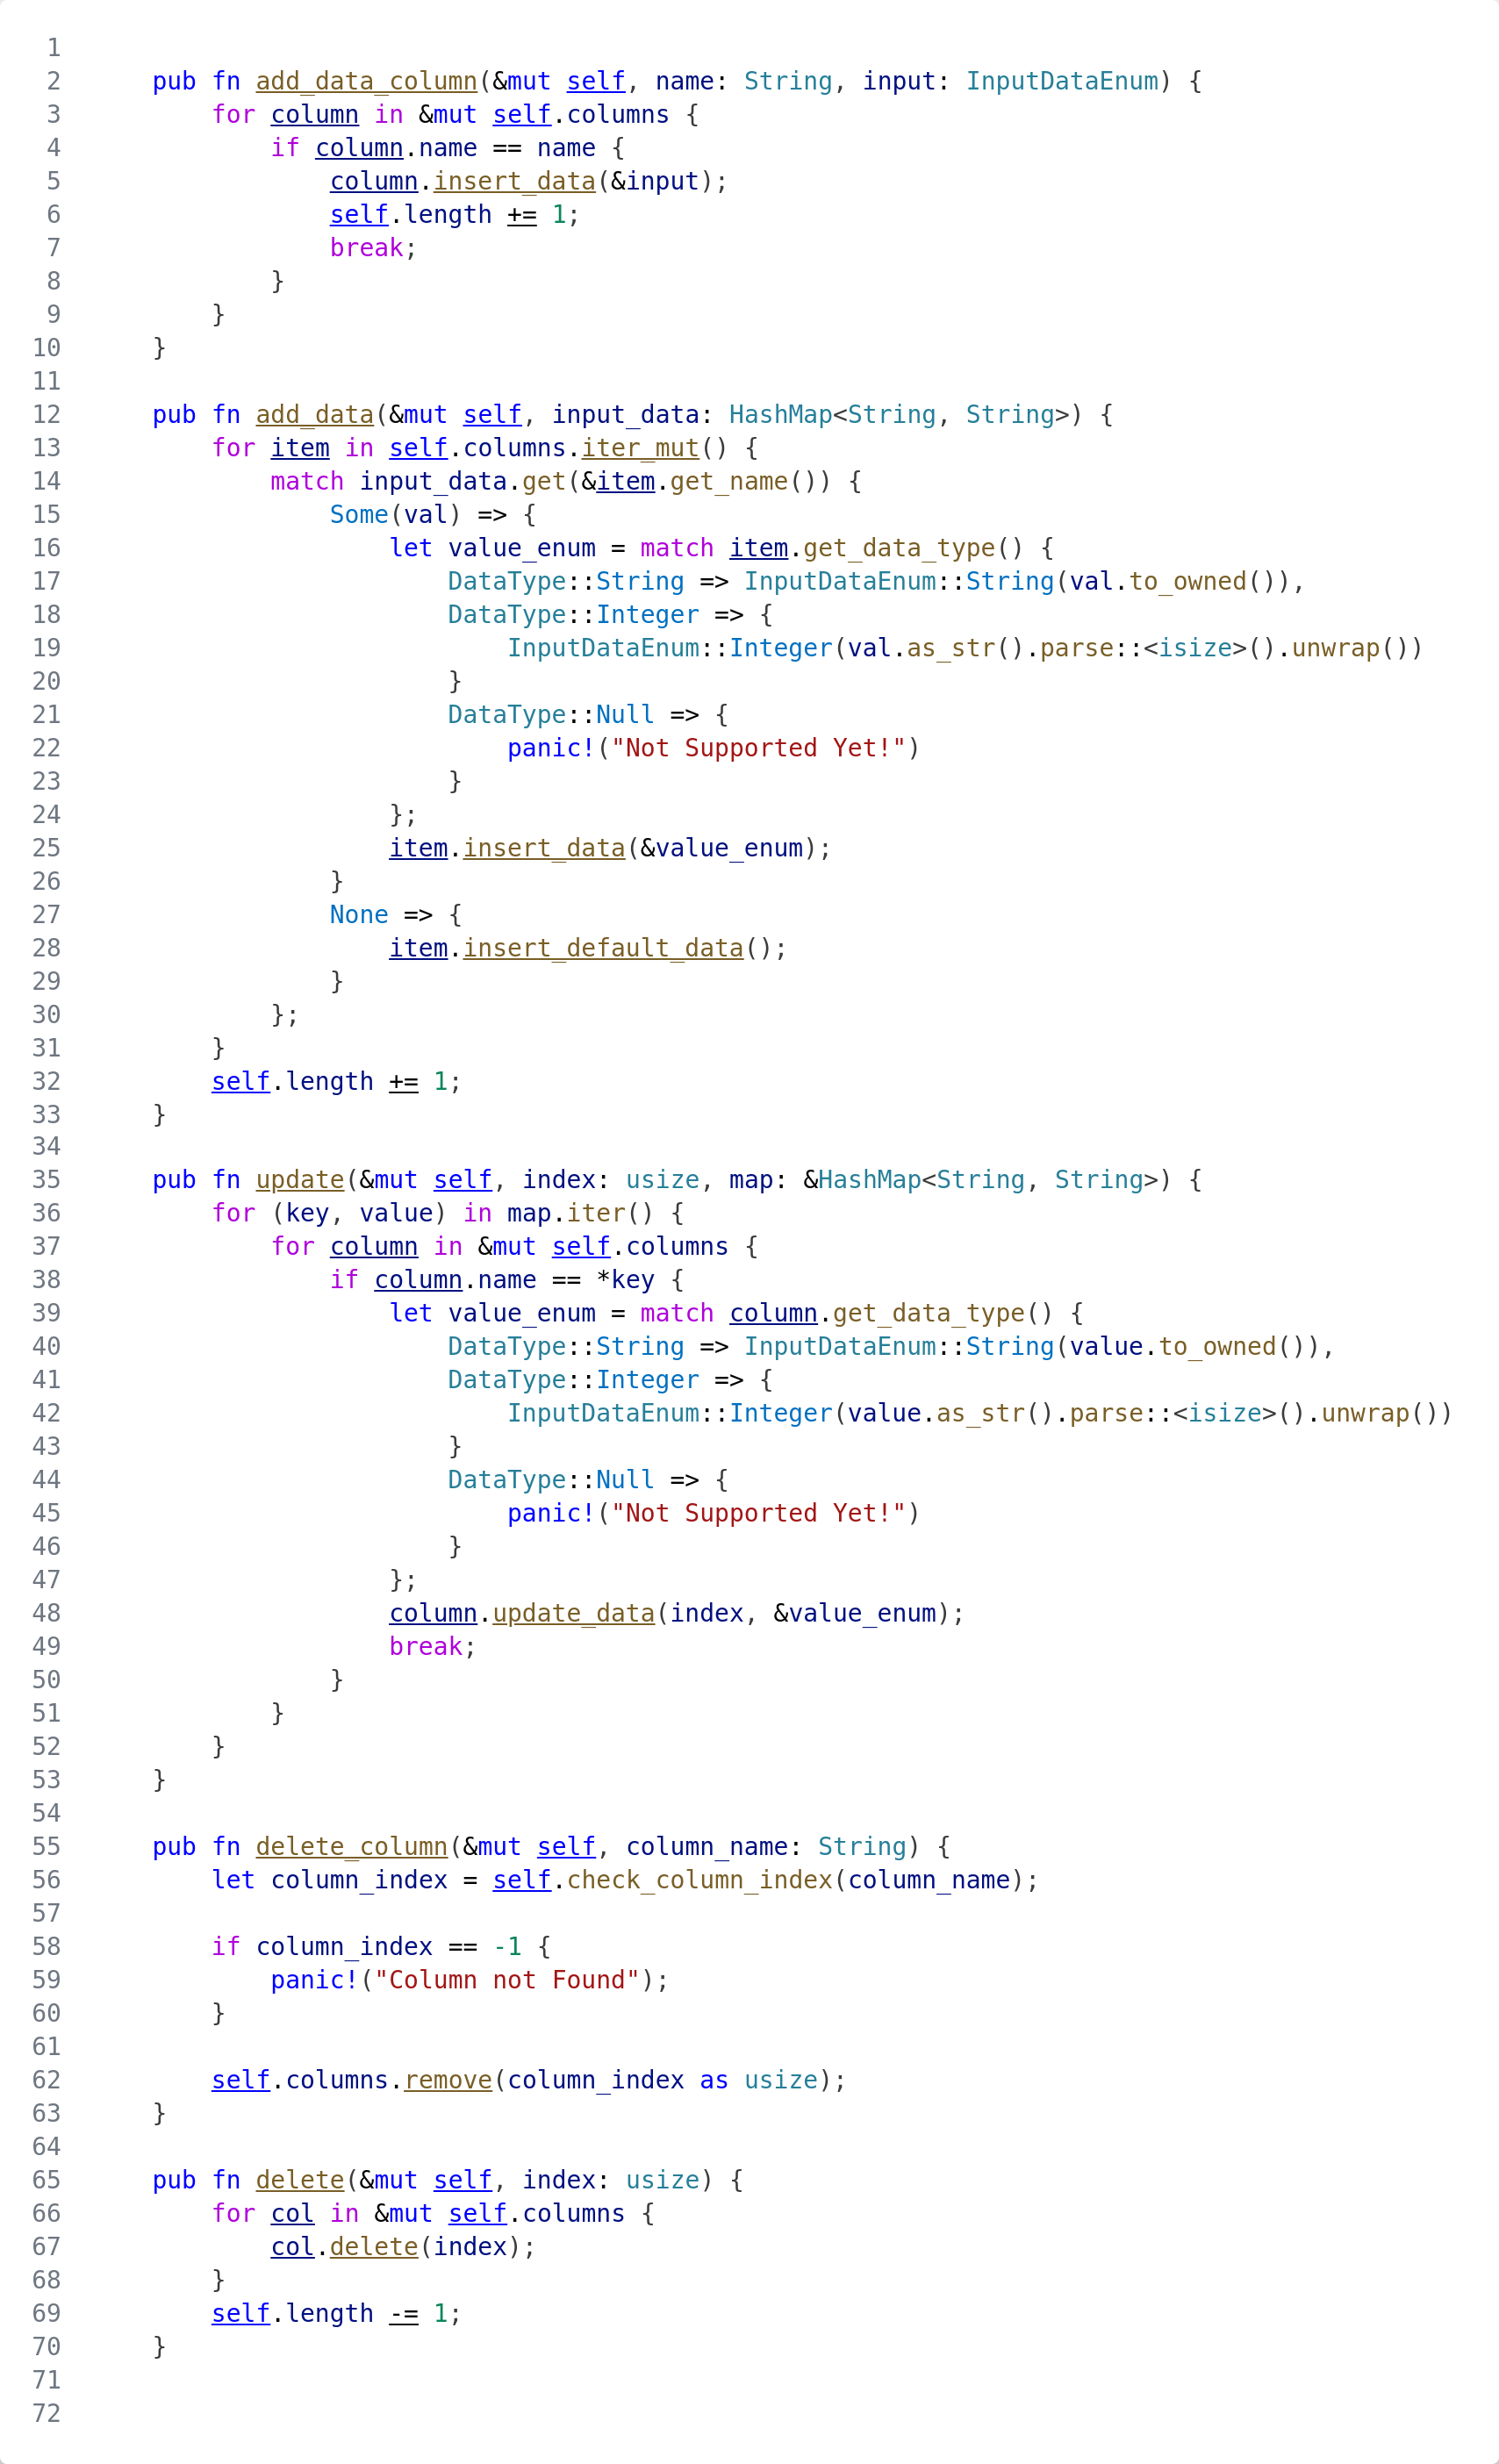
\includegraphics[width=0.7\textwidth]{gambar/lampiran/file-table-3.png}
  \caption{\emph{File} table.rs bagian 3}
\end{figure}

\begin{figure}[H]
  \centering{}
	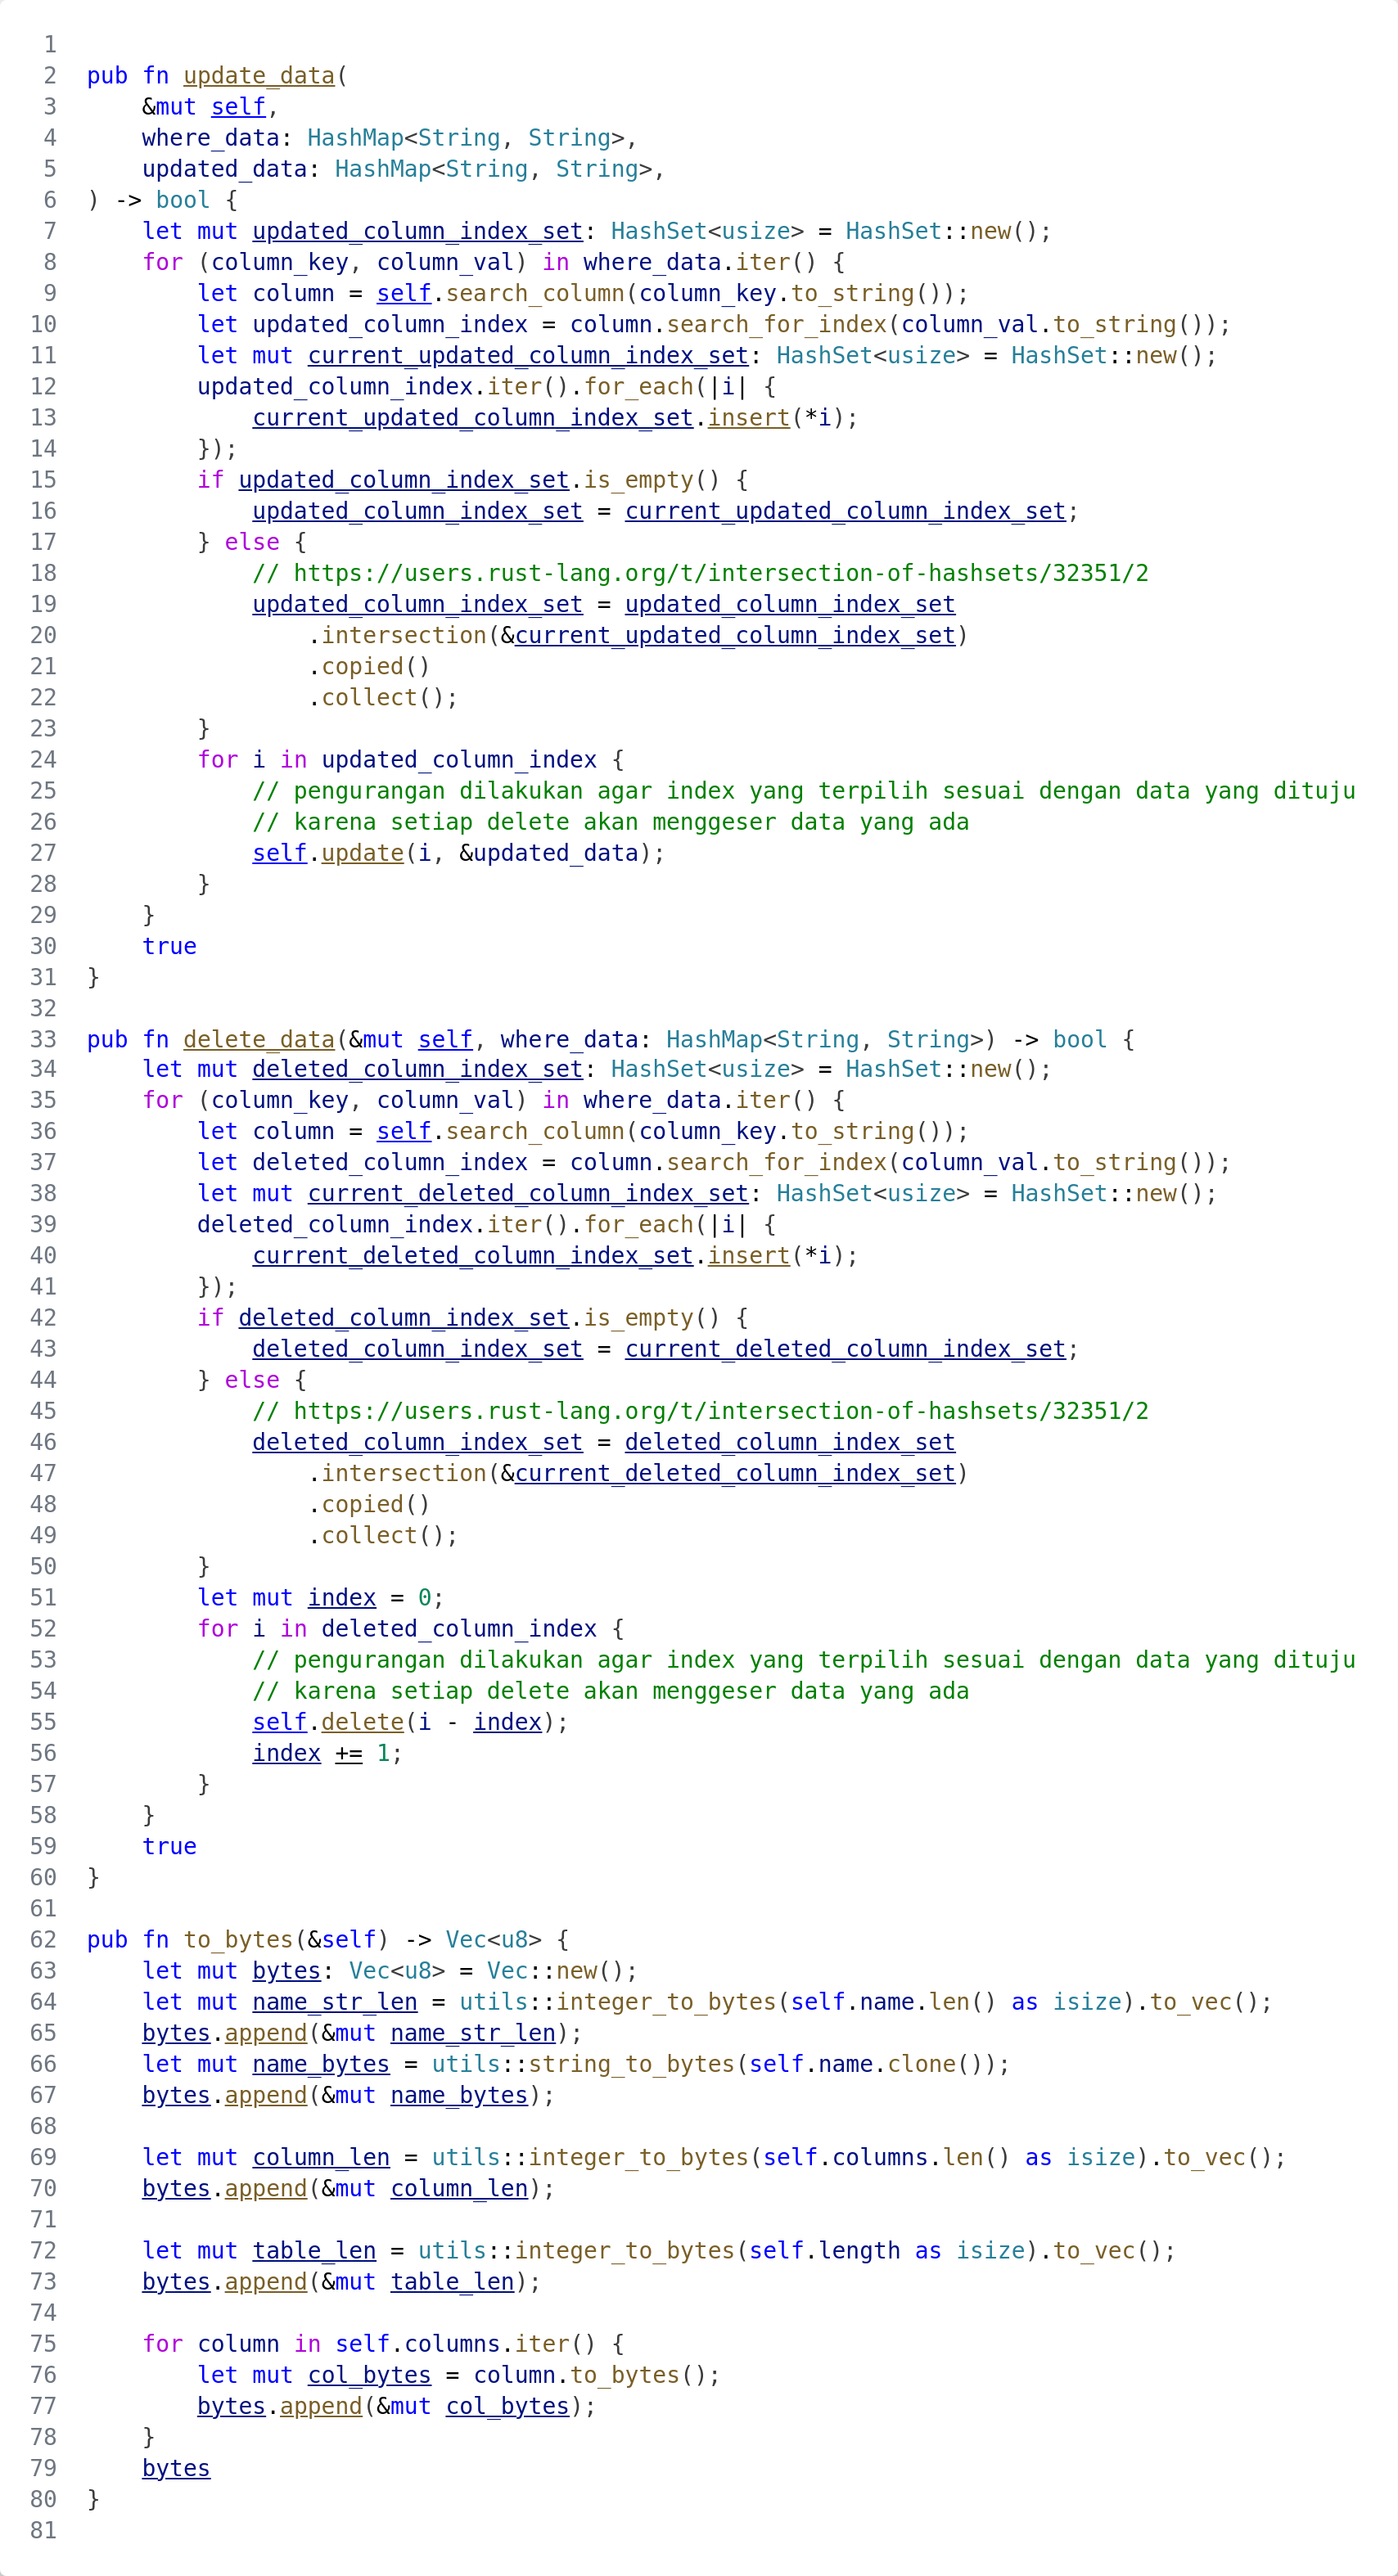
\includegraphics[width=0.7\textwidth]{gambar/lampiran/file-table-4.png}
  \caption{\emph{File} table.rs bagian 4}
\end{figure}

\begin{figure}[H]
  \centering{}
	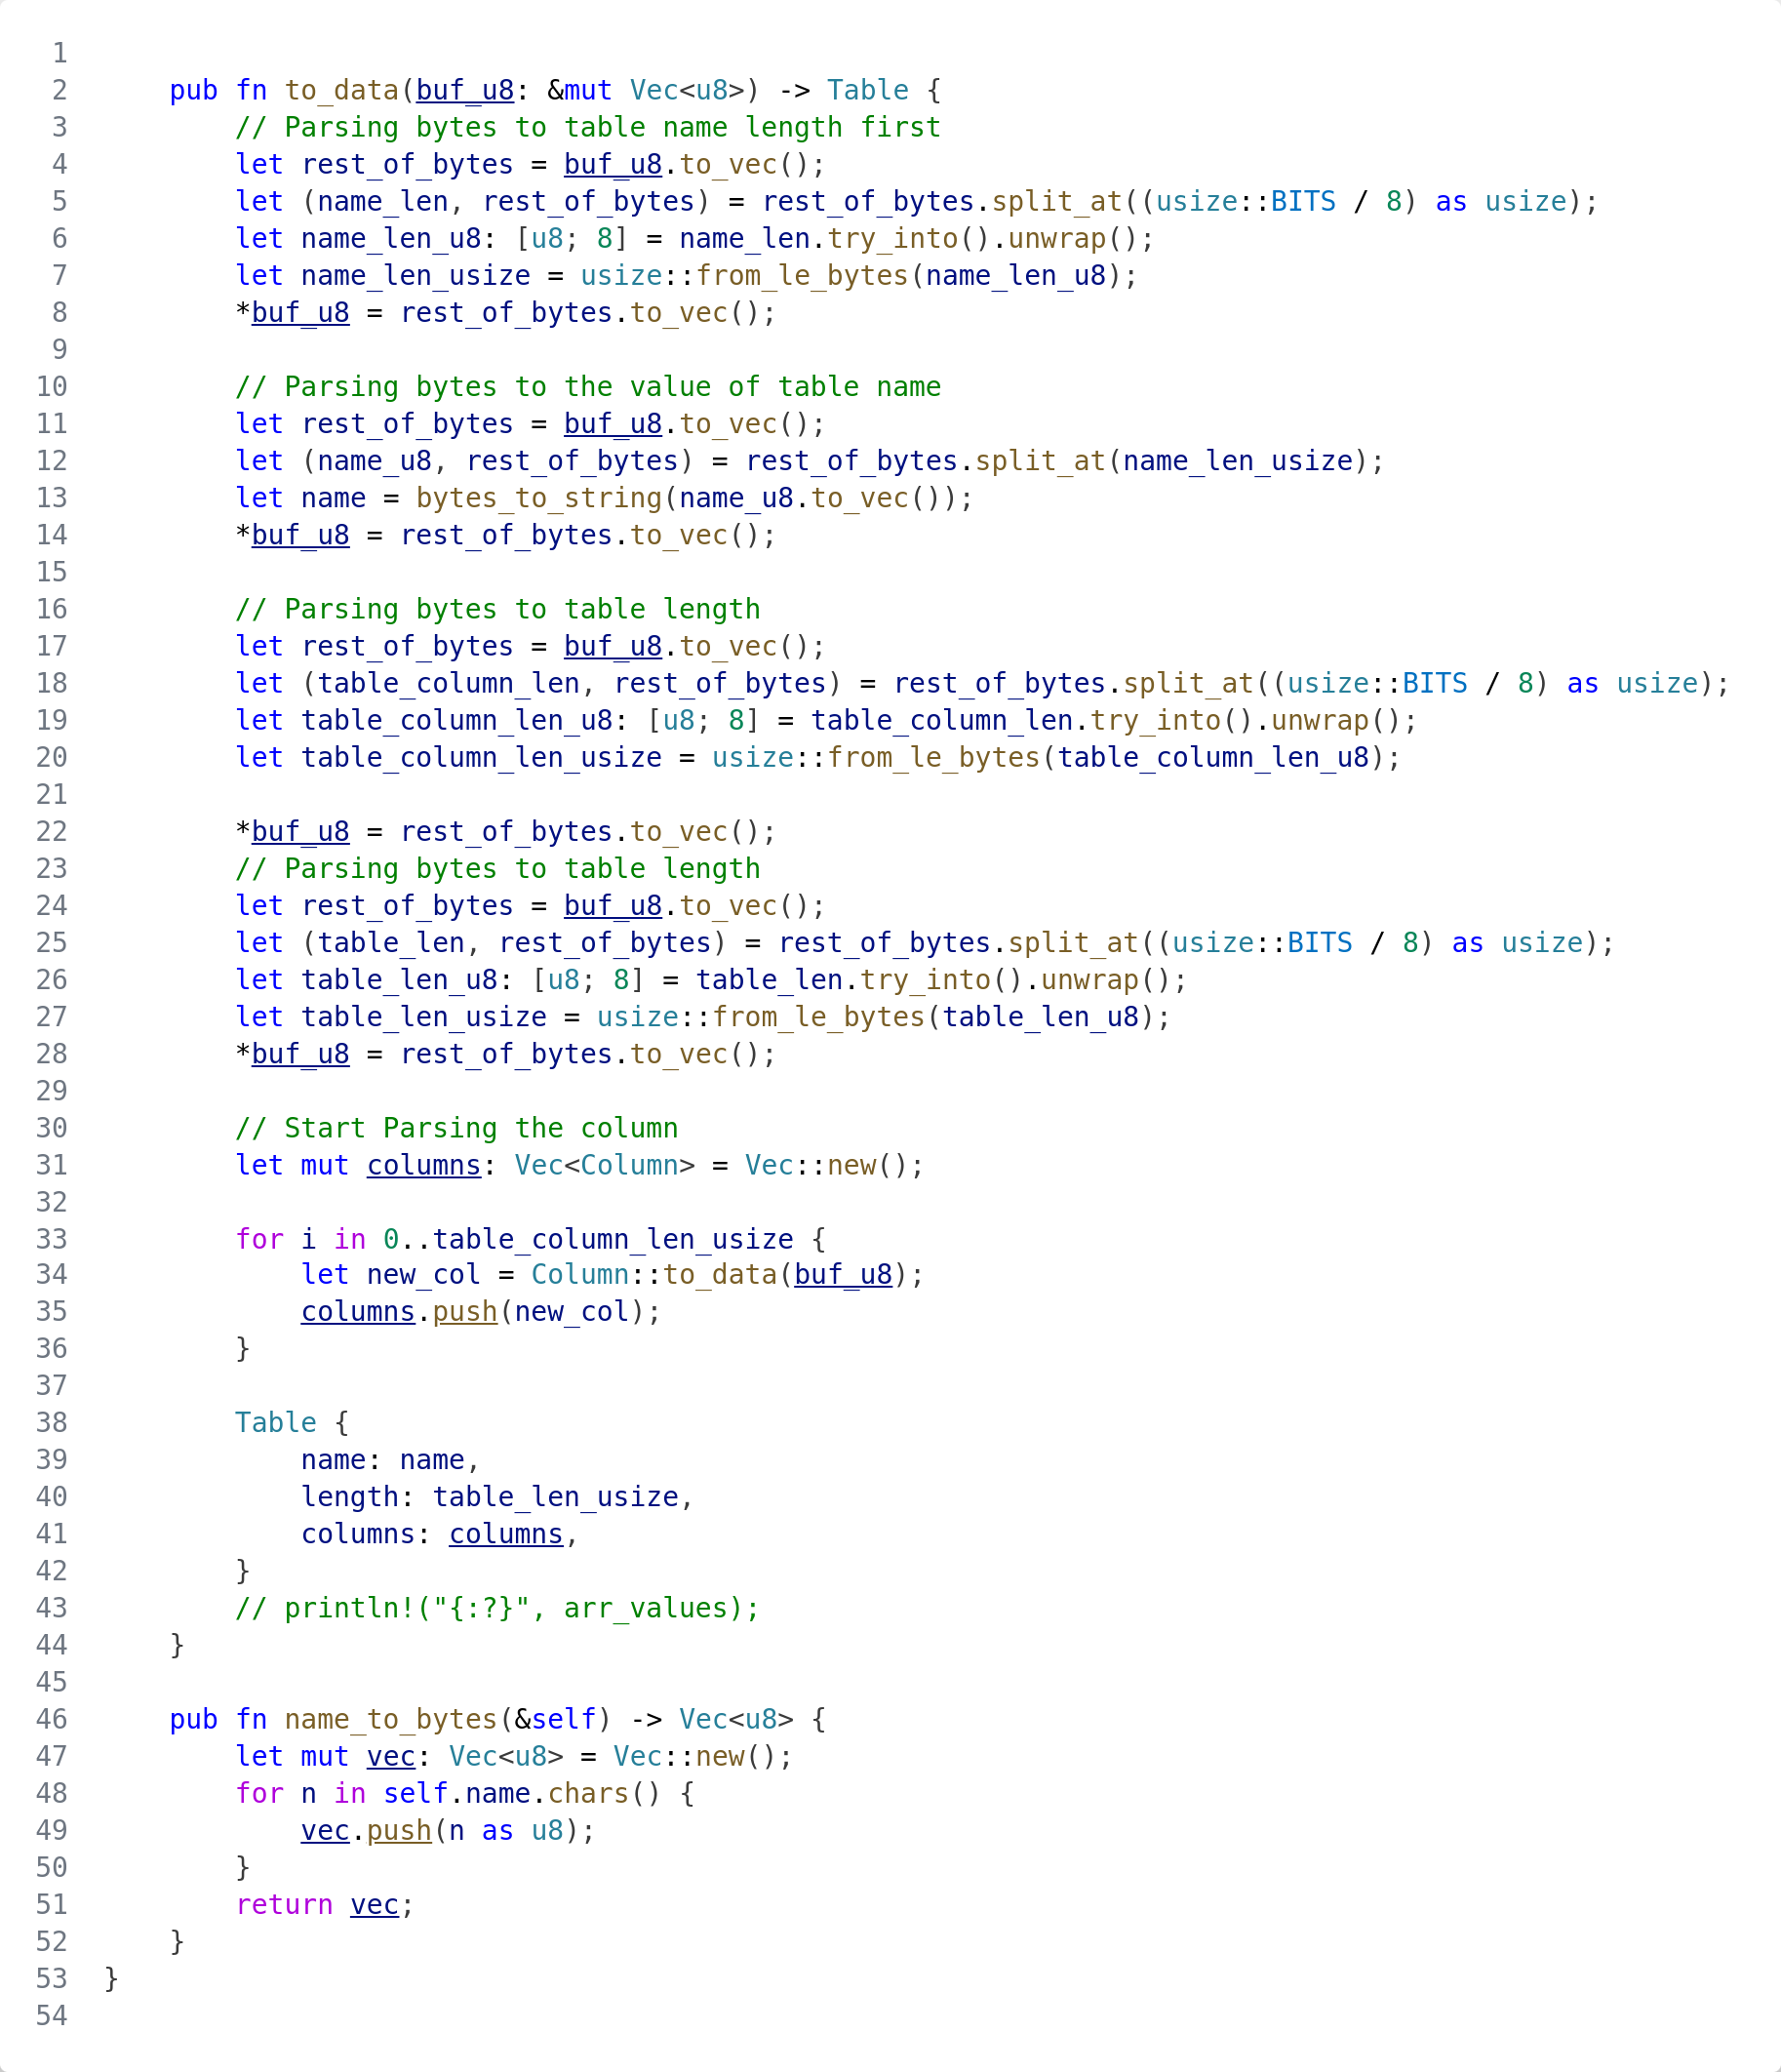
\includegraphics[width=0.7\textwidth]{gambar/lampiran/file-table-5.png}
  \caption{\emph{File} table.rs bagian 5}
\end{figure}

\begin{figure}[H]
  \centering{}
	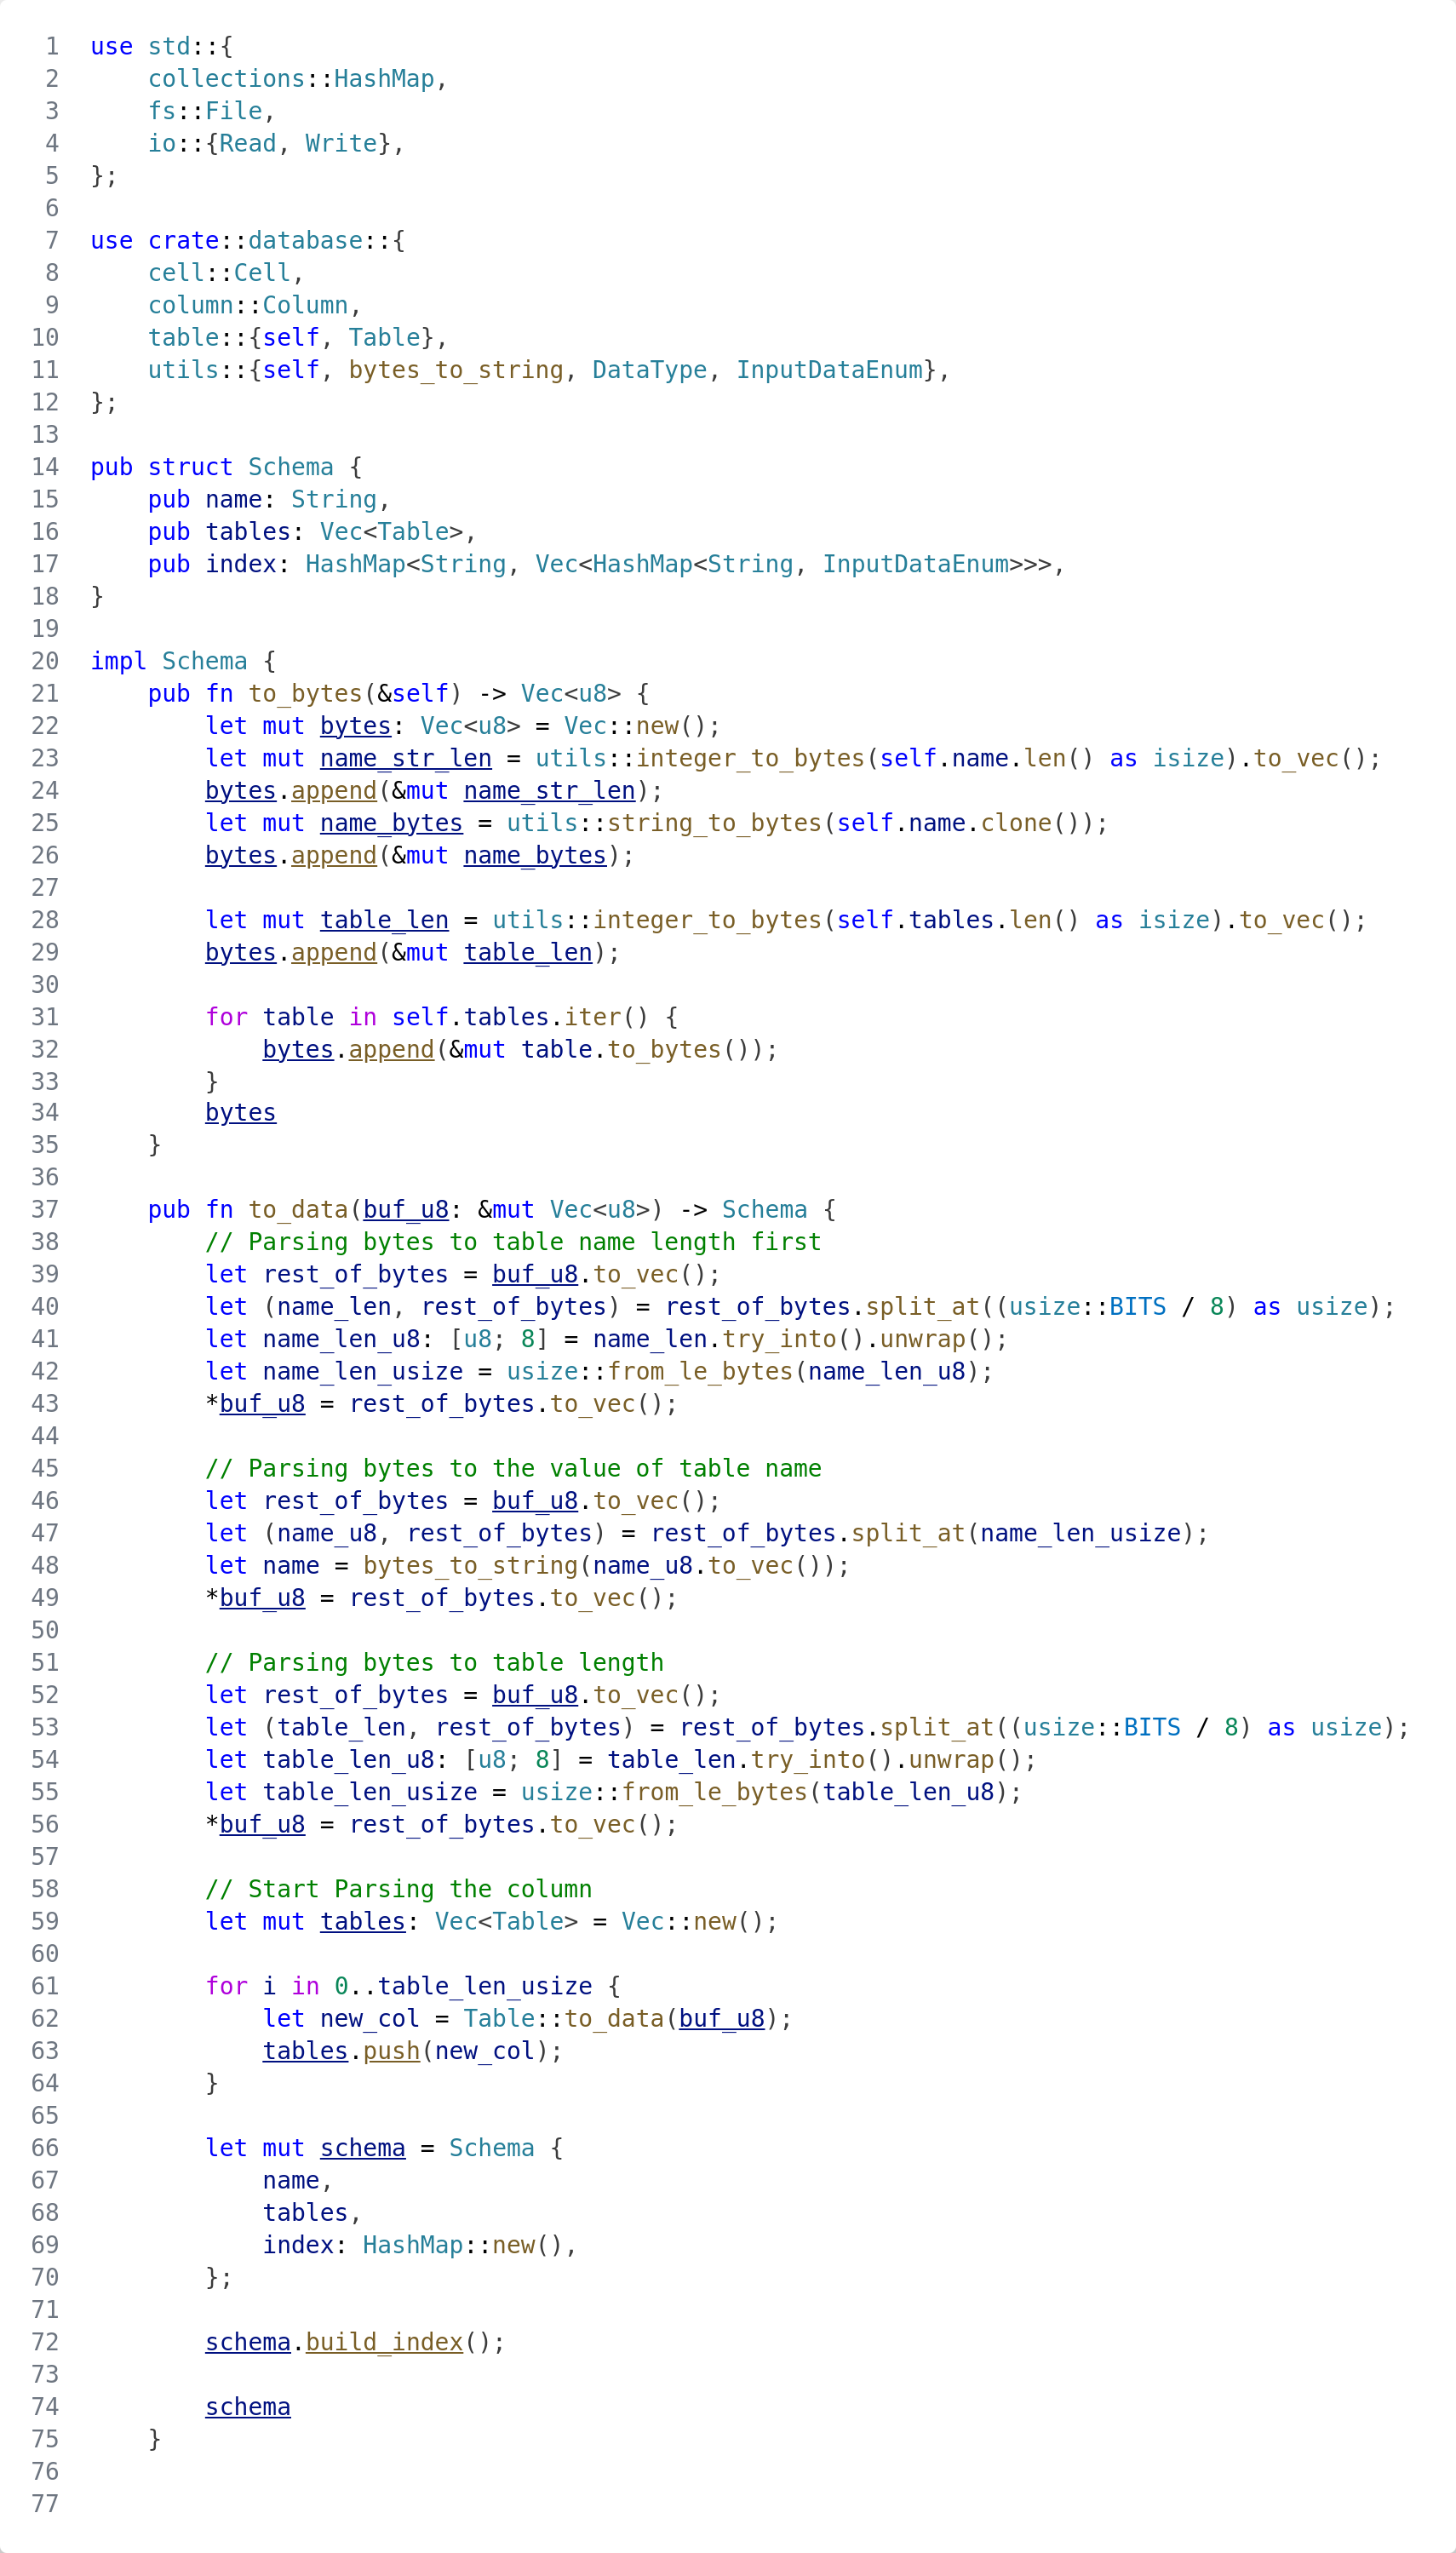
\includegraphics[width=0.6\textwidth]{gambar/lampiran/file-schema-1.png}
  \caption{\emph{File} schema.rs bagian 1}
\end{figure}

\begin{figure}[H]
  \centering{}
	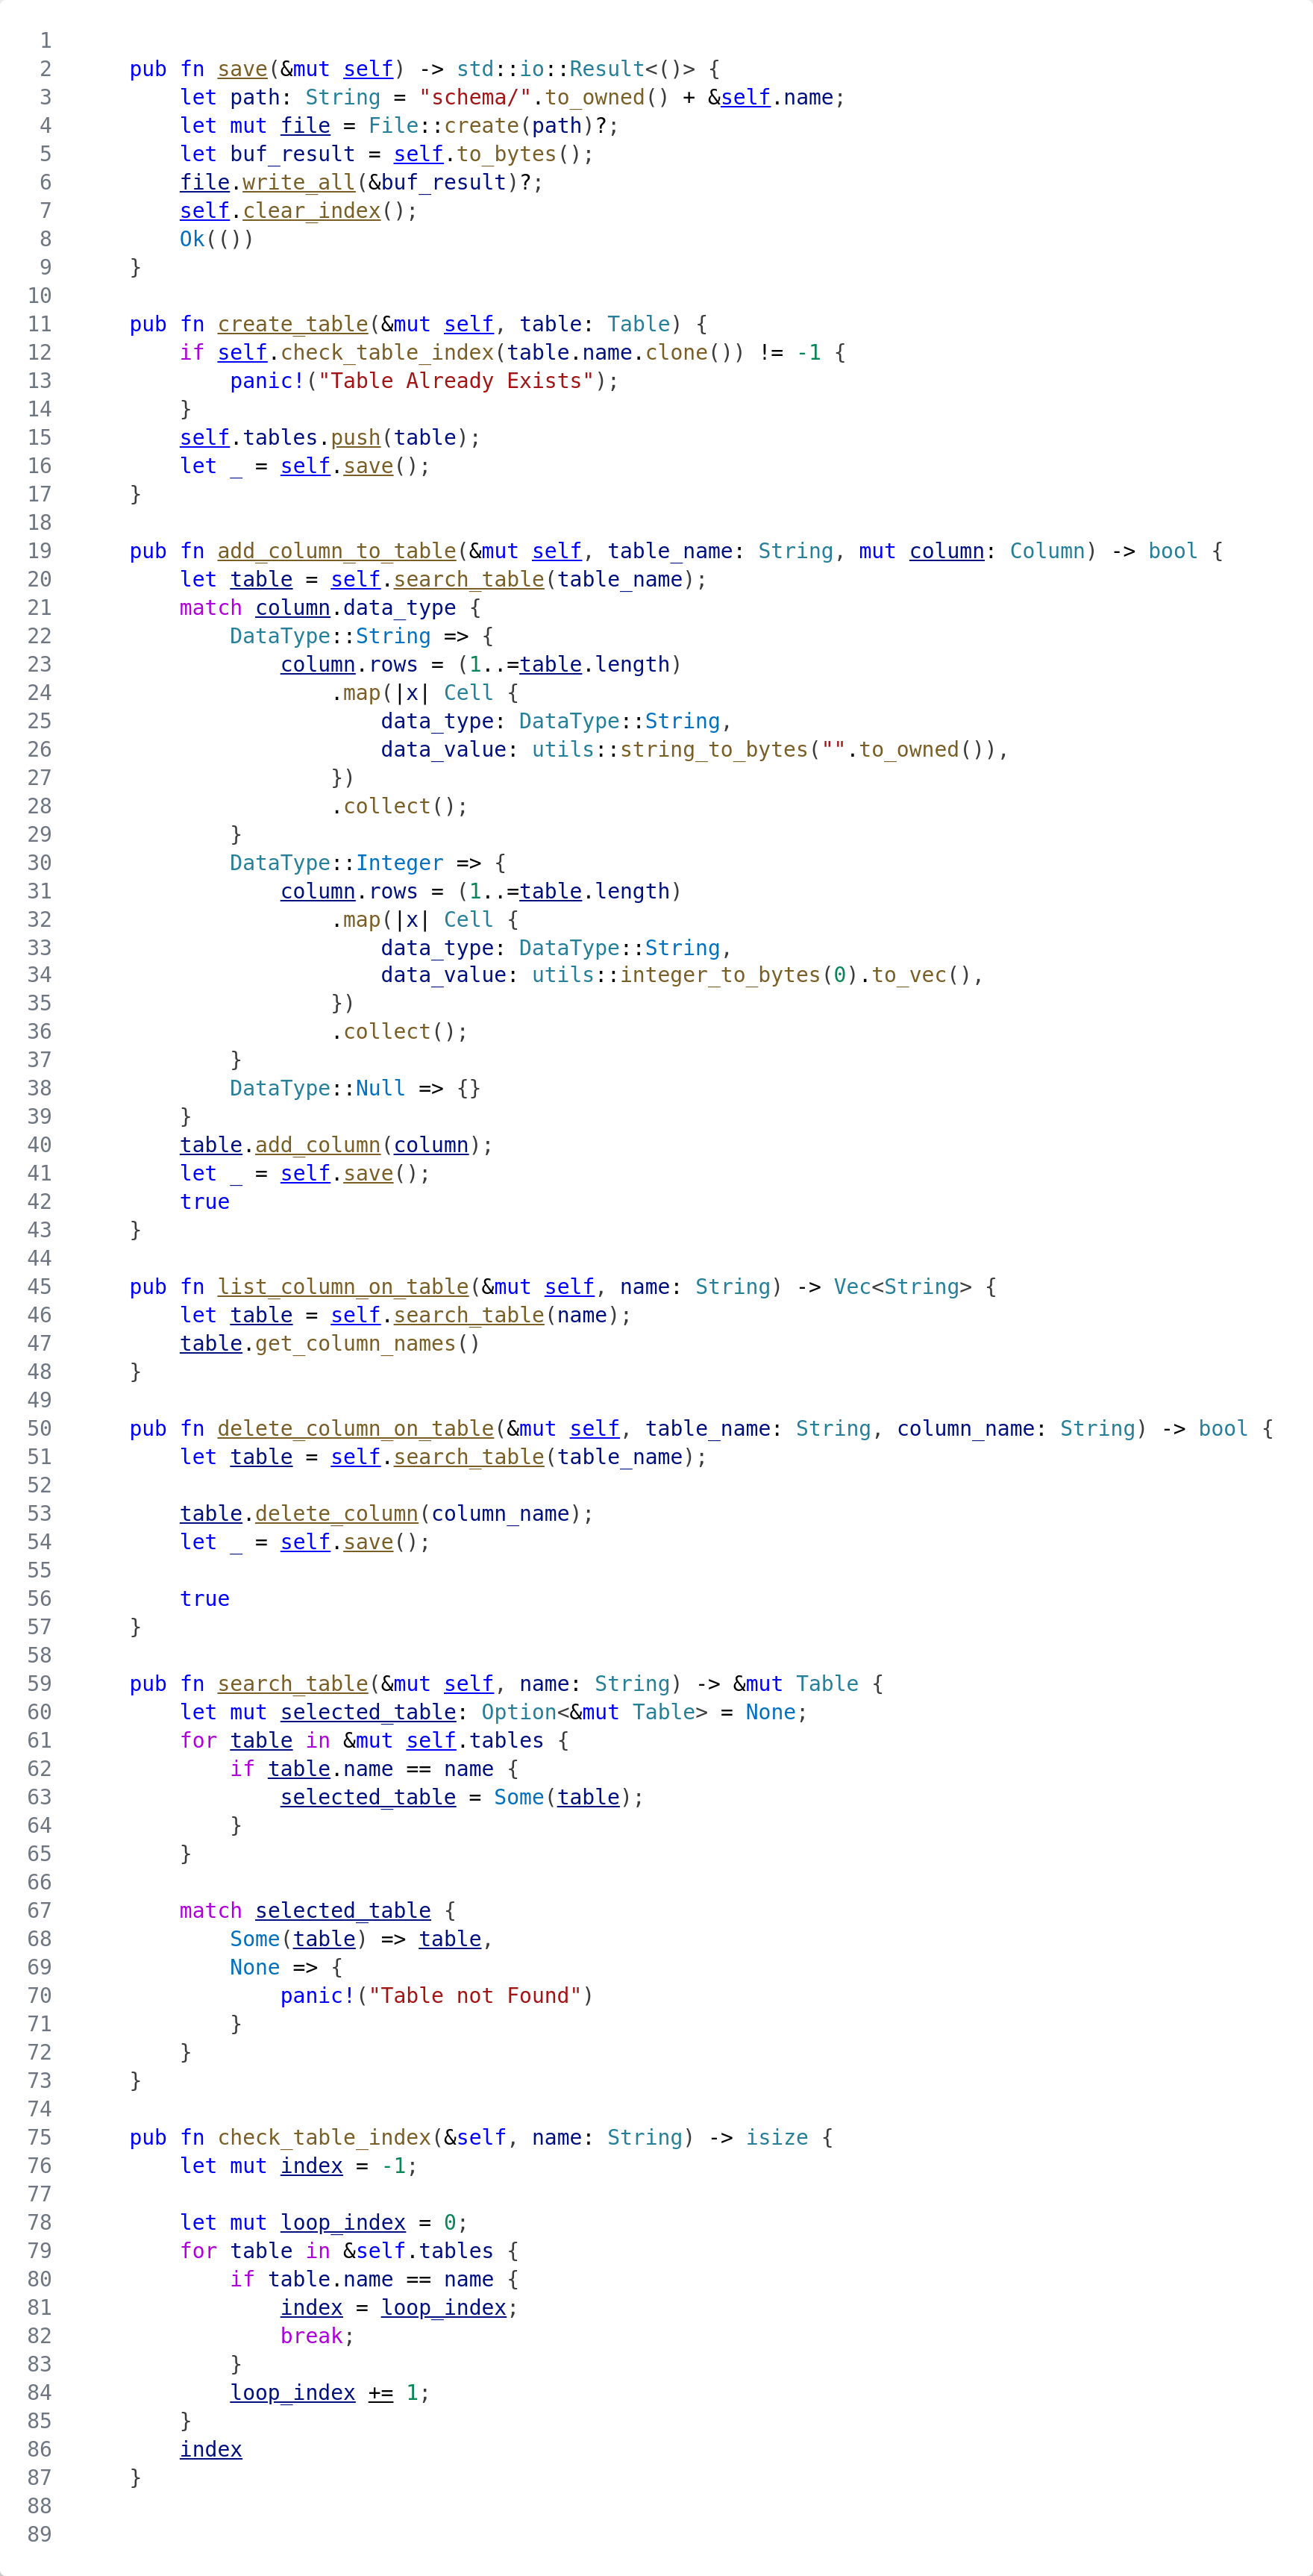
\includegraphics[width=0.6\textwidth]{gambar/lampiran/file-schema-2.png}
  \caption{\emph{File} schema.rs bagian 2}
\end{figure}

\begin{figure}[H]
  \centering{}
	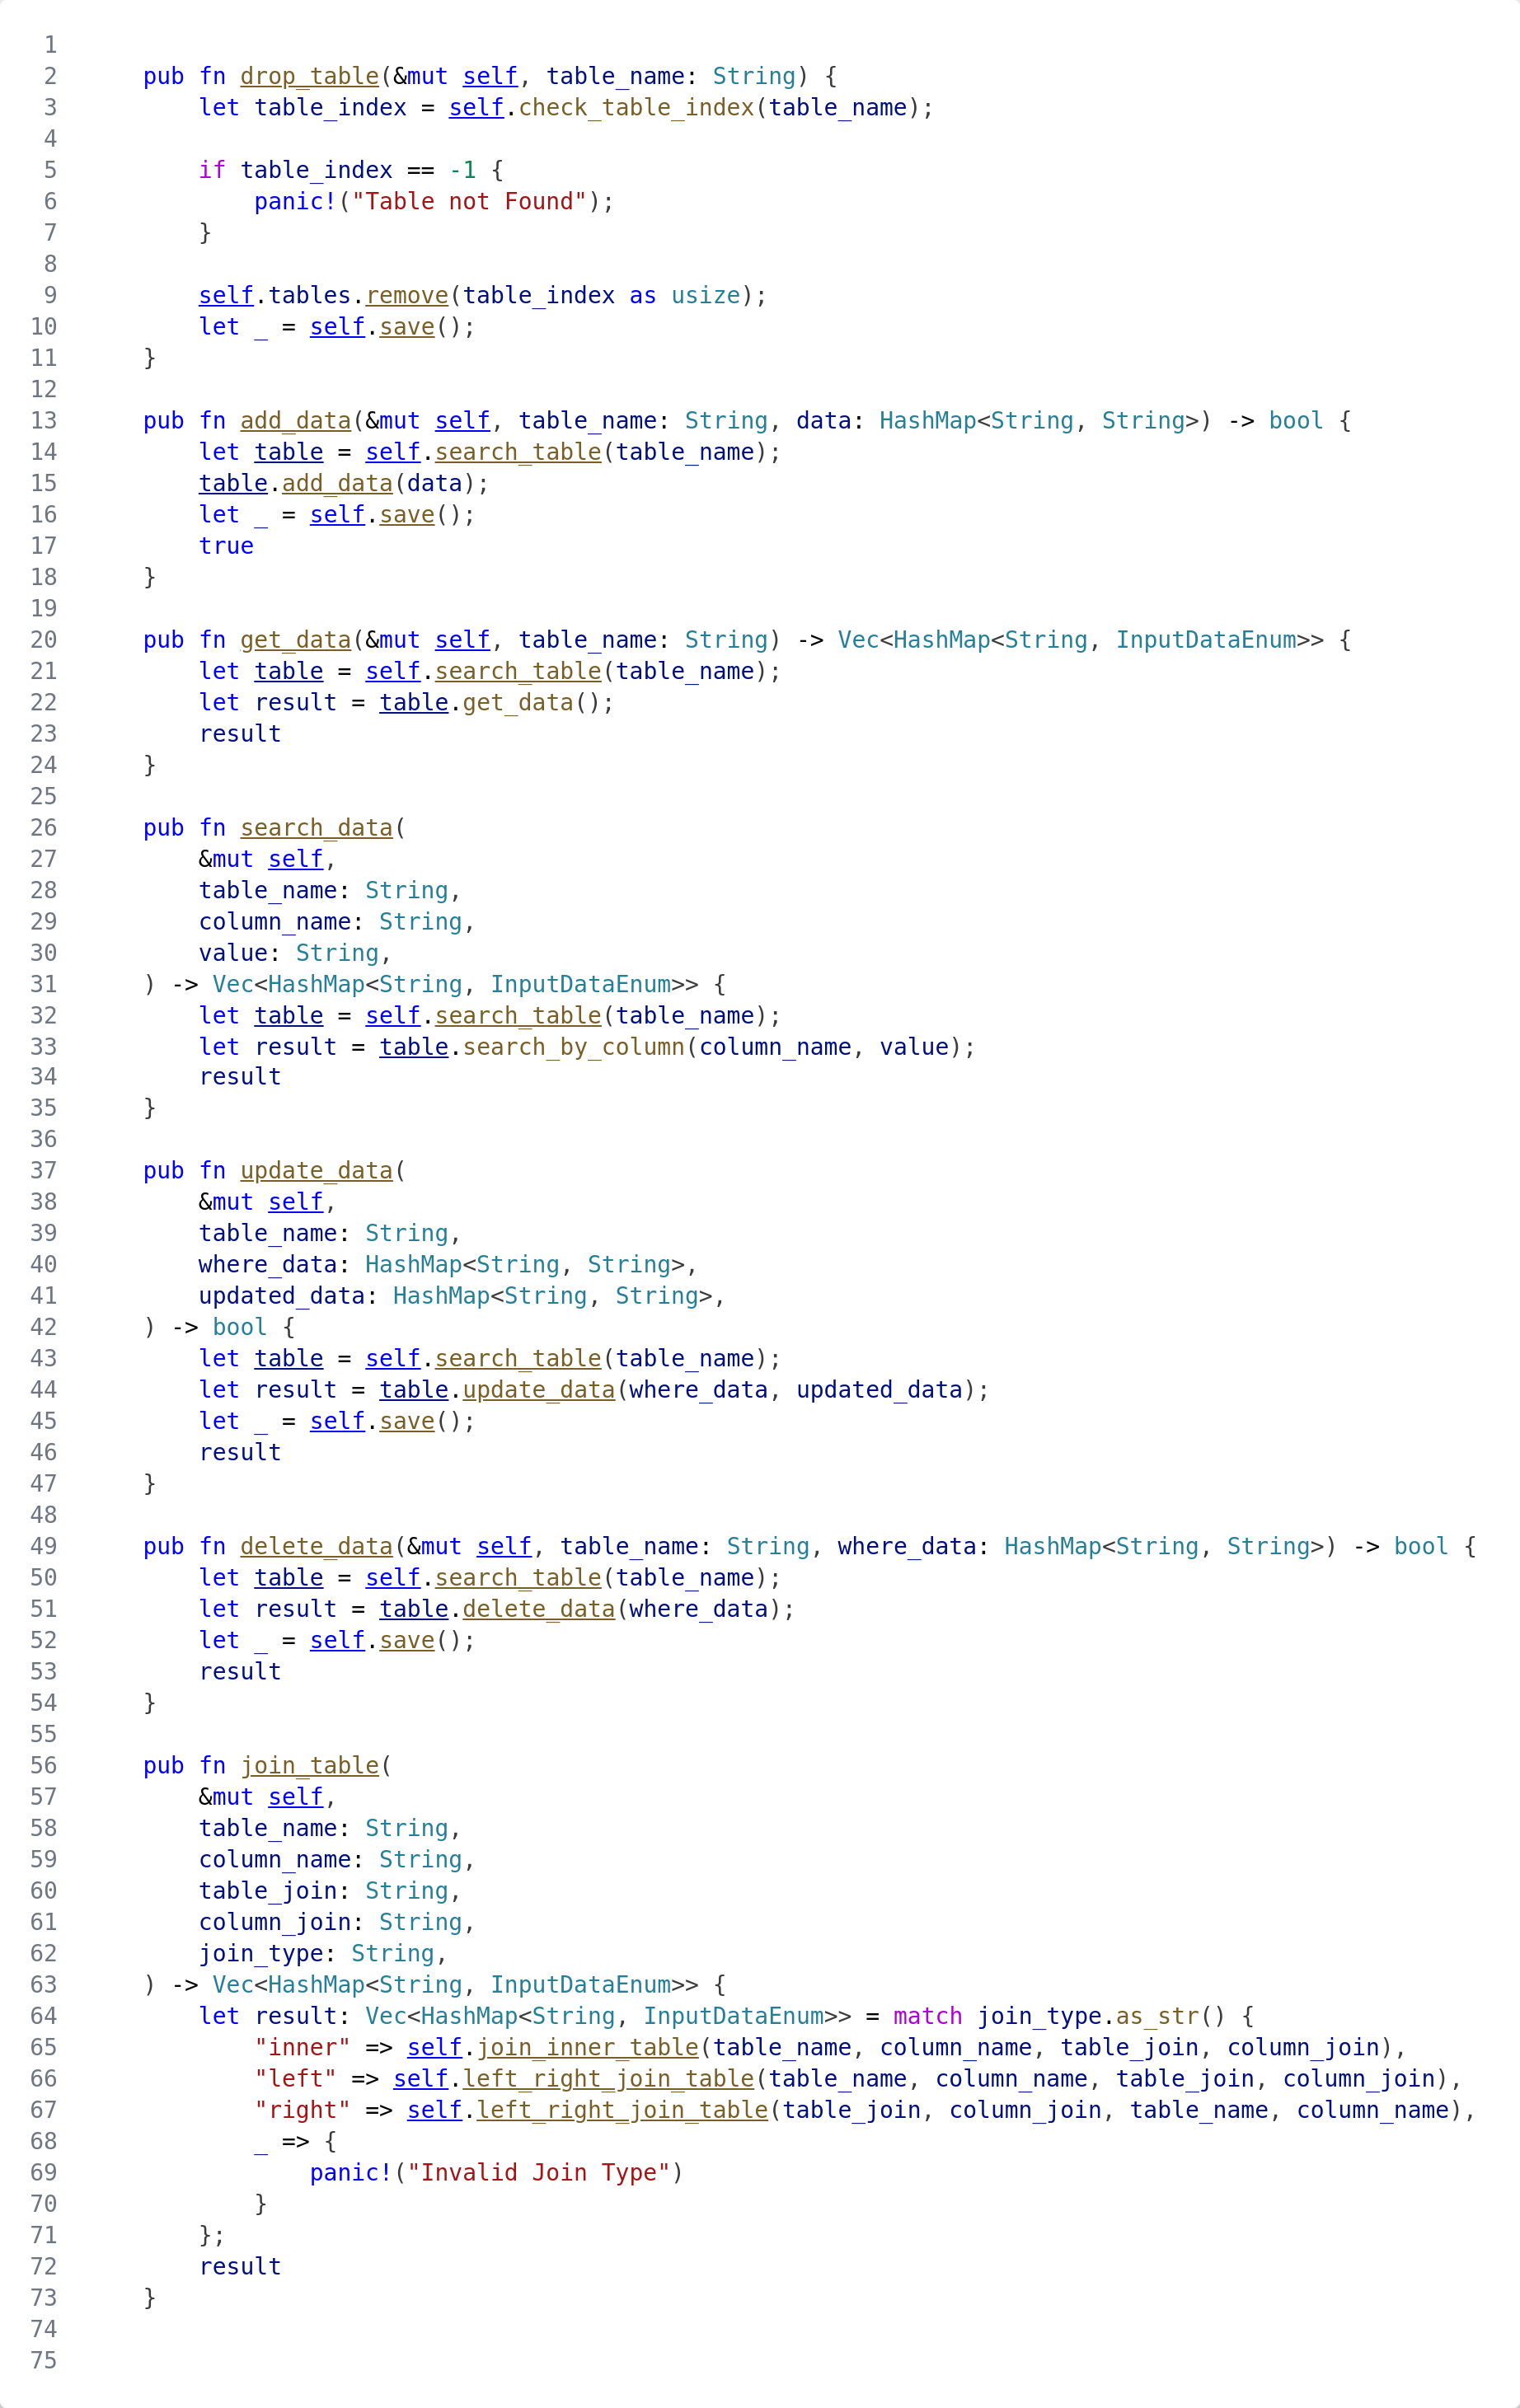
\includegraphics[width=0.6\textwidth]{gambar/lampiran/file-schema-3.png}
  \caption{\emph{File} schema.rs bagian 3}
\end{figure}

\begin{figure}[H]
  \centering{}
	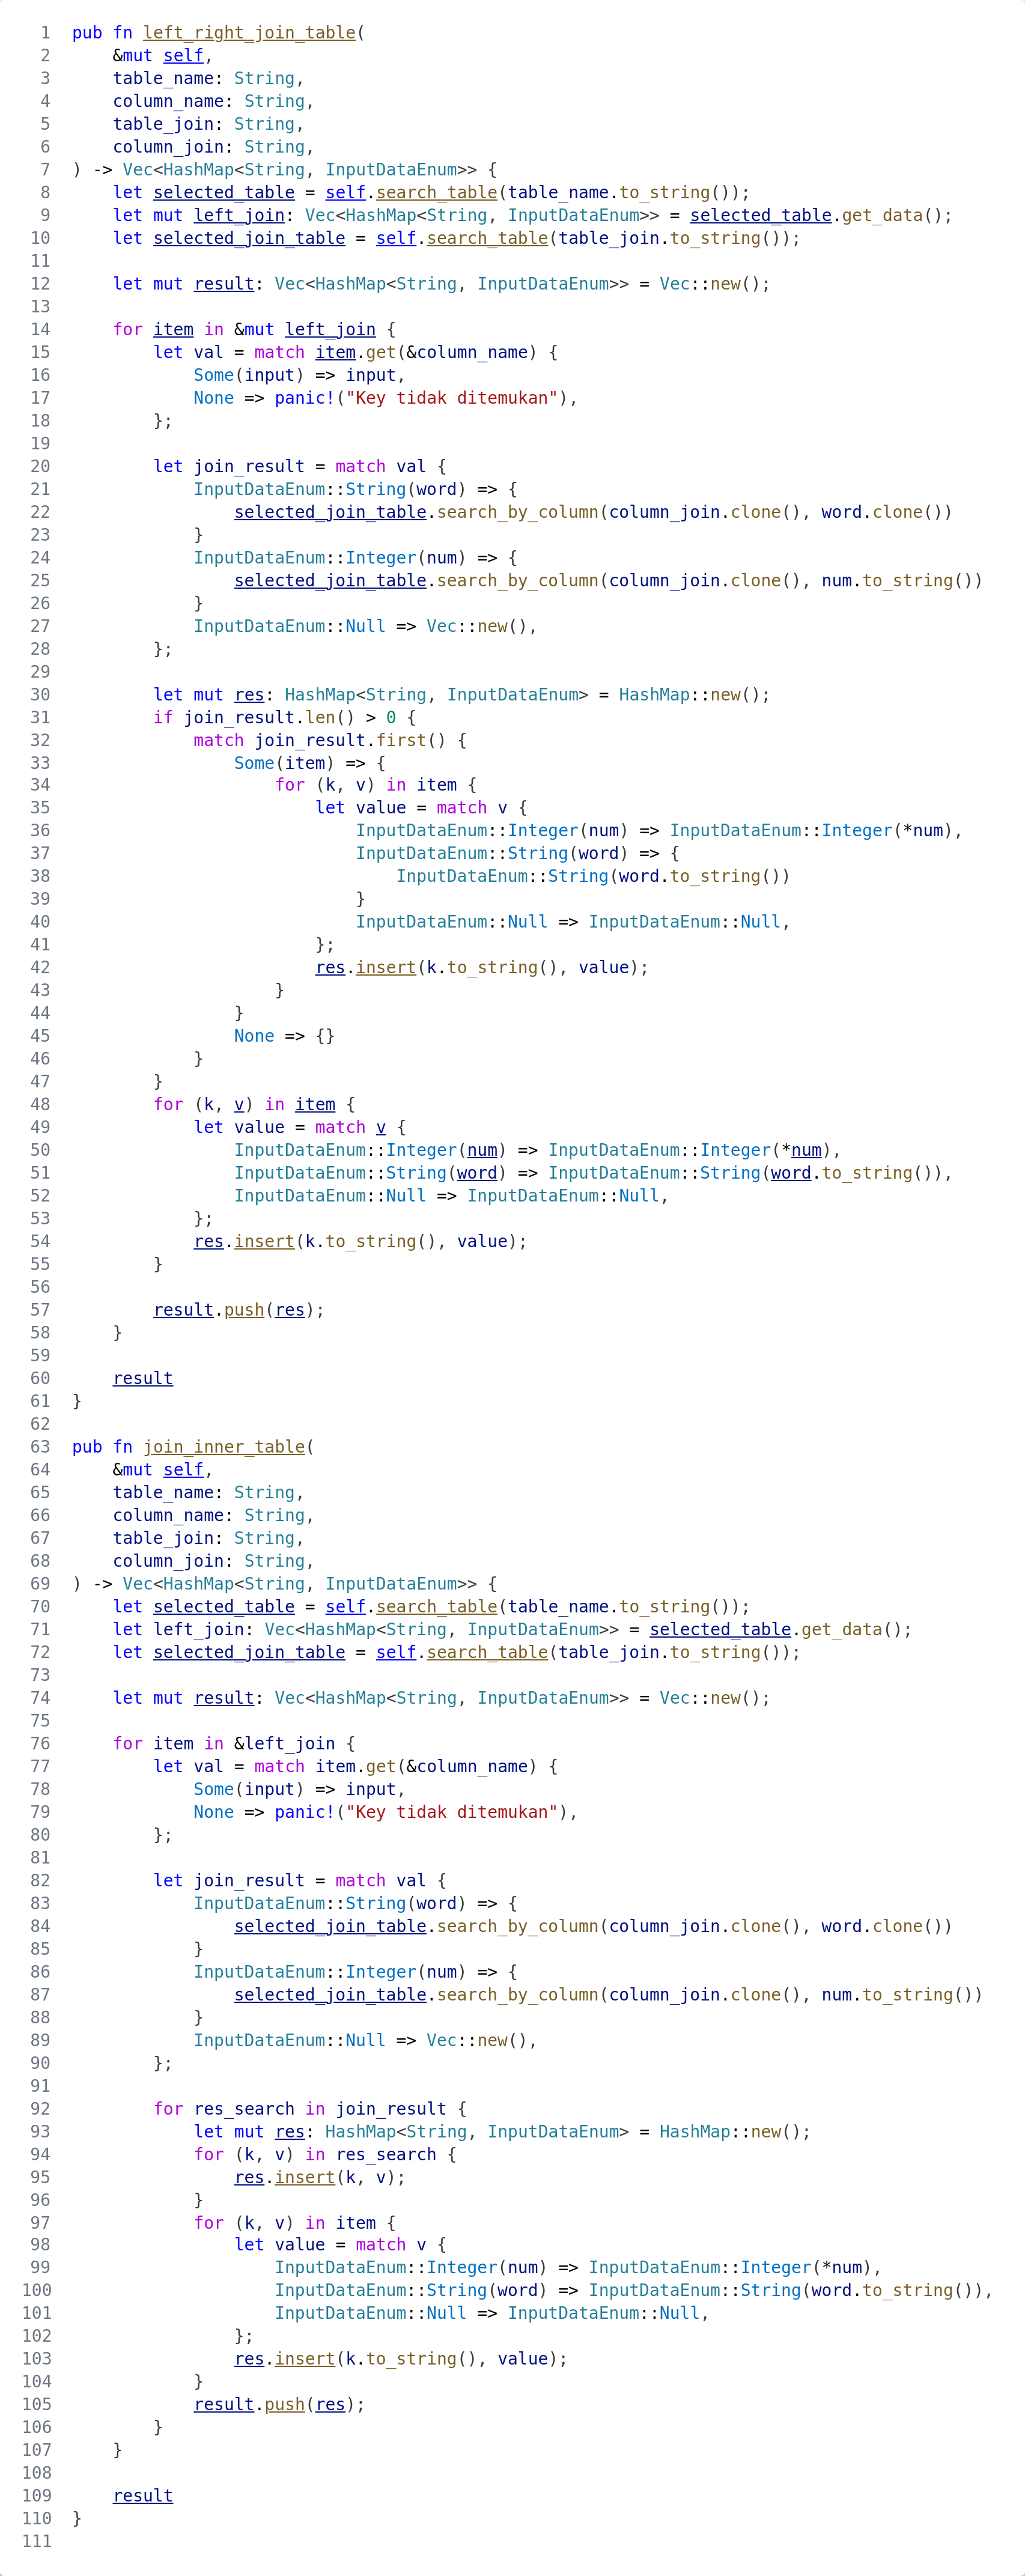
\includegraphics[width=0.4\textwidth]{gambar/lampiran/file-schema-4.png}
  \caption{\emph{File} schema.rs bagian 4}
\end{figure}

\begin{figure}[H]
  \centering{}
	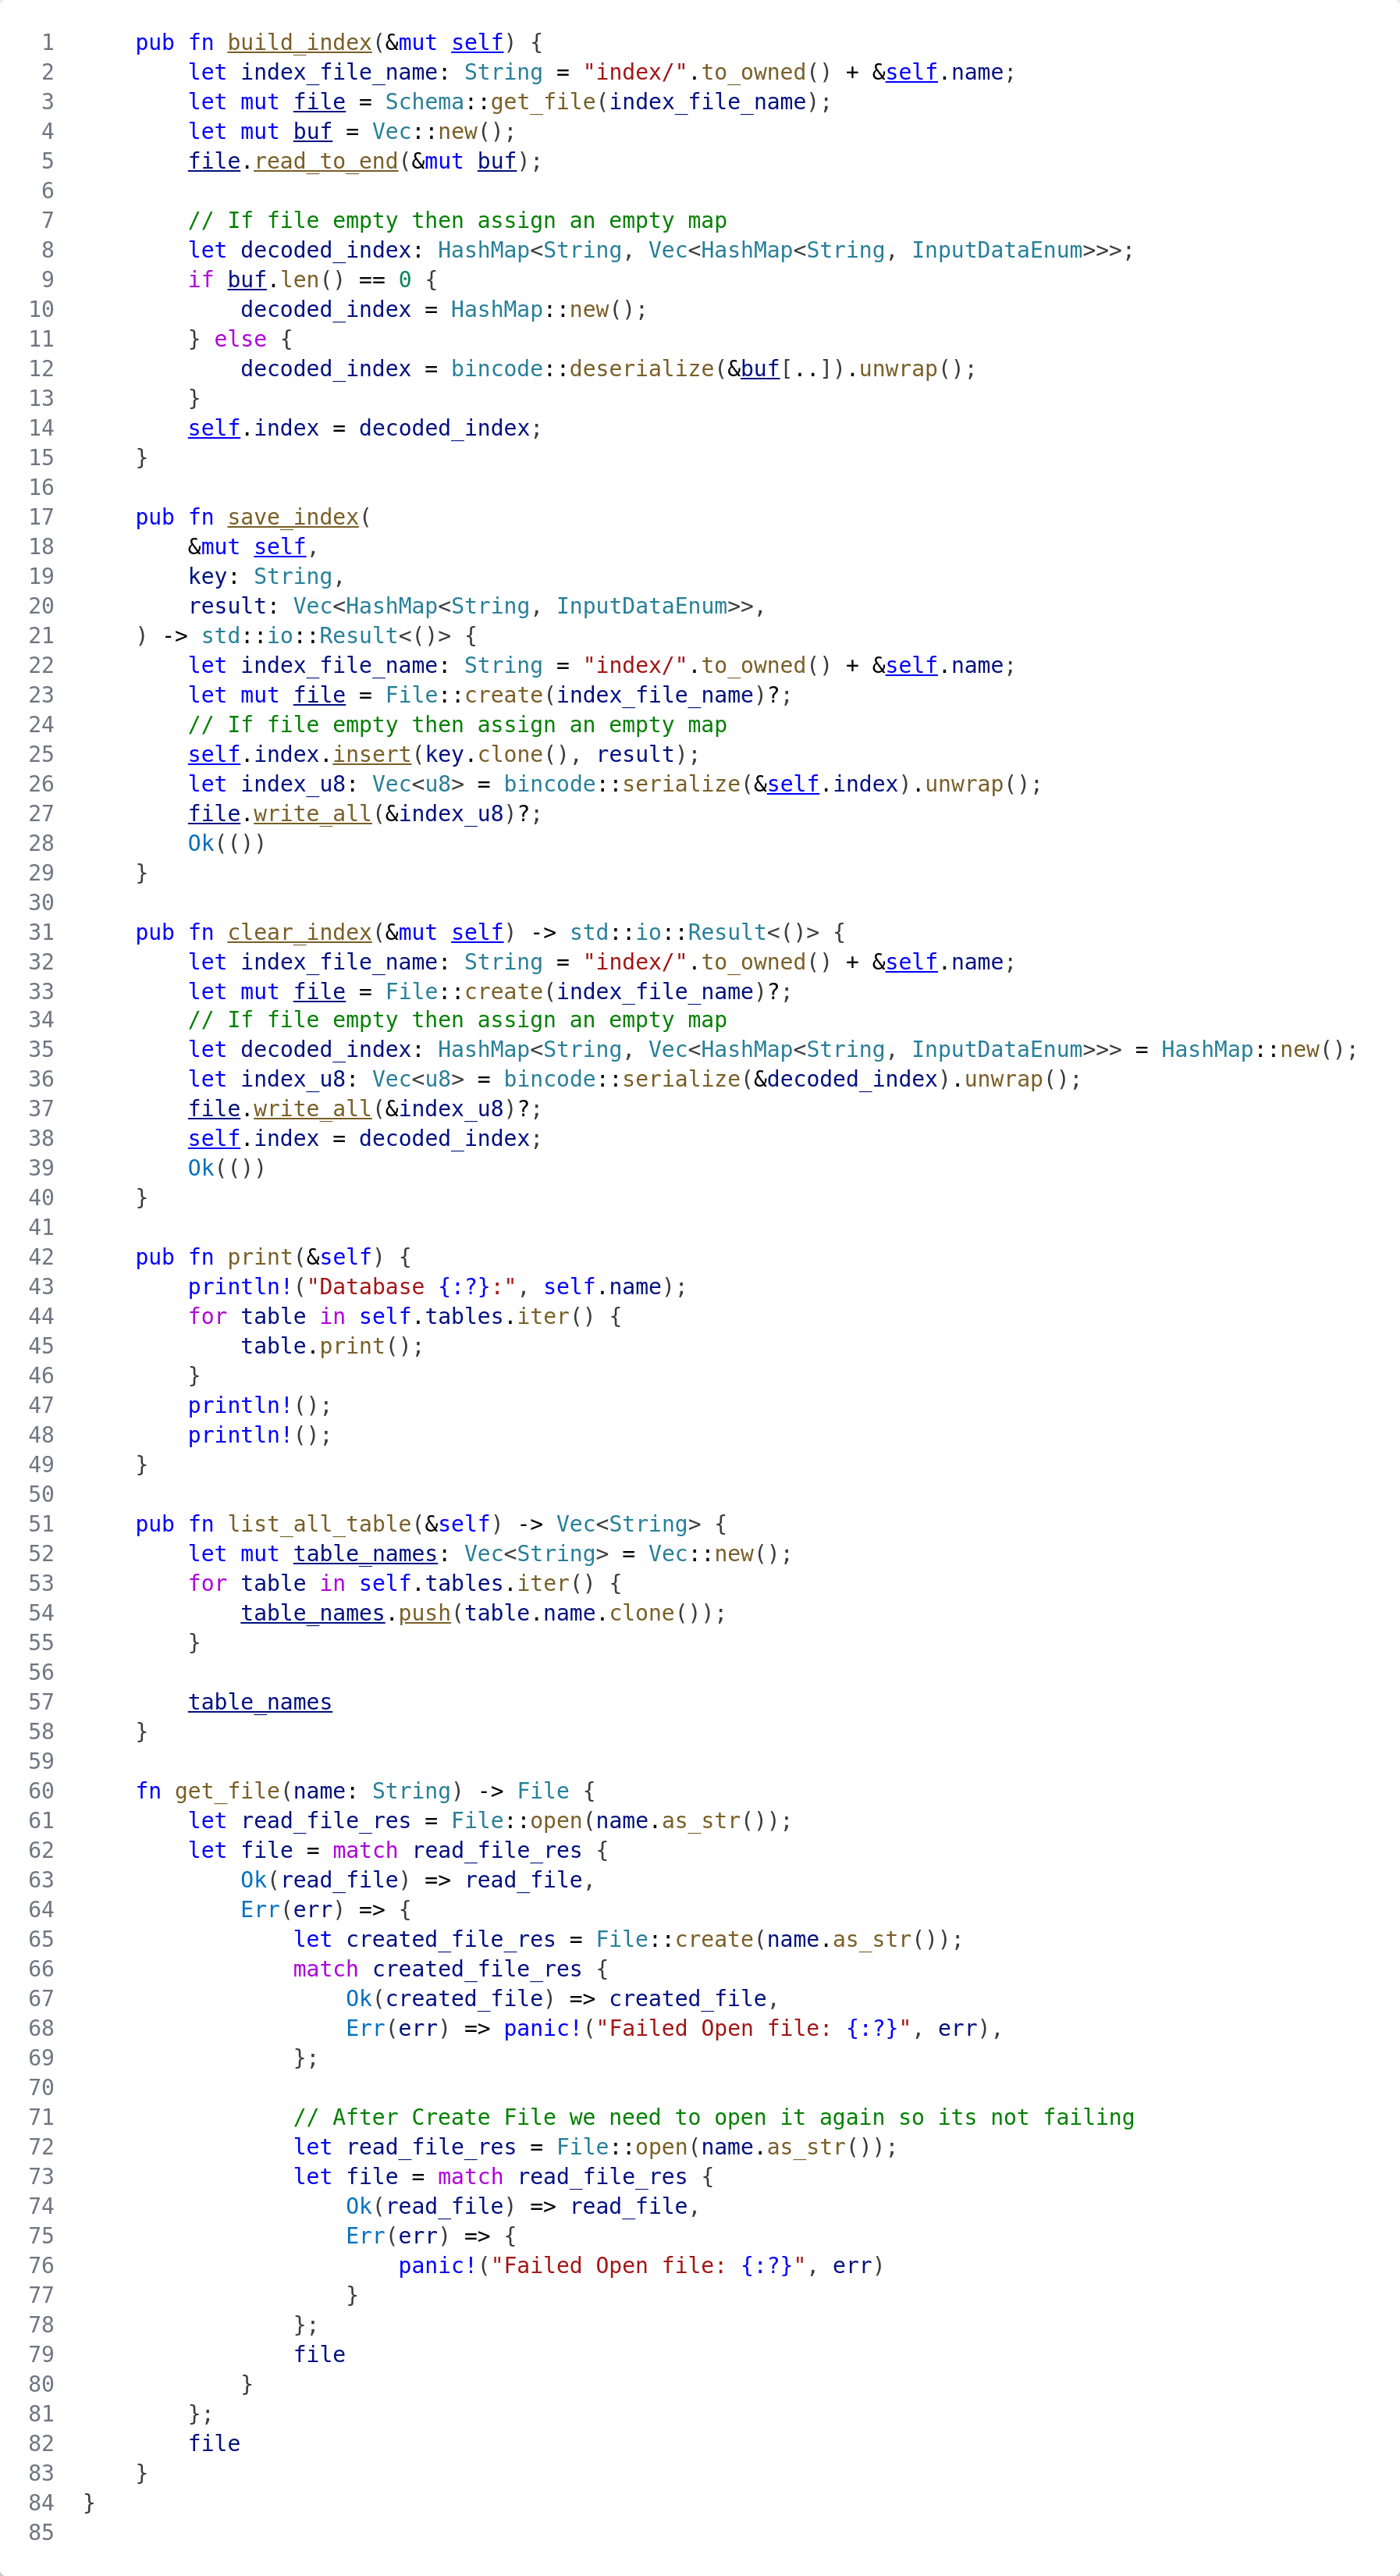
\includegraphics[width=0.6\textwidth]{gambar/lampiran/file-schema-5.png}
  \caption{\emph{File} schema.rs bagian 5}
\end{figure}

\begin{figure}[H]
  \centering{}
	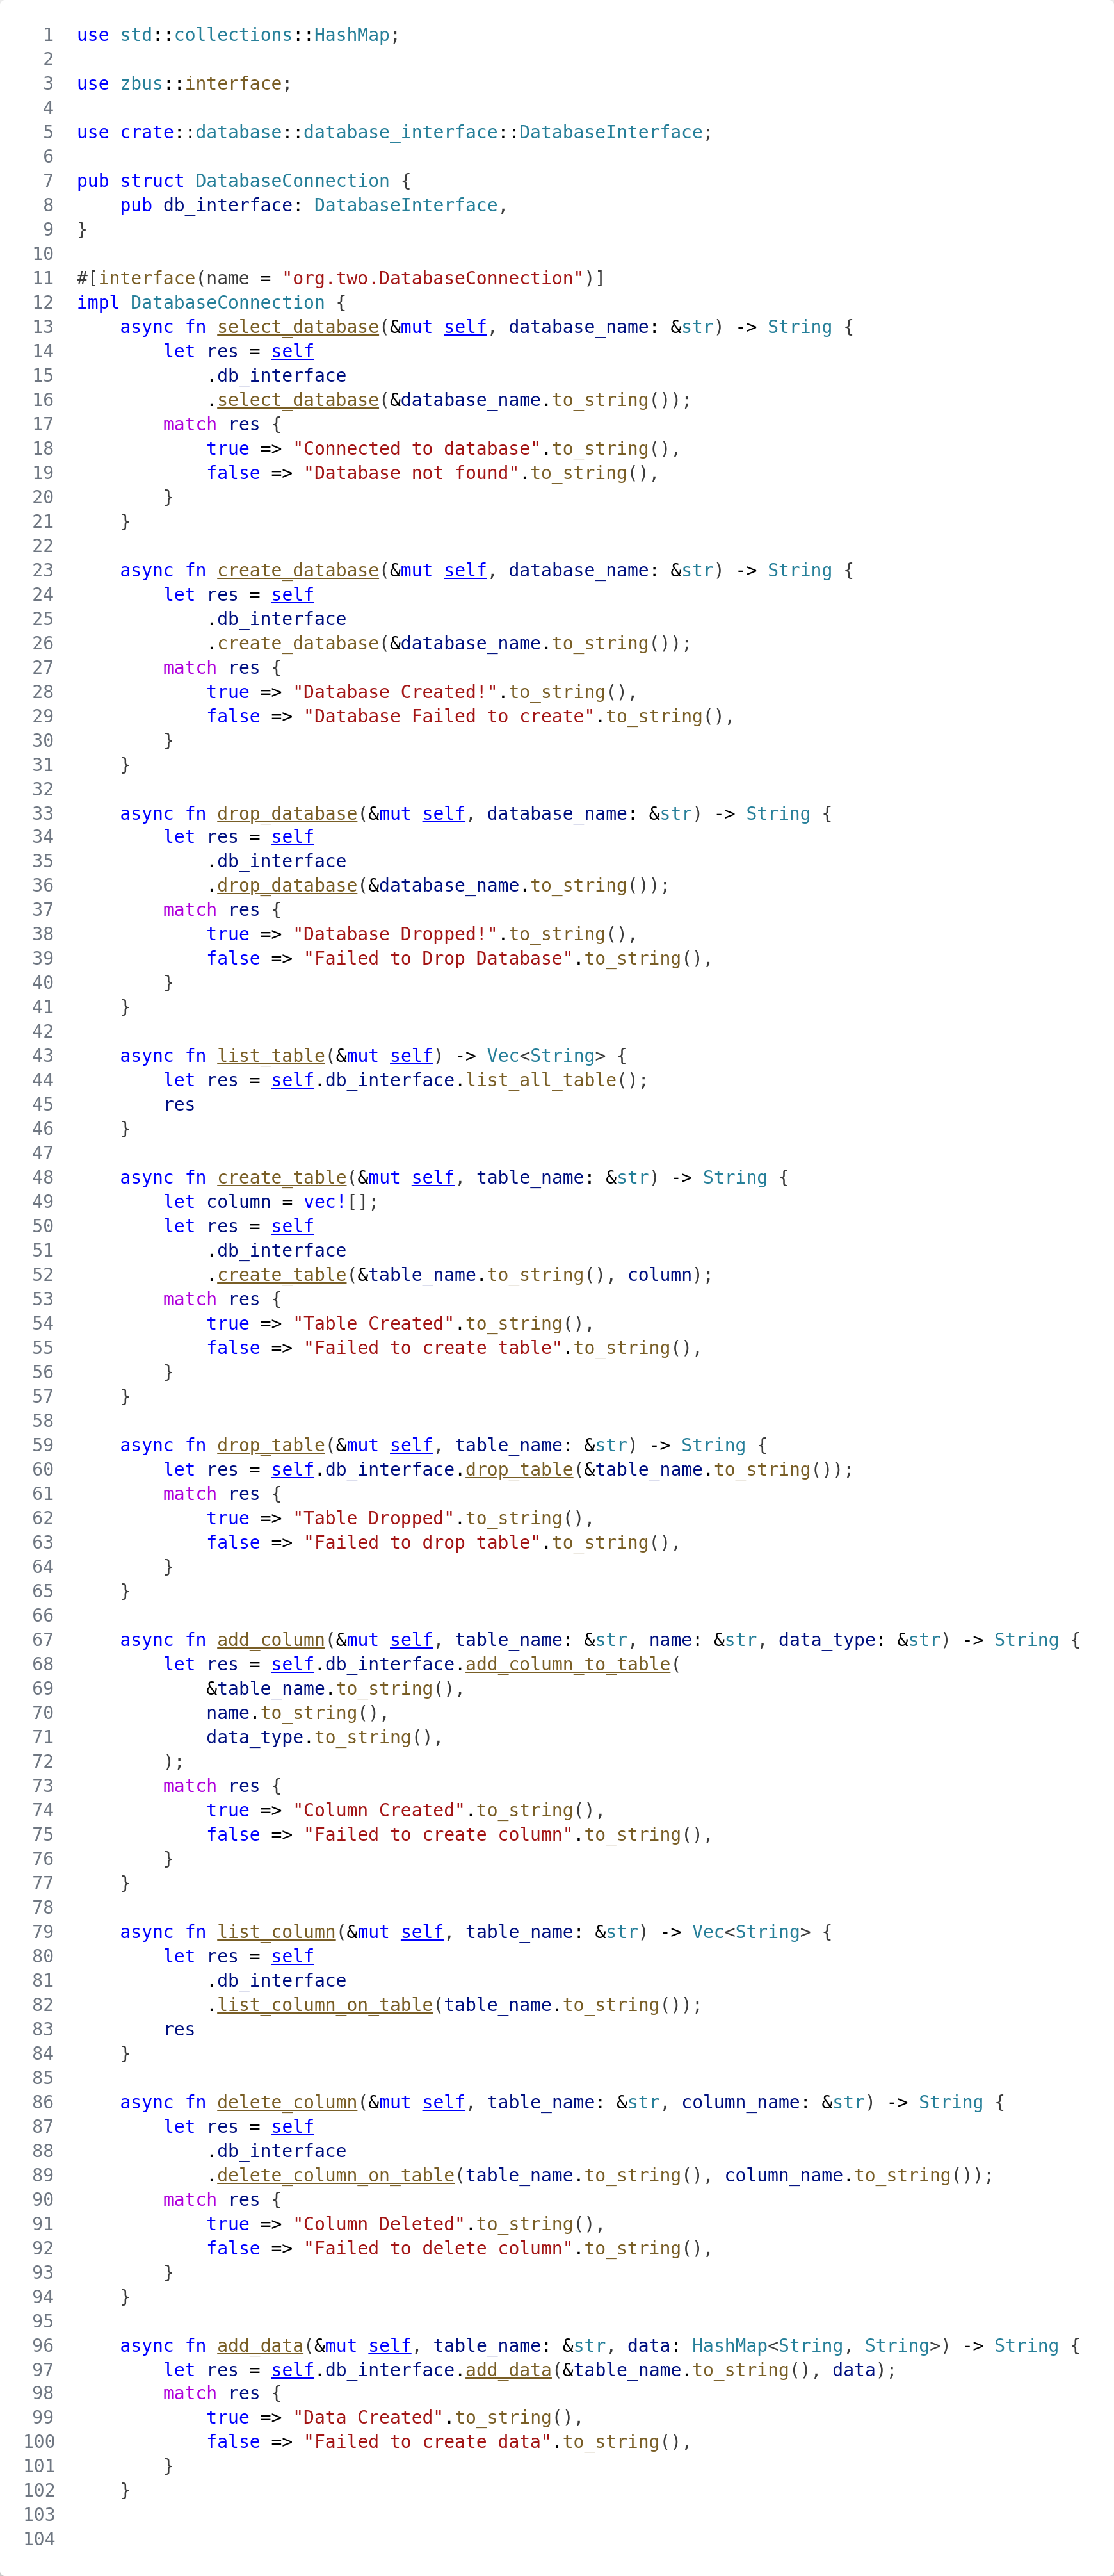
\includegraphics[width=0.6\textwidth]{gambar/lampiran/file-database-connection-1.png}
  \caption{\emph{File} database\_connection.rs bagian 1}
\end{figure}

\begin{figure}[H]
  \centering{}
	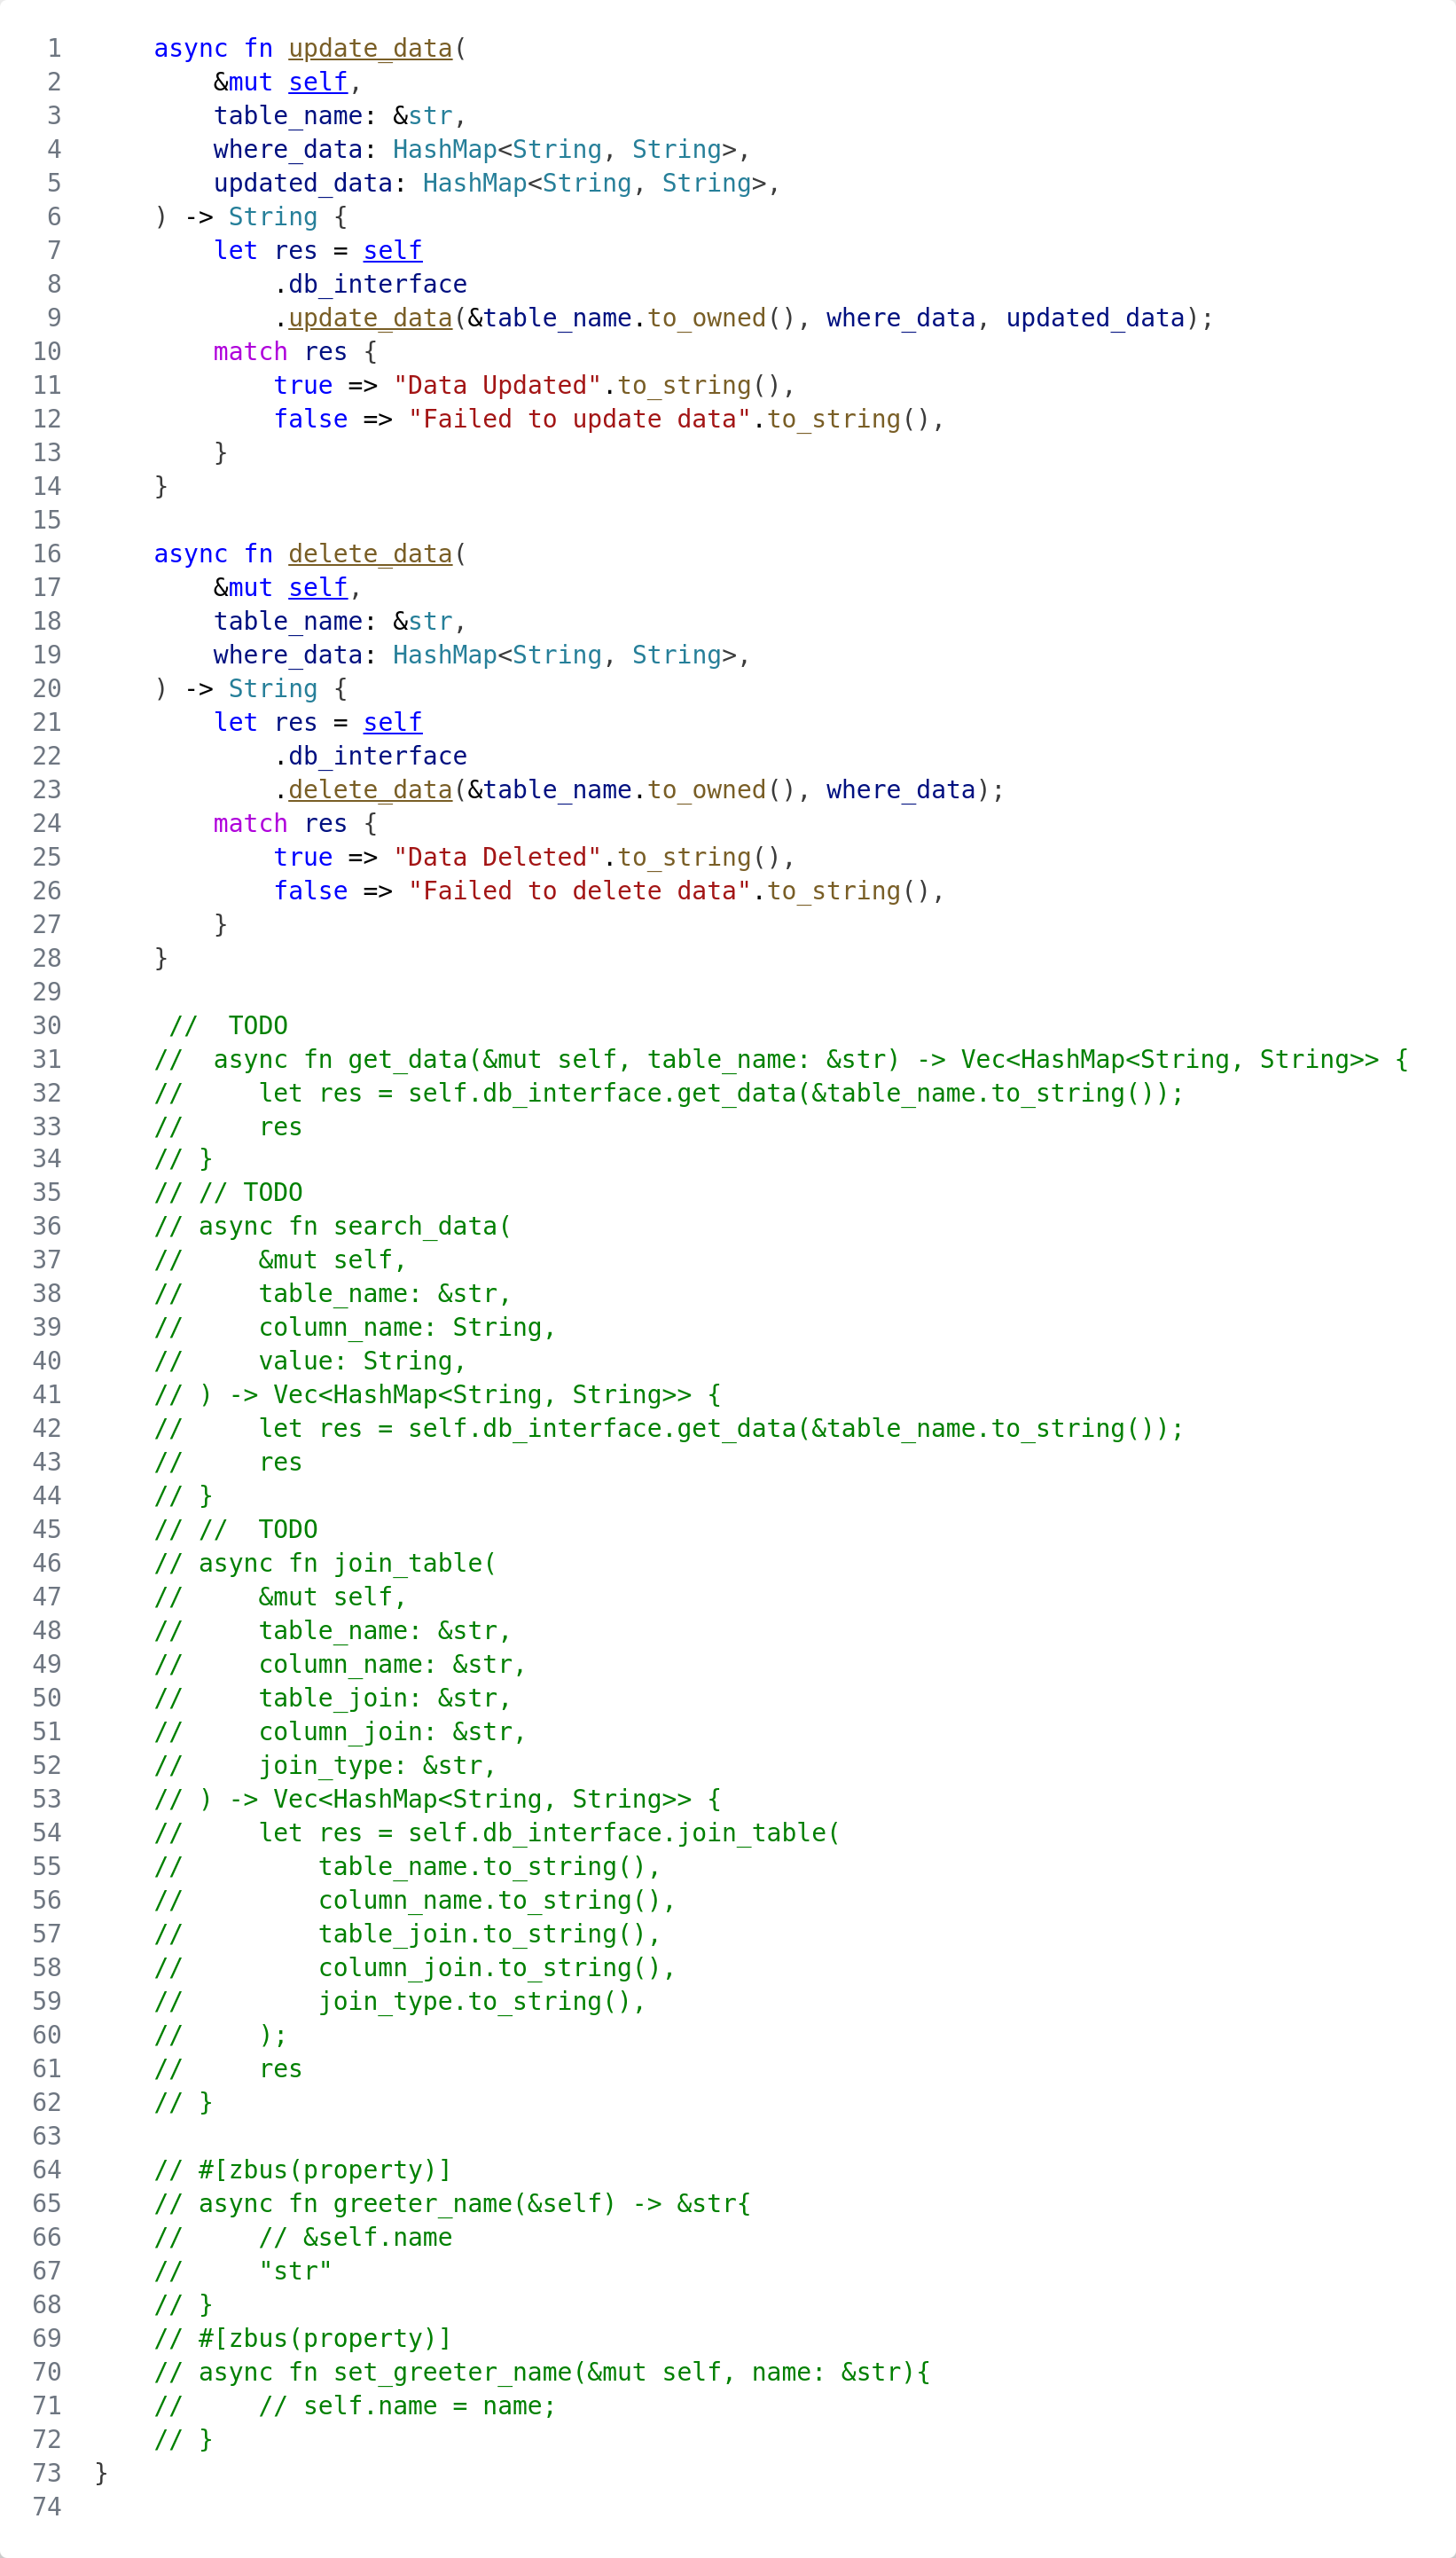
\includegraphics[width=0.7\textwidth]{gambar/lampiran/file-database-connection-2.png}
  \caption{\emph{File} database\_connection.rs bagian 2}
\end{figure}

\begin{figure}[H]
  \centering{}
	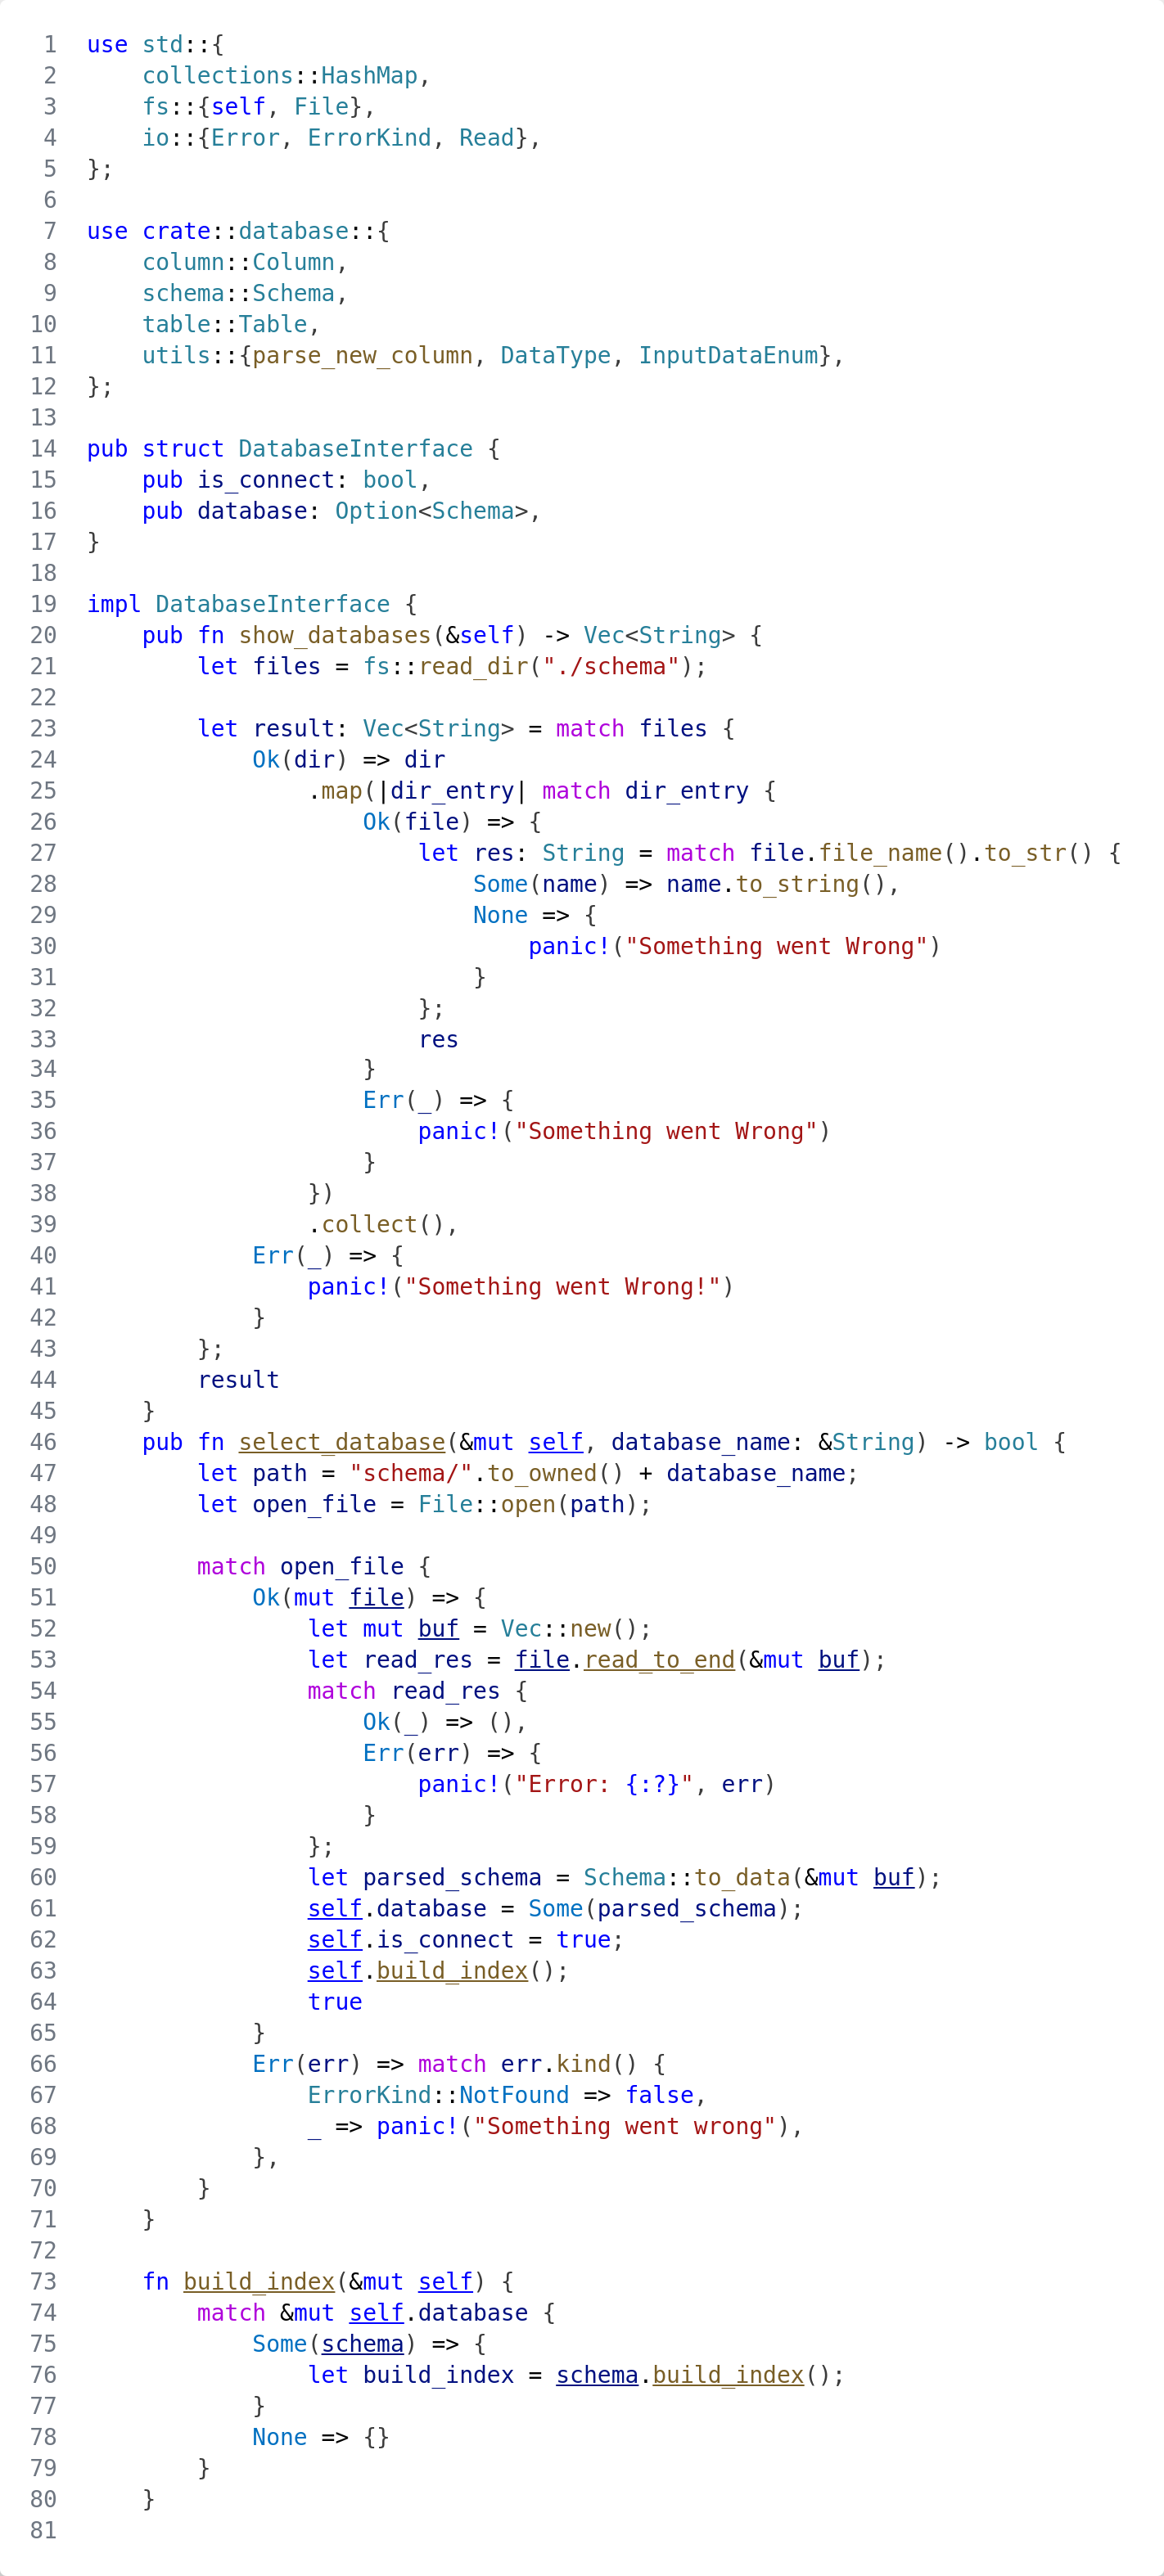
\includegraphics[width=0.6\textwidth]{gambar/lampiran/file-database-interface-1.png}
  \caption{\emph{File} database\_interface.rs bagian 1}
\end{figure}

\begin{figure}[H]
  \centering{}
	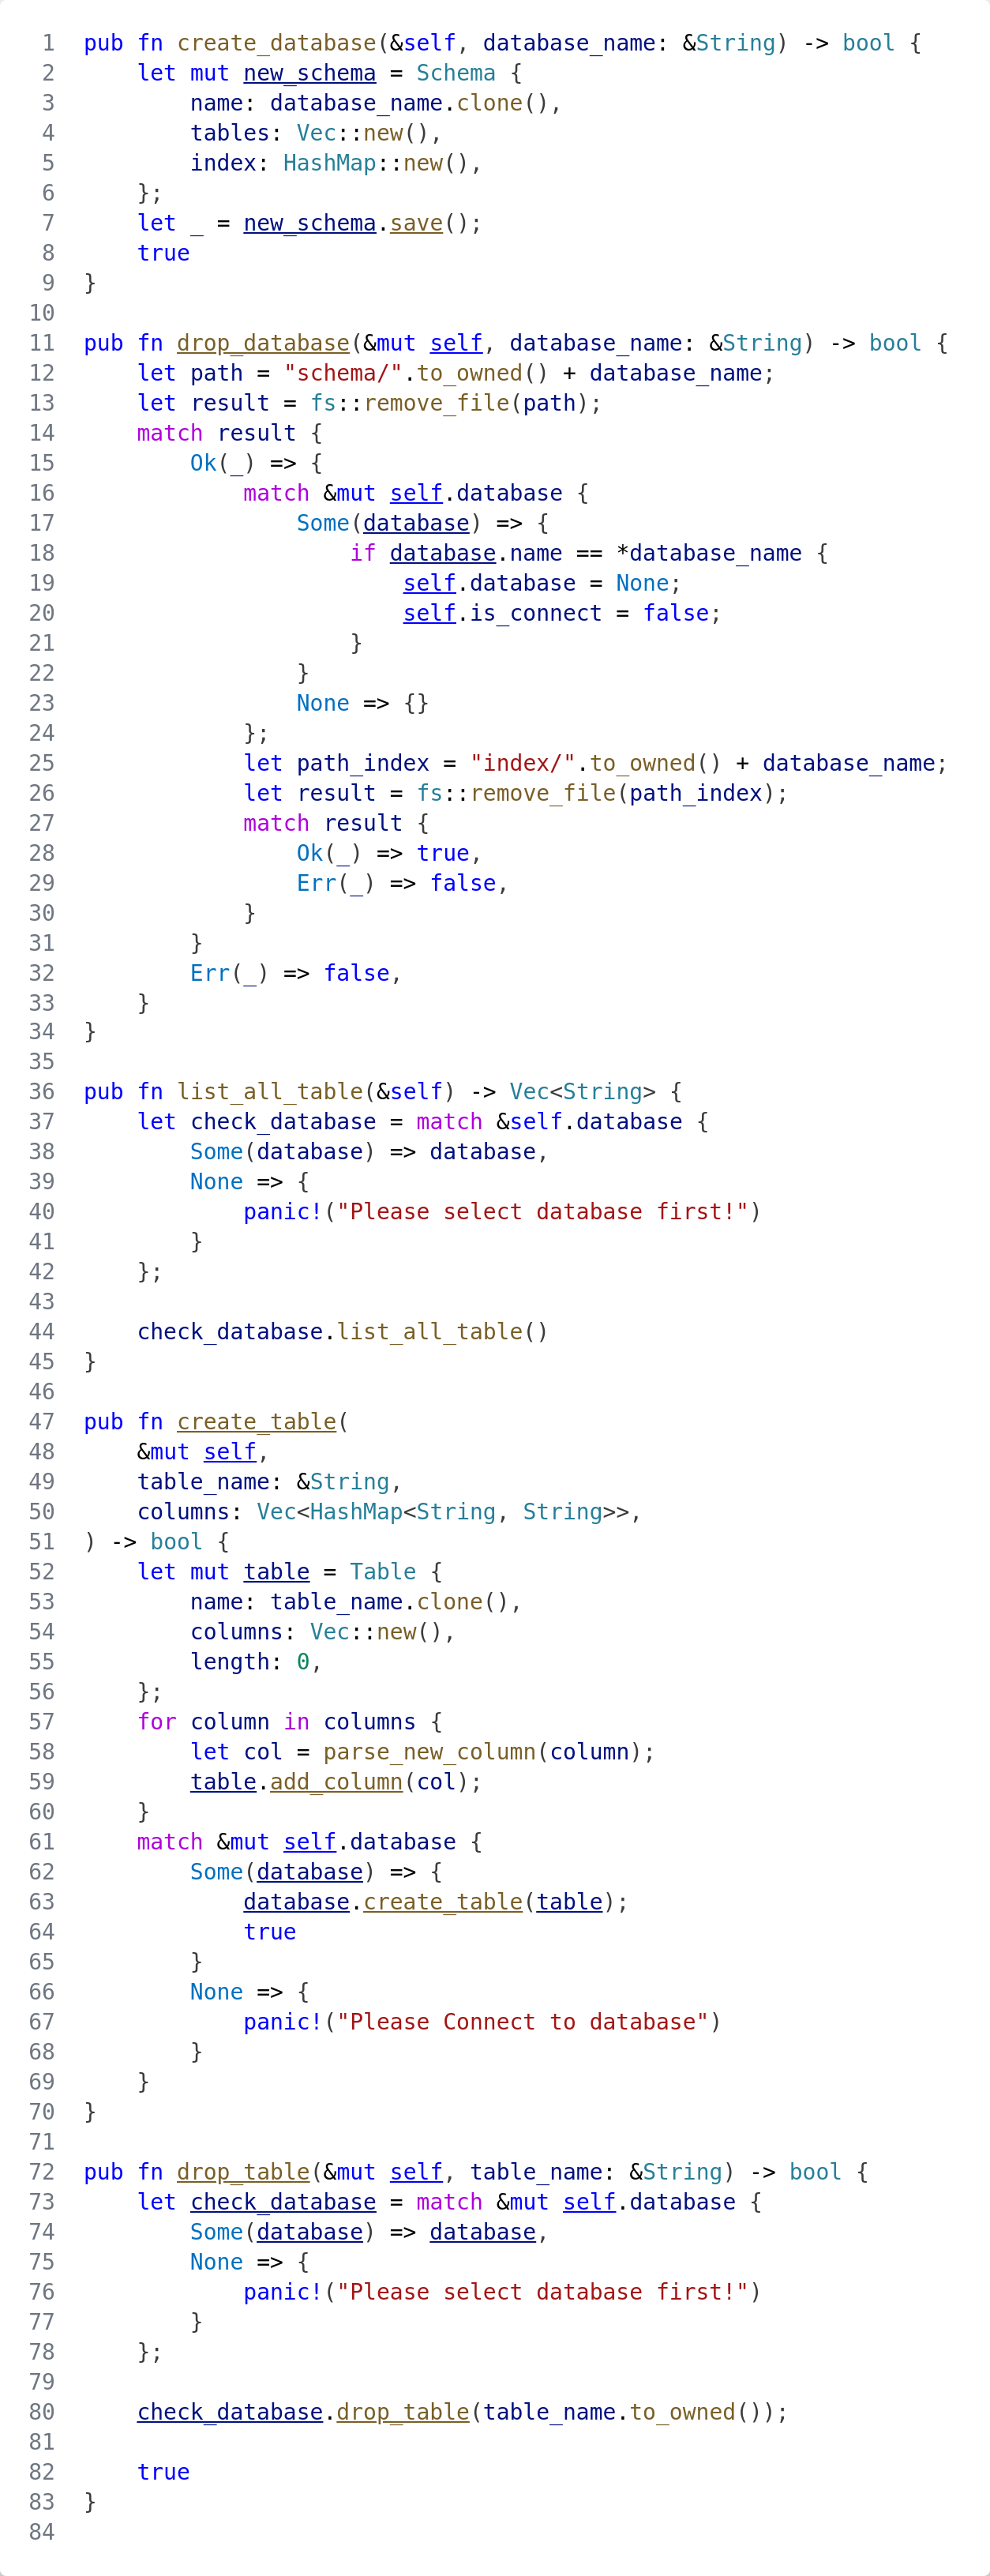
\includegraphics[width=0.4\textwidth]{gambar/lampiran/file-database-interface-2.png}
  \caption{\emph{File} database\_interface.rs bagian 2}
\end{figure}

\begin{figure}[H]
  \centering{}
	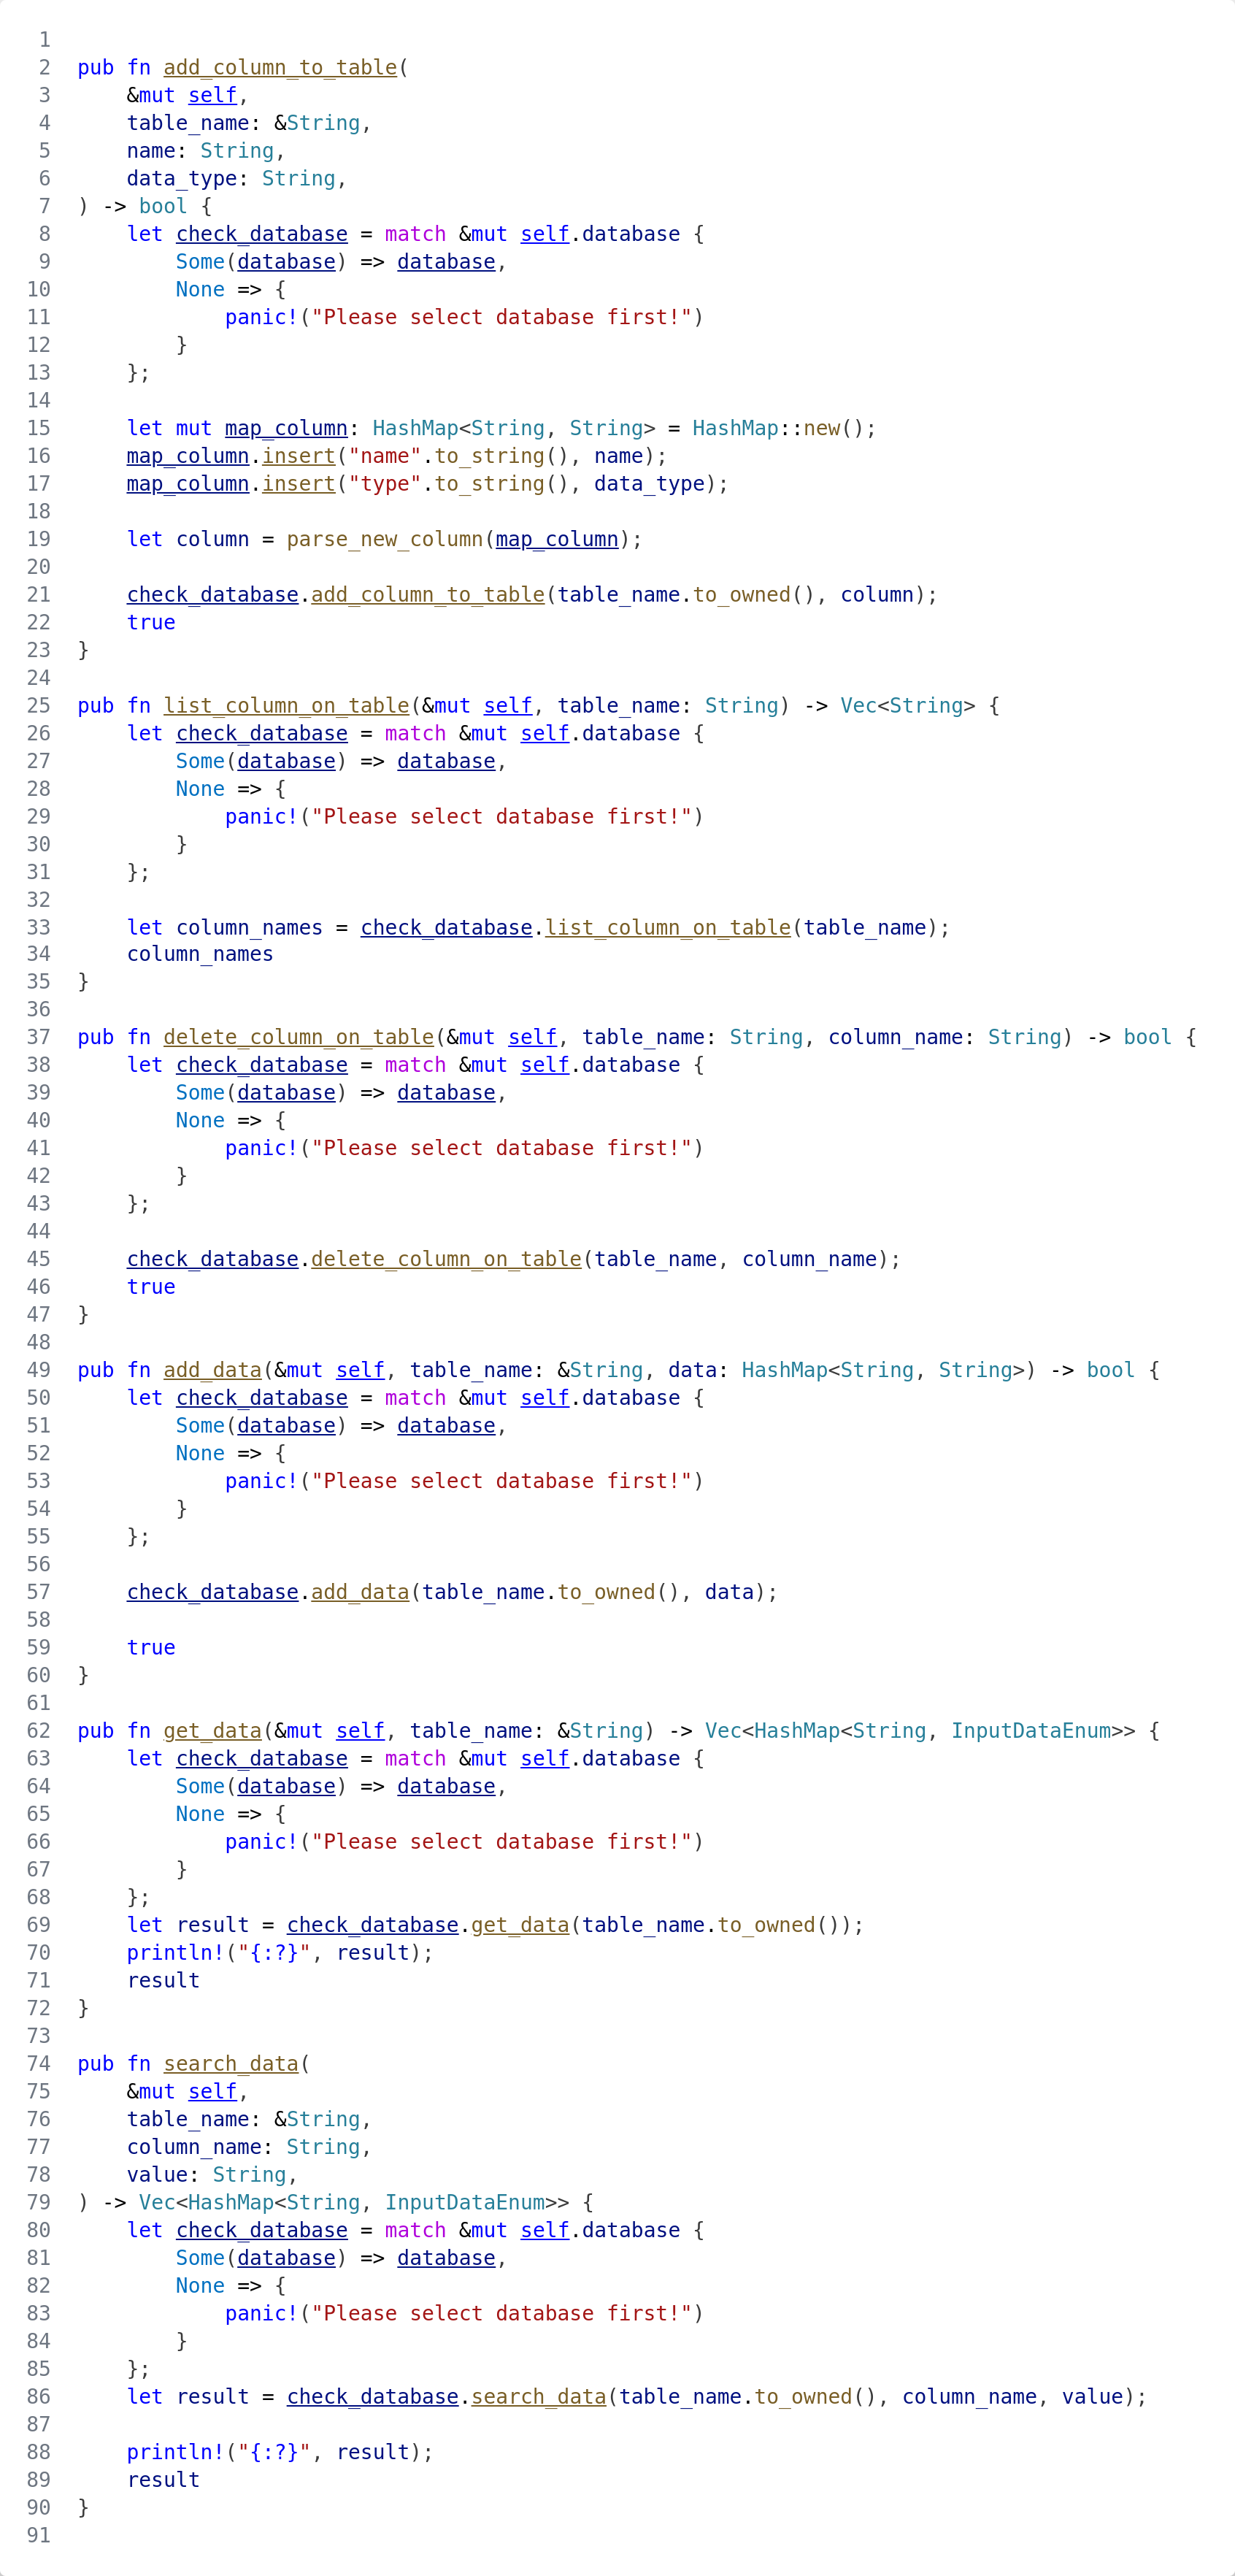
\includegraphics[width=0.6\textwidth]{gambar/lampiran/file-database-interface-3.png}
  \caption{\emph{File} database\_interface.rs bagian 3}
\end{figure}

\begin{figure}[H]
  \centering{}
	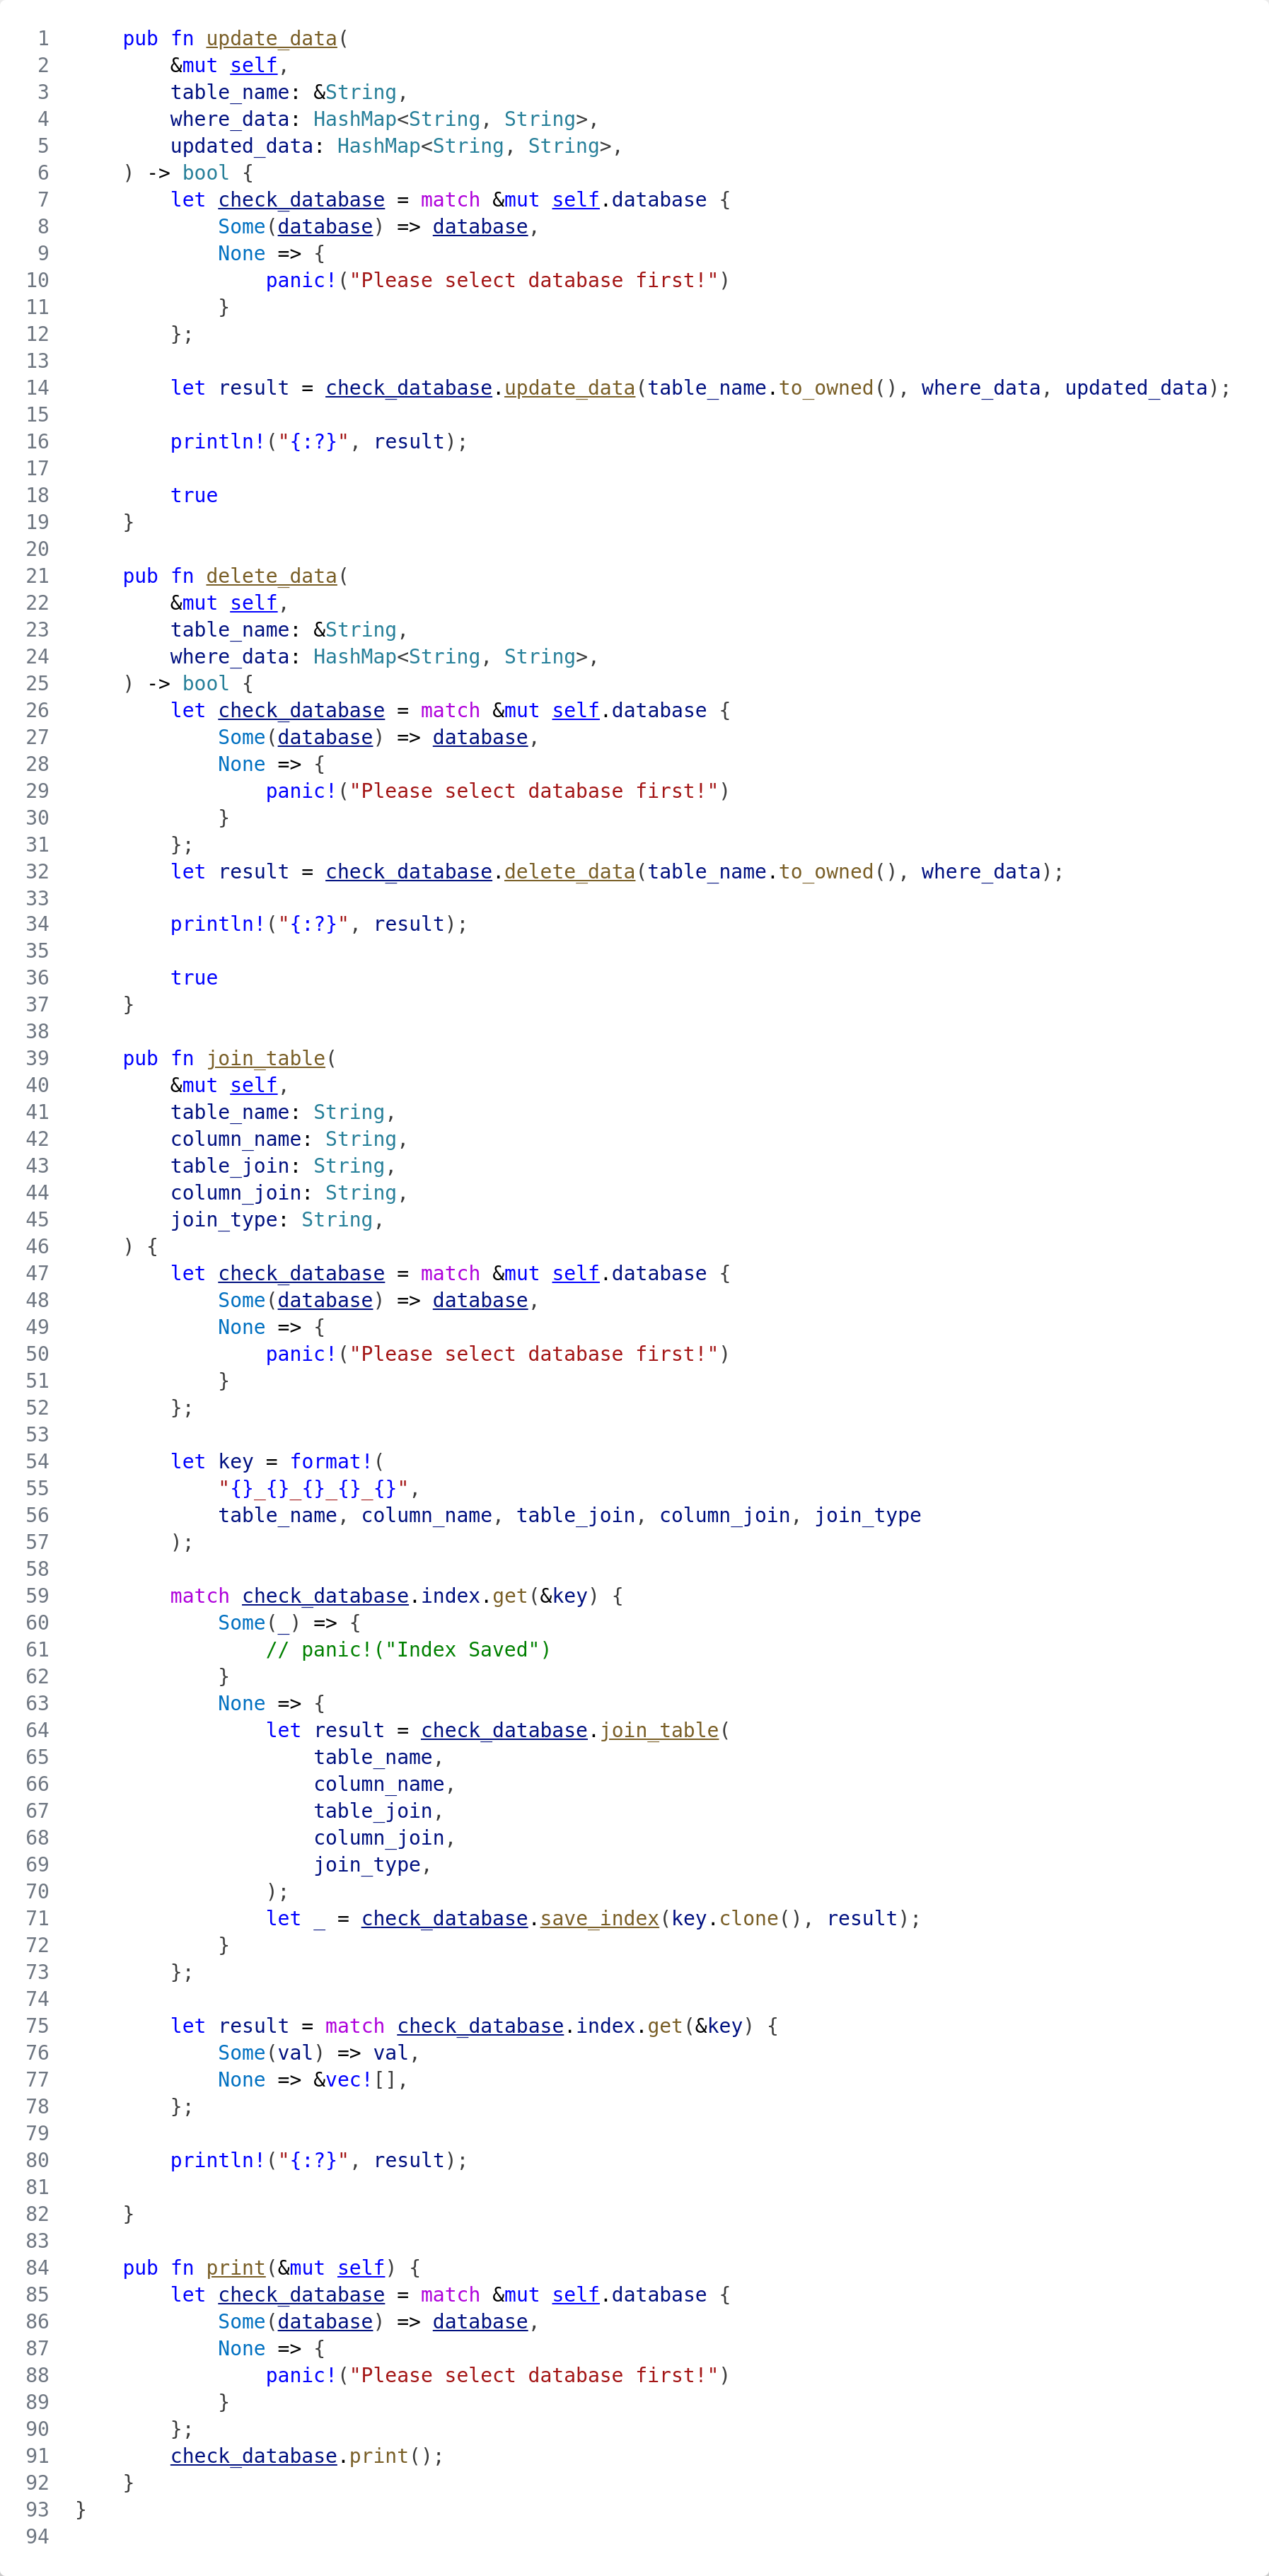
\includegraphics[width=0.6\textwidth]{gambar/lampiran/file-database-interface-4.png}
  \caption{\emph{File} database\_interface.rs bagian 4}
\end{figure}


\begin{figure}[H]
  \centering{}
	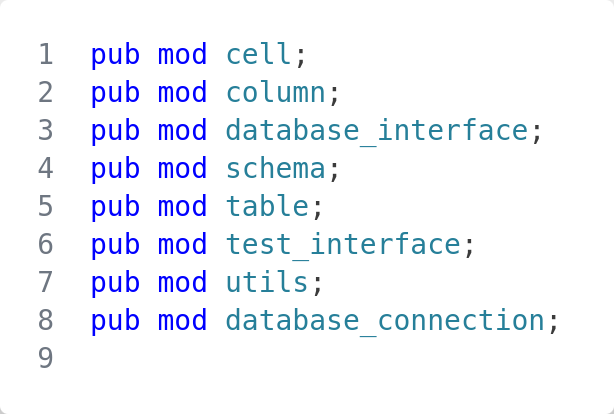
\includegraphics[width=0.9\textwidth]{gambar/lampiran/file-mod.png}
  \caption{\emph{File} mod}
\end{figure}


\begin{figure}[H]
  \centering{}
	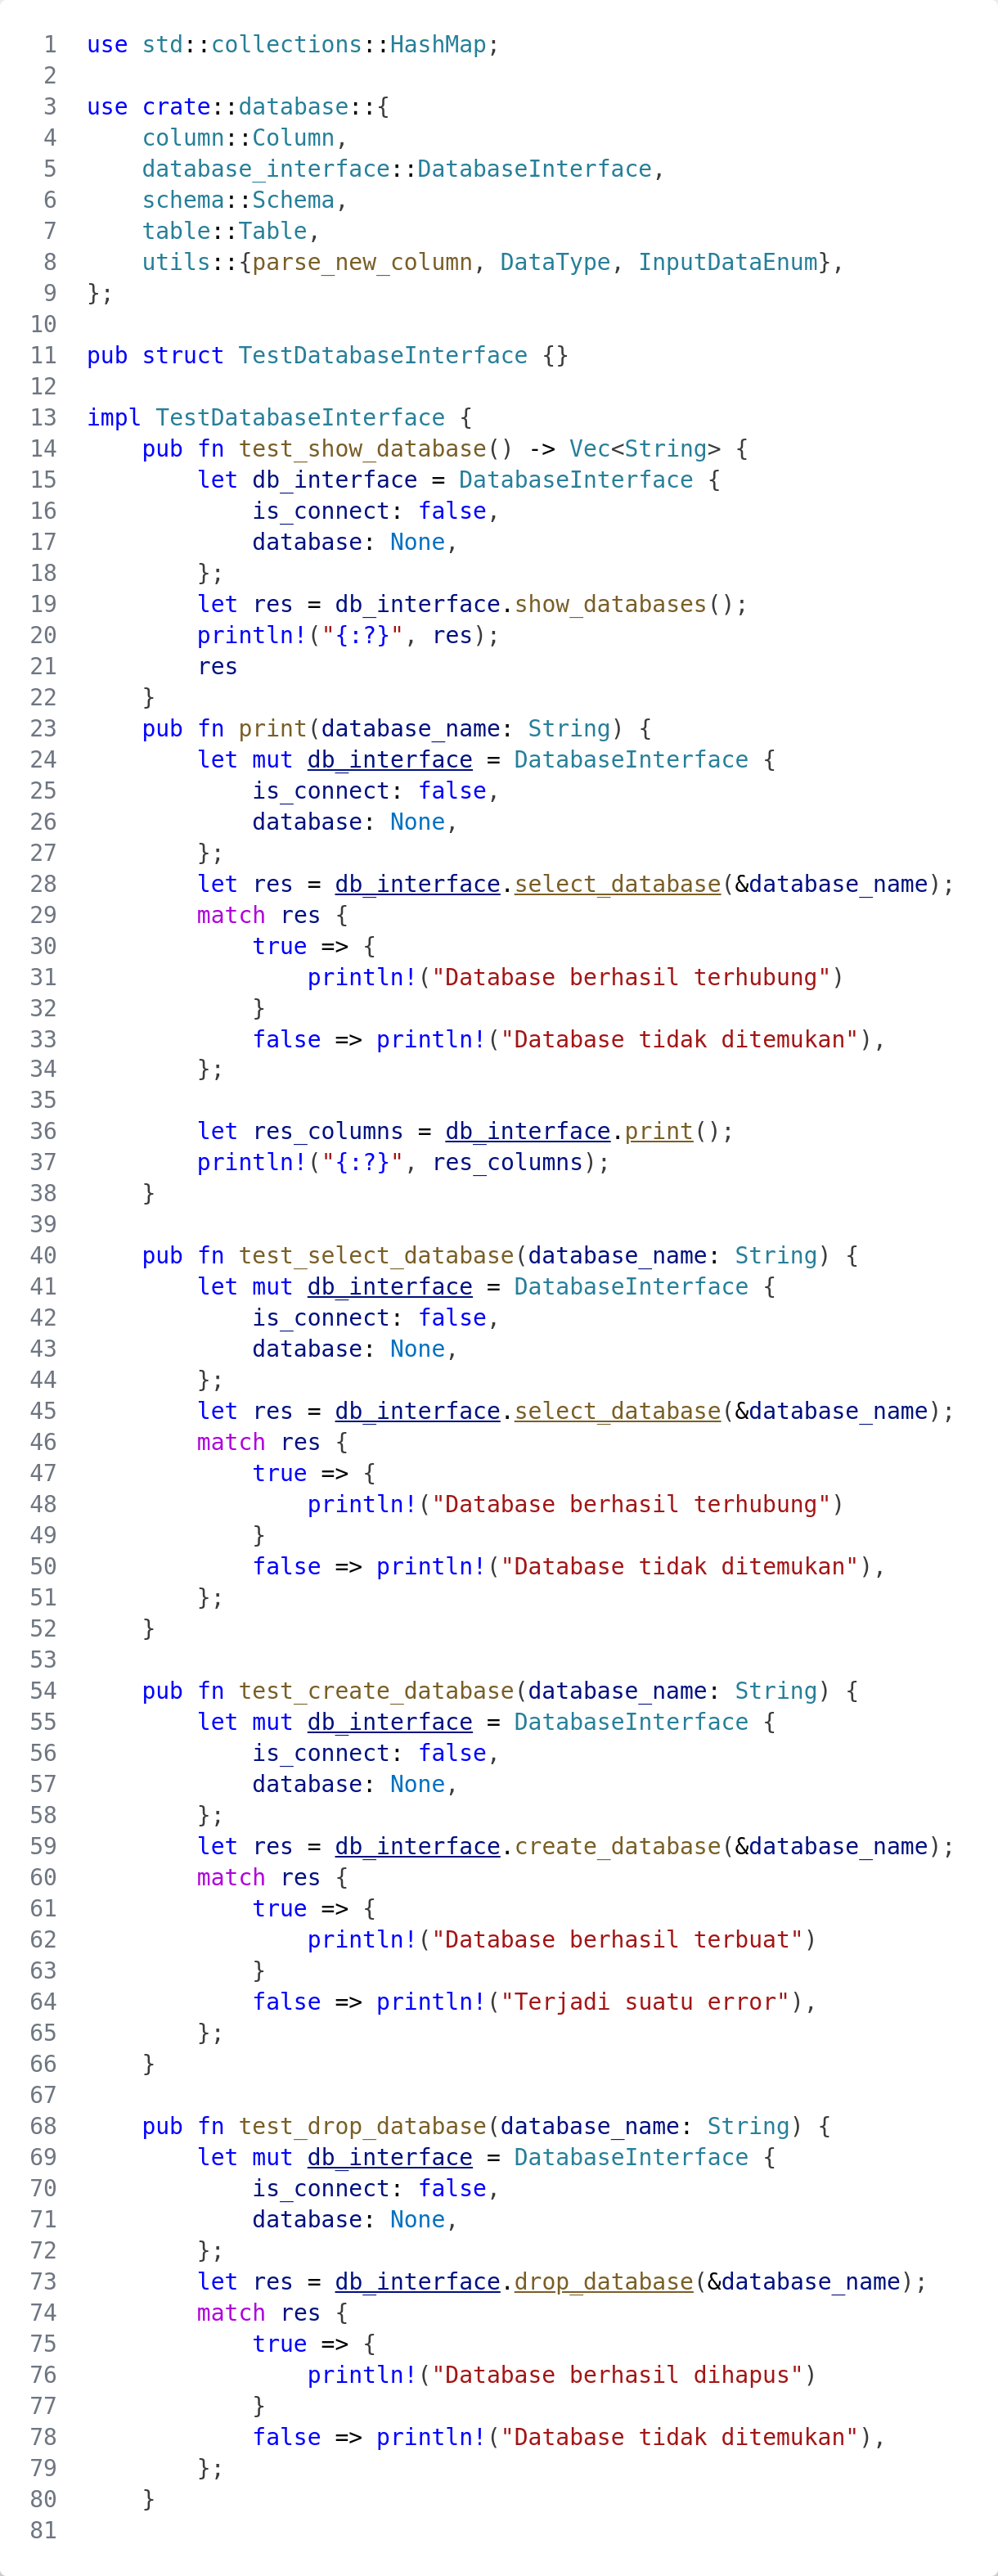
\includegraphics[width=0.3\textwidth]{gambar/lampiran/file-test-database-interface-1.png}
  \caption{\emph{File} test\_interface.rs bagian 1}
\end{figure}

\begin{figure}[H]
  \centering{}
	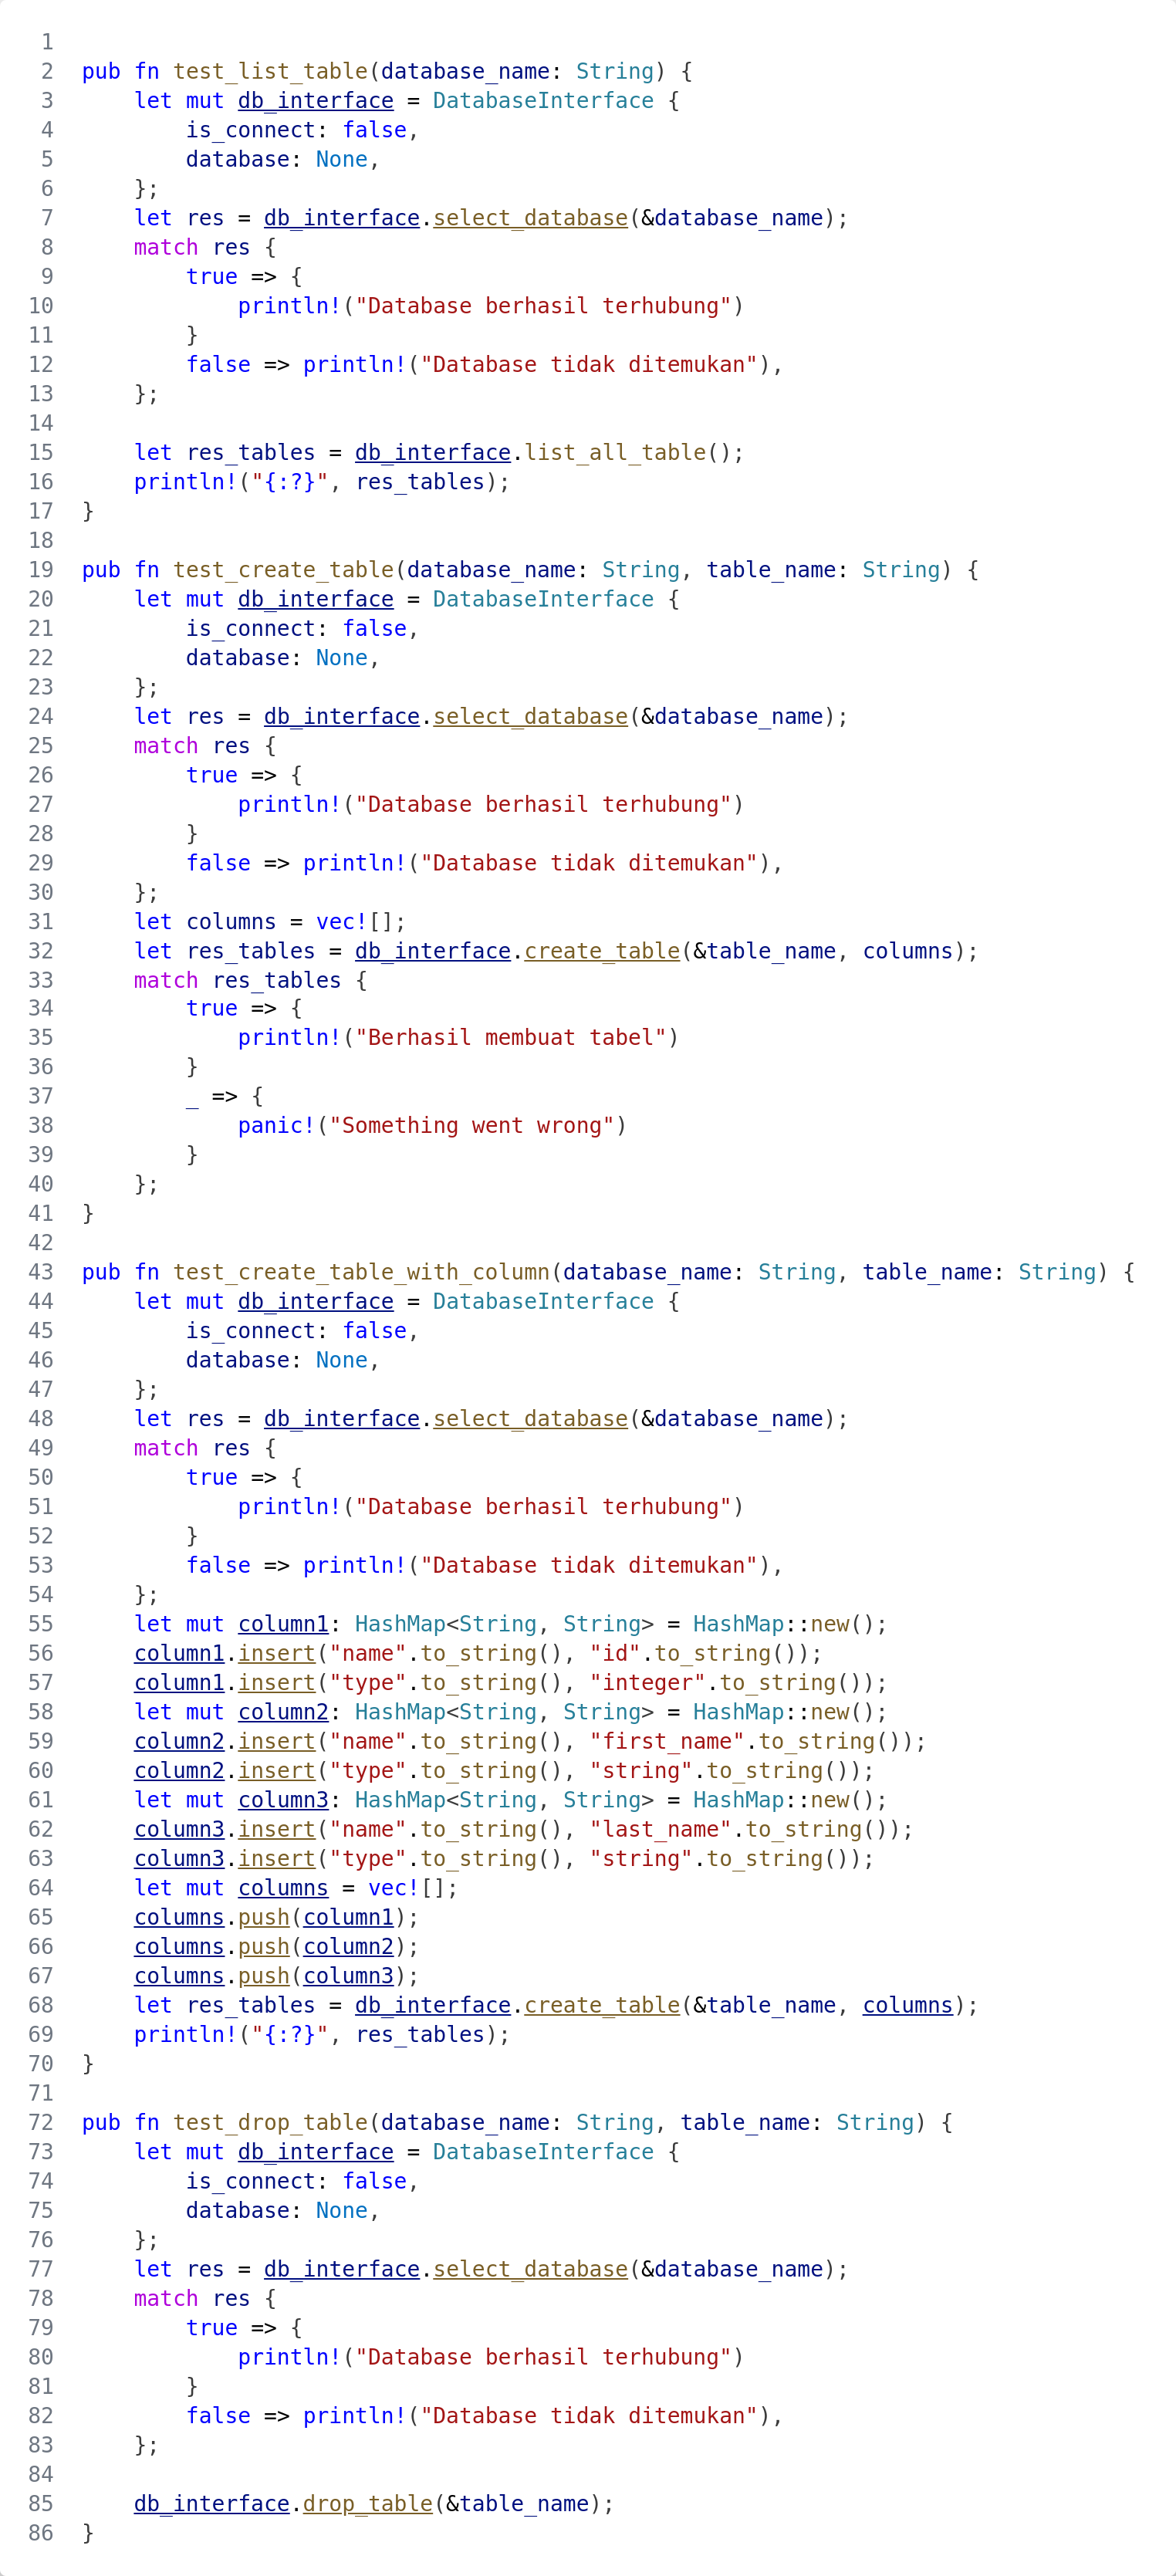
\includegraphics[width=0.4\textwidth]{gambar/lampiran/file-test-database-interface-2.png}
  \caption{\emph{File} test\_interface.rs bagian 2}
\end{figure}

\begin{figure}[H]
  \centering{}
	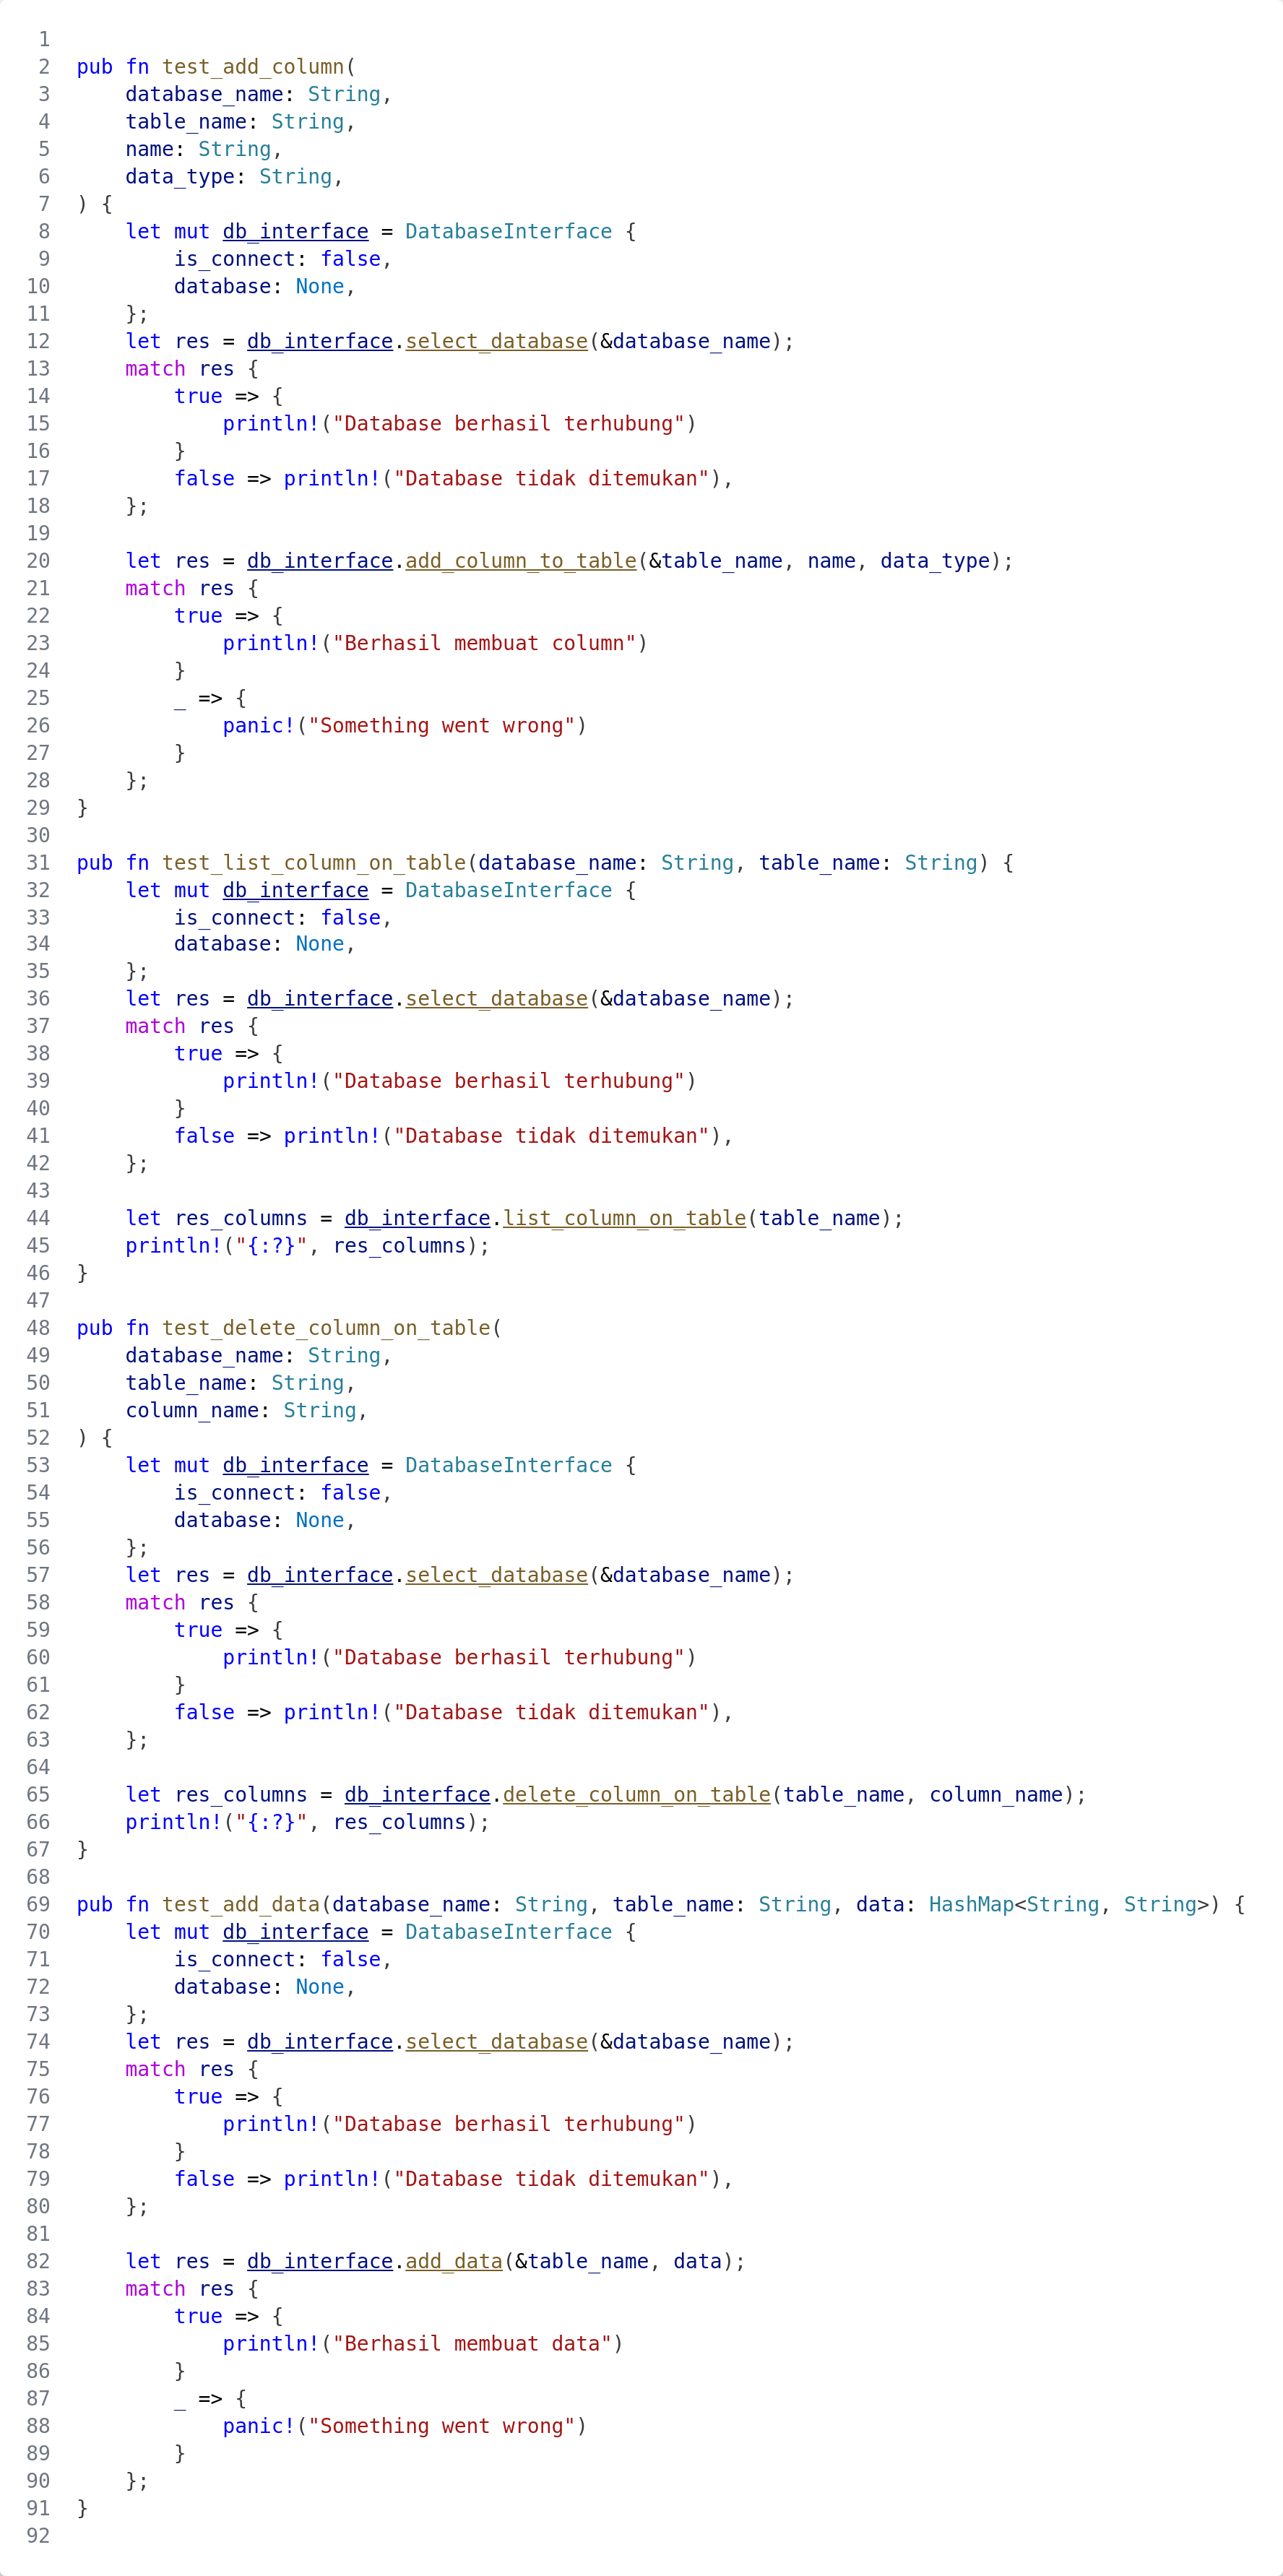
\includegraphics[width=0.6\textwidth]{gambar/lampiran/file-test-database-interface-3.png}
  \caption{\emph{File} test\_interface.rs bagian 3}
\end{figure}

\begin{figure}[H]
  \centering{}
	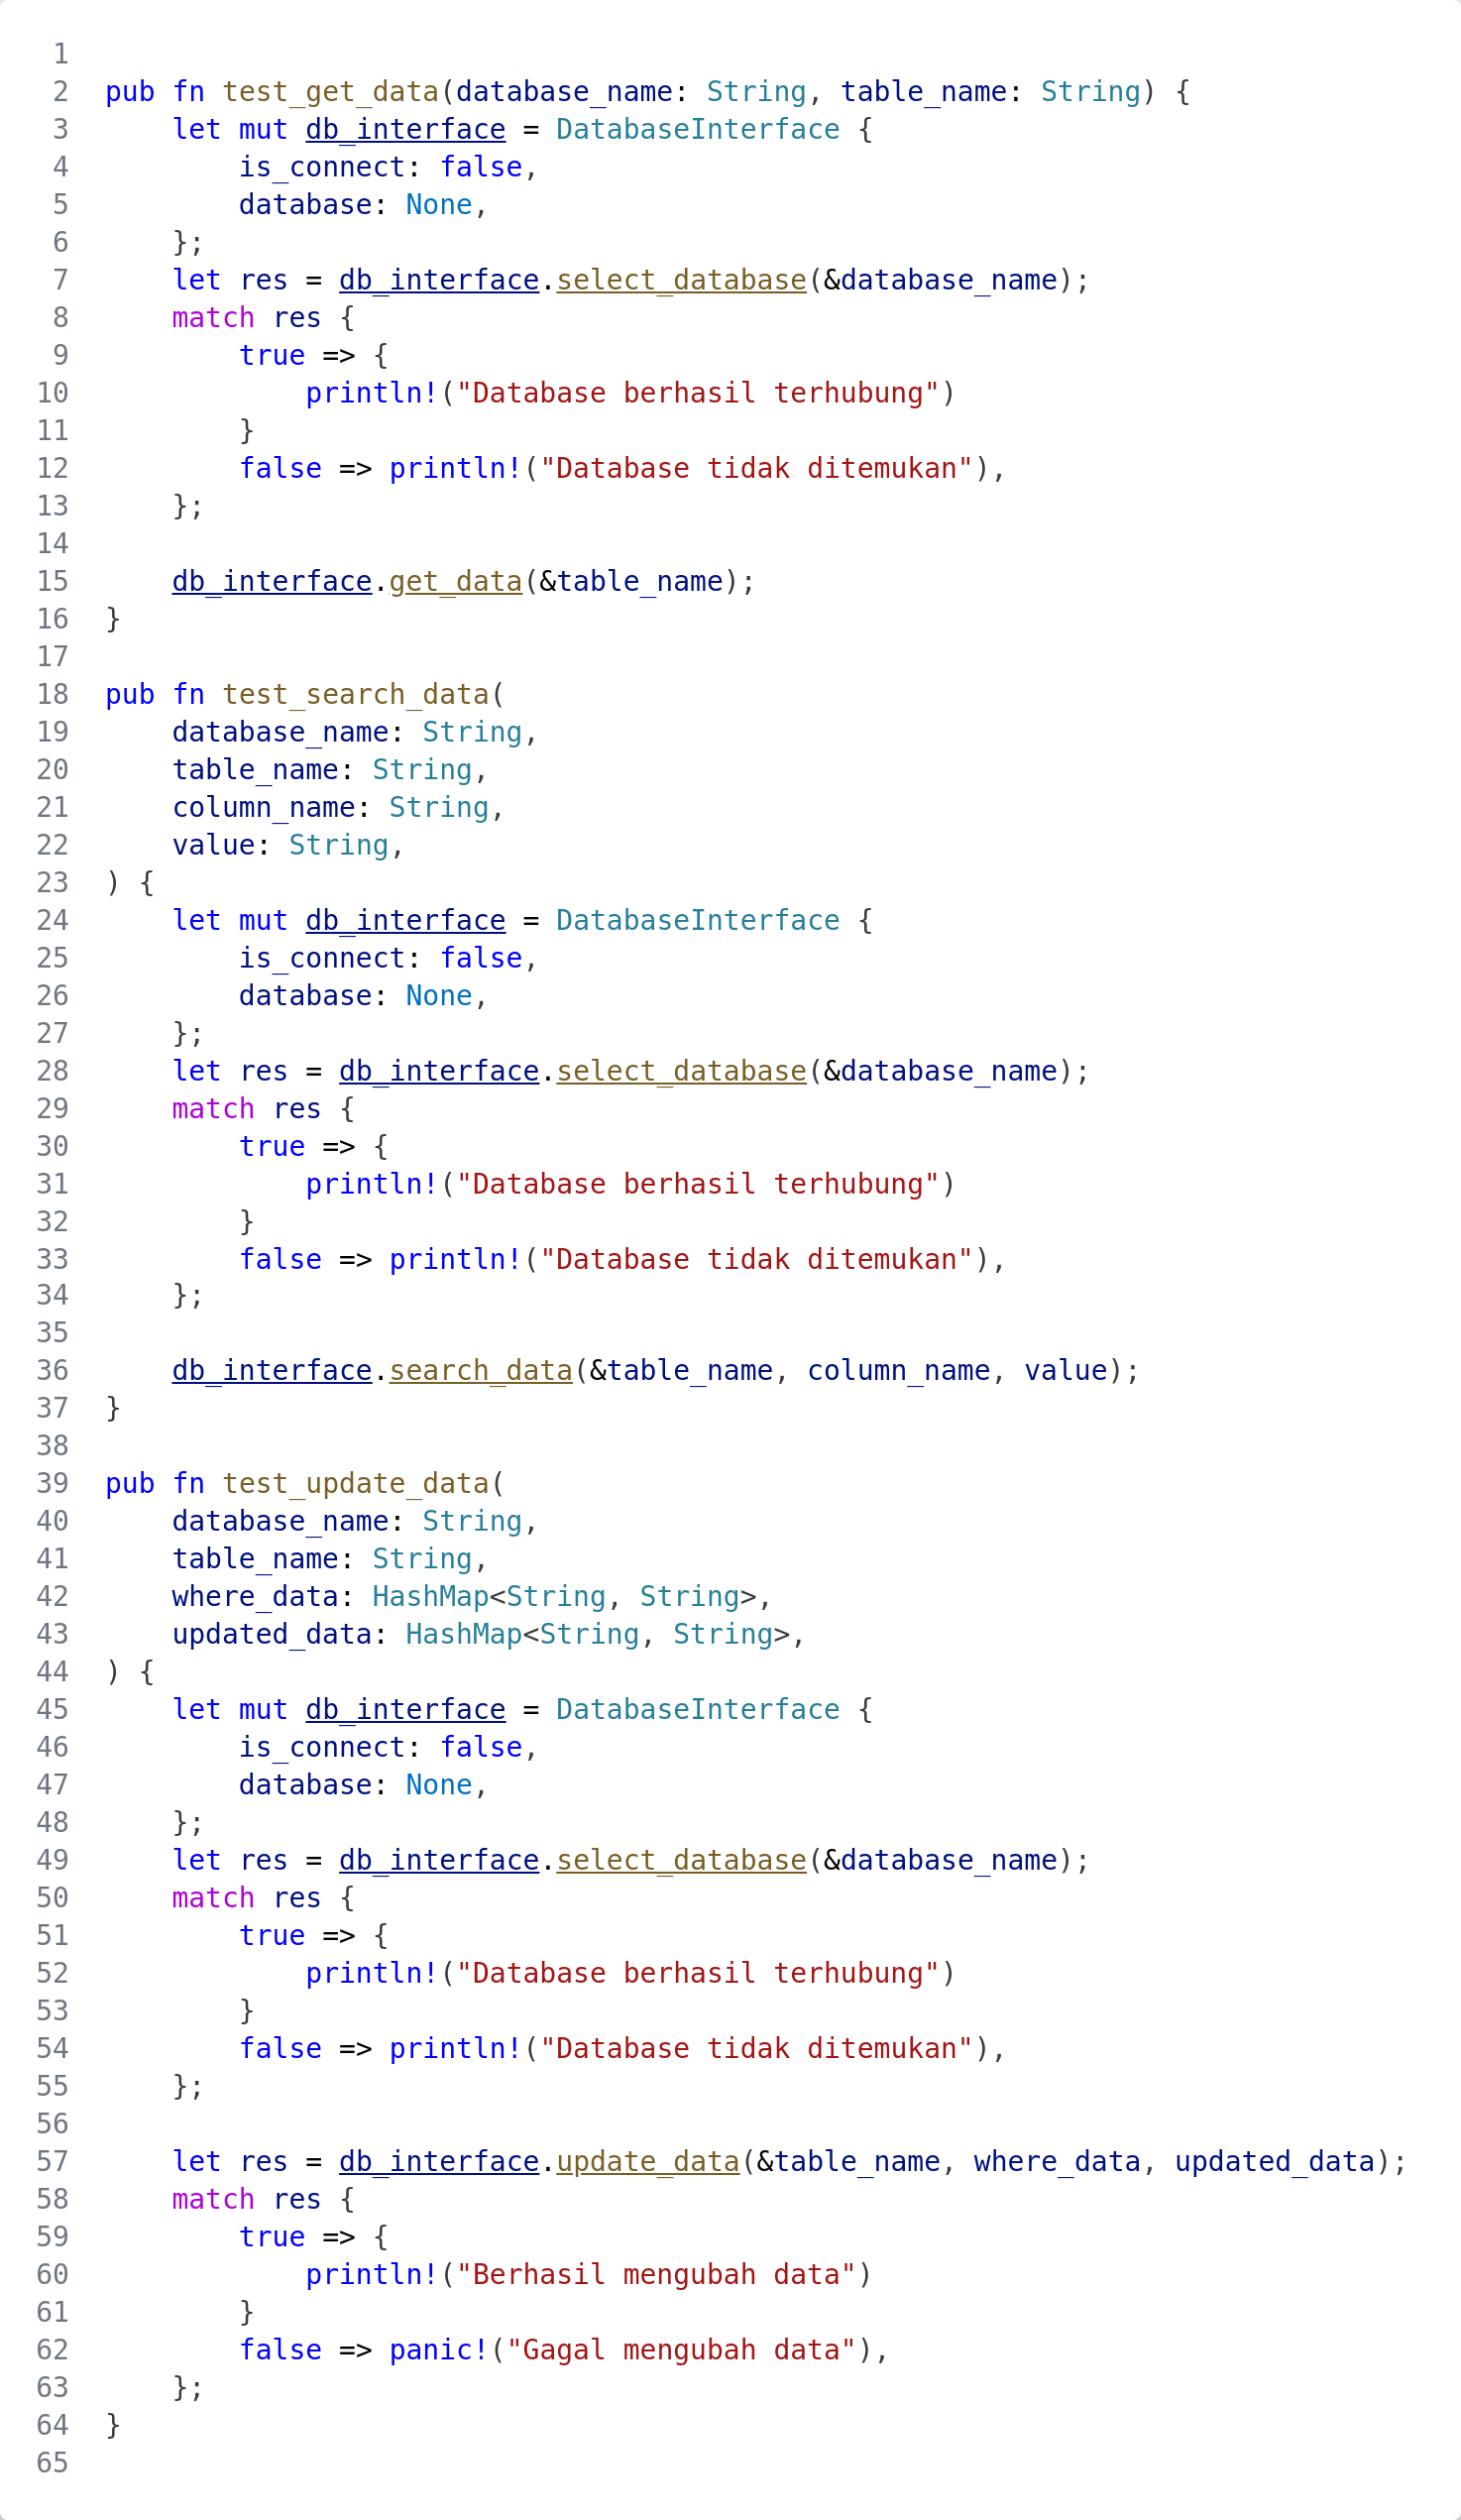
\includegraphics[width=0.6\textwidth]{gambar/lampiran/file-test-database-interface-4.png}
  \caption{\emph{File} test\_interface.rs bagian 4}
\end{figure}

\begin{figure}[H]
  \centering{}
	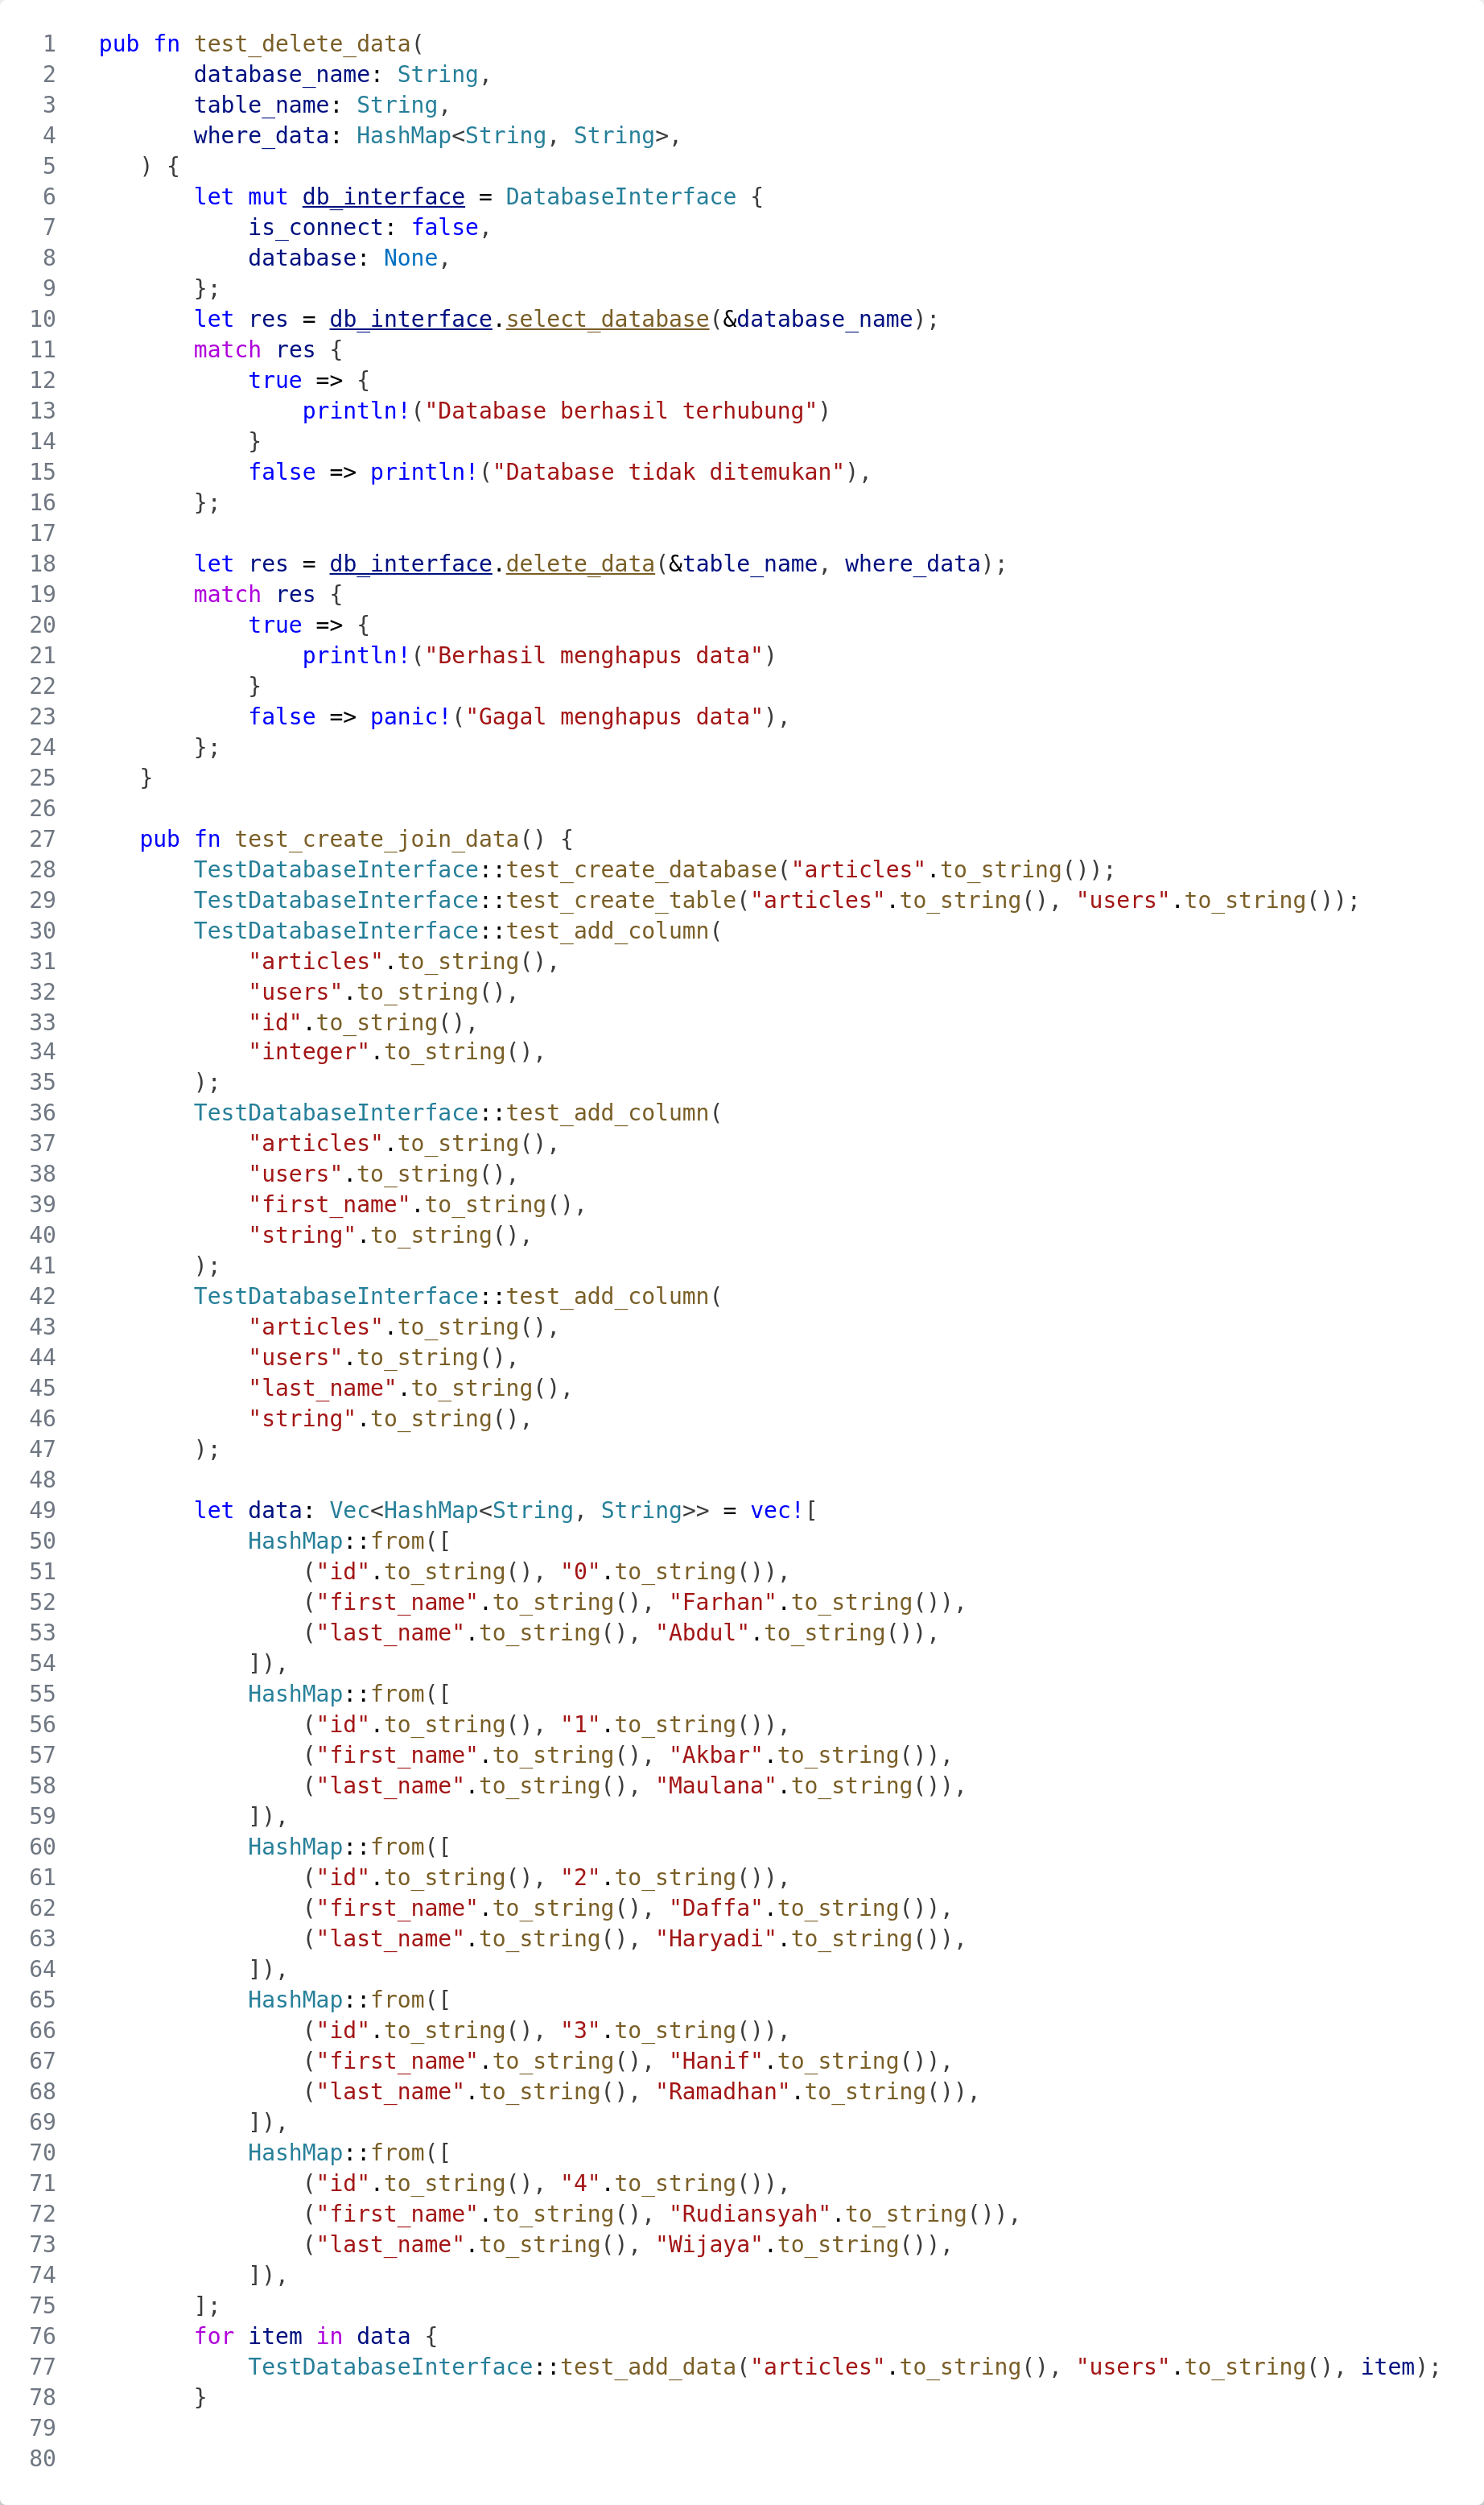
\includegraphics[width=0.6\textwidth]{gambar/lampiran/file-test-database-interface-5.png}
  \caption{\emph{File} test\_interface.rs bagian 5}
\end{figure}

\begin{figure}[H]
  \centering{}
	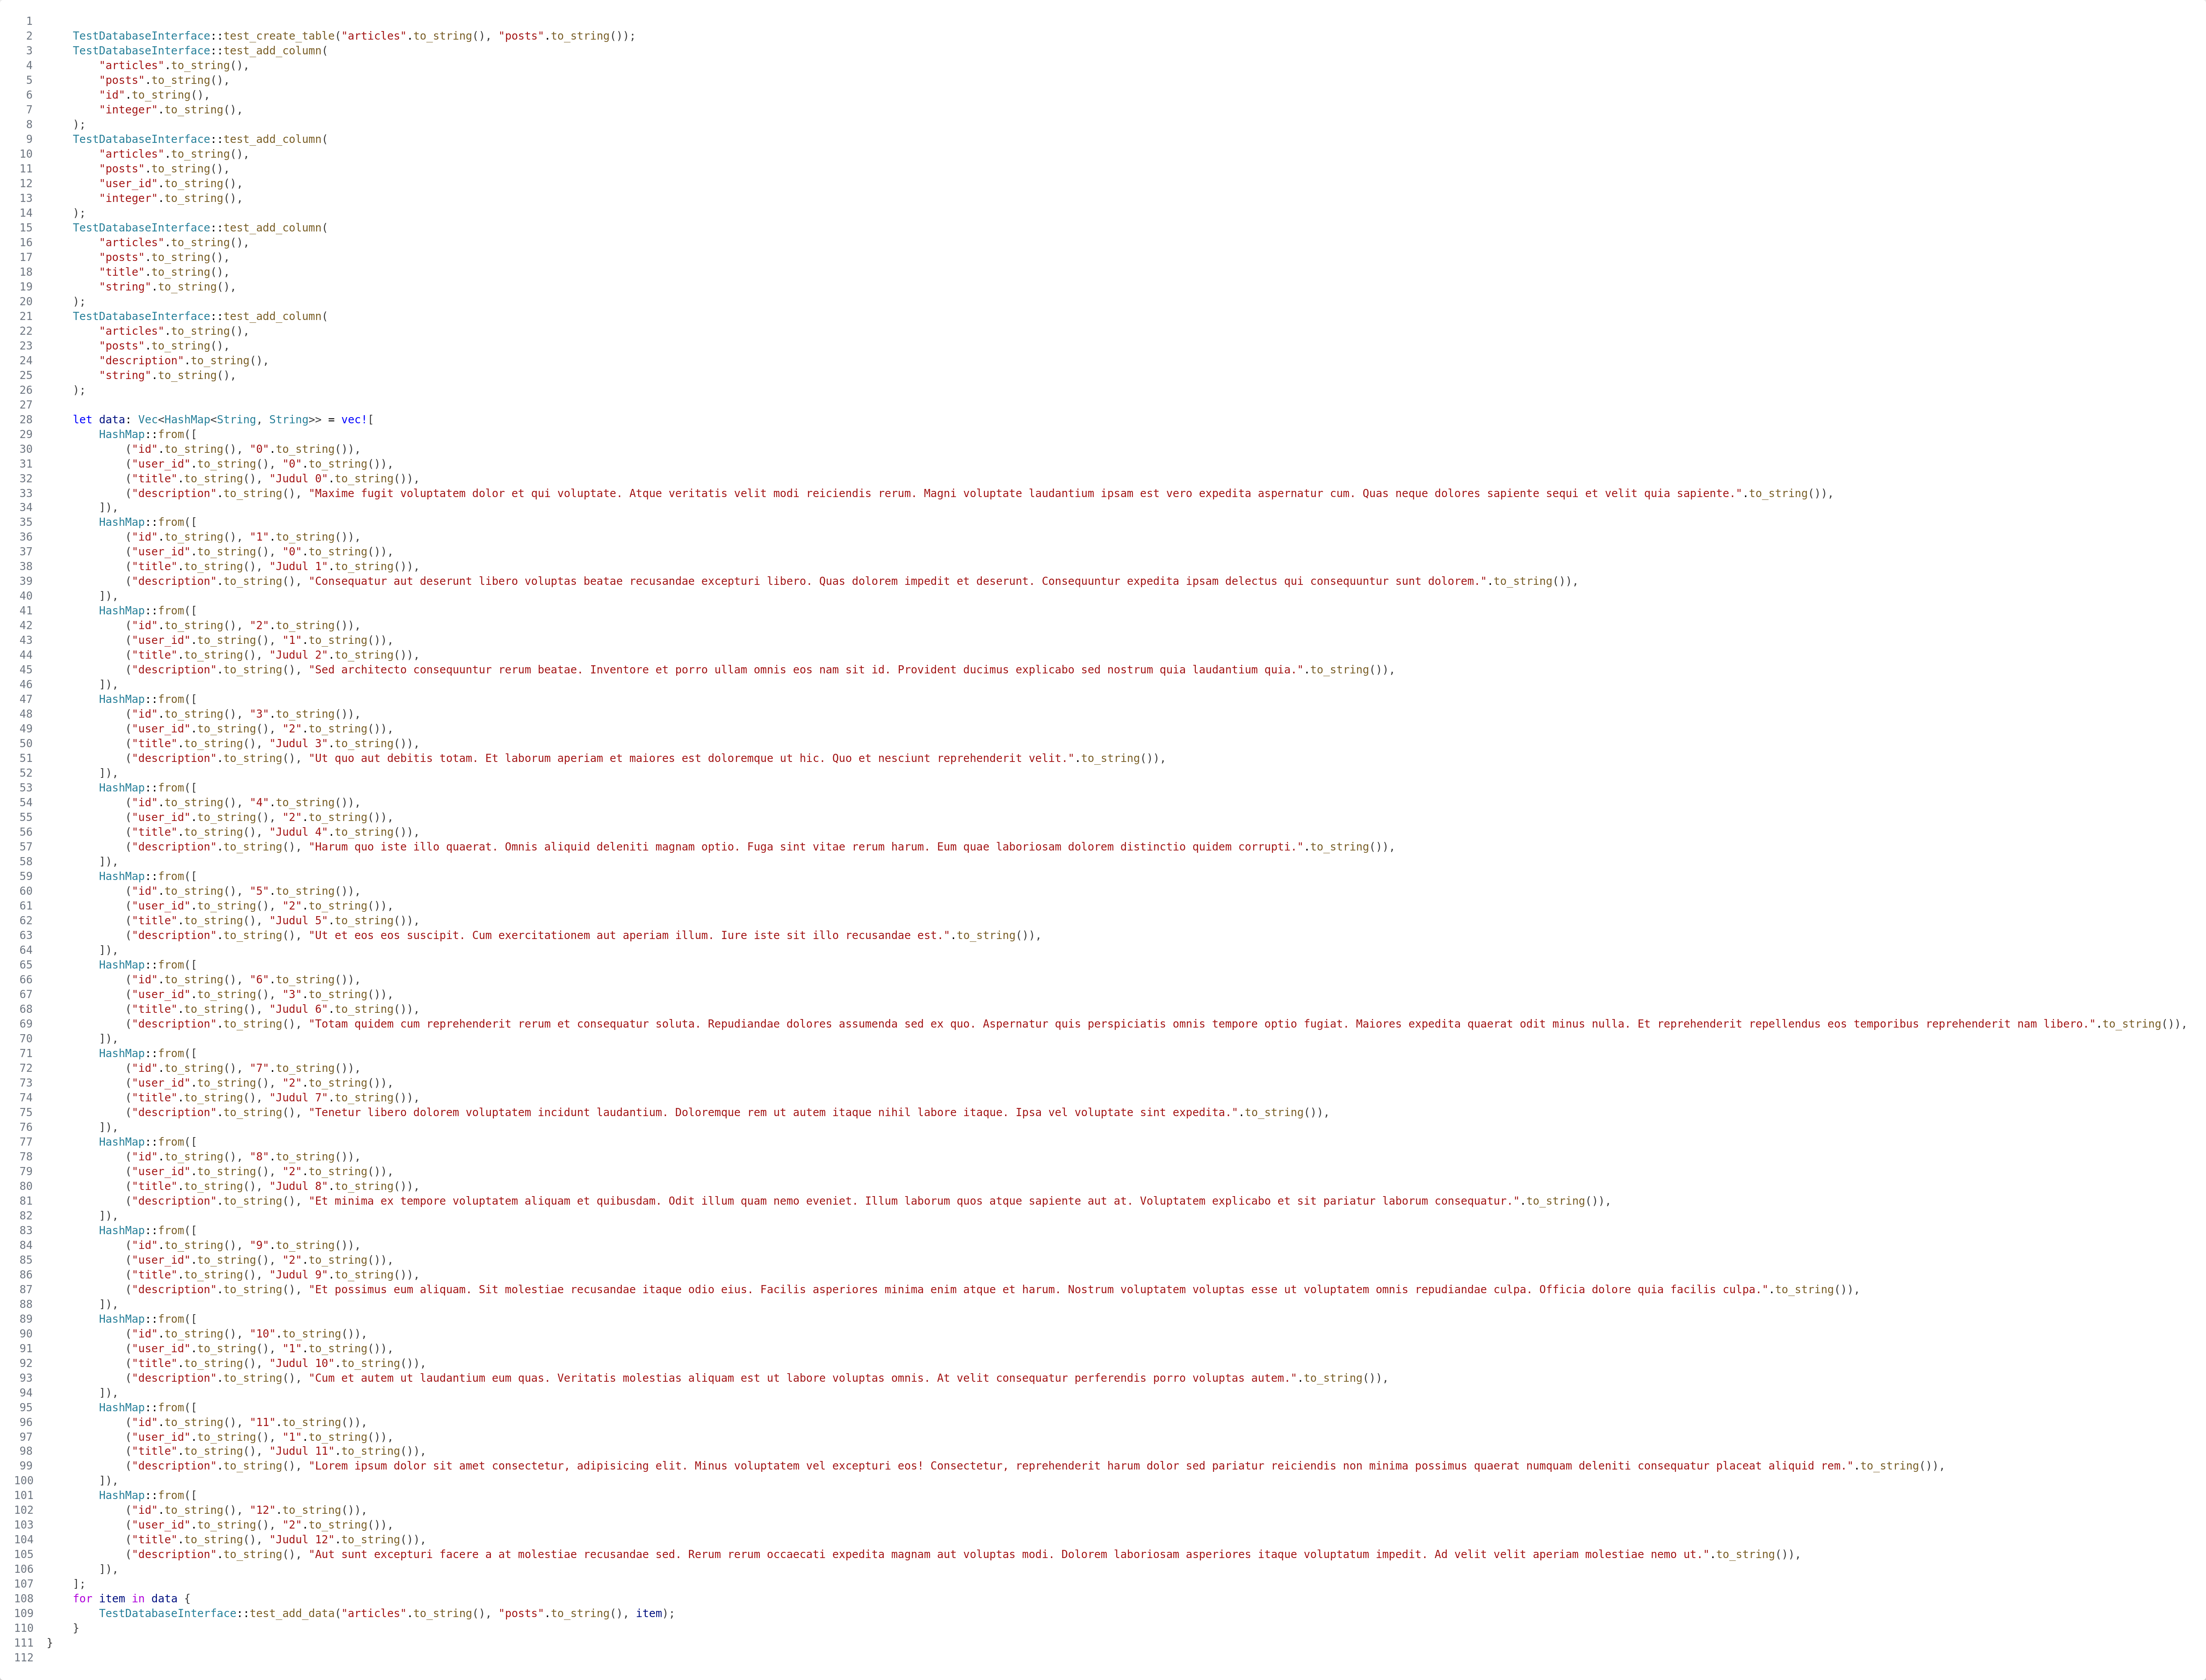
\includegraphics[width=0.6\textwidth]{gambar/lampiran/file-test-database-interface-6.png}
  \caption{\emph{File} test\_interface.rs bagian 6}
\end{figure}

\begin{figure}[H]
  \centering{}
	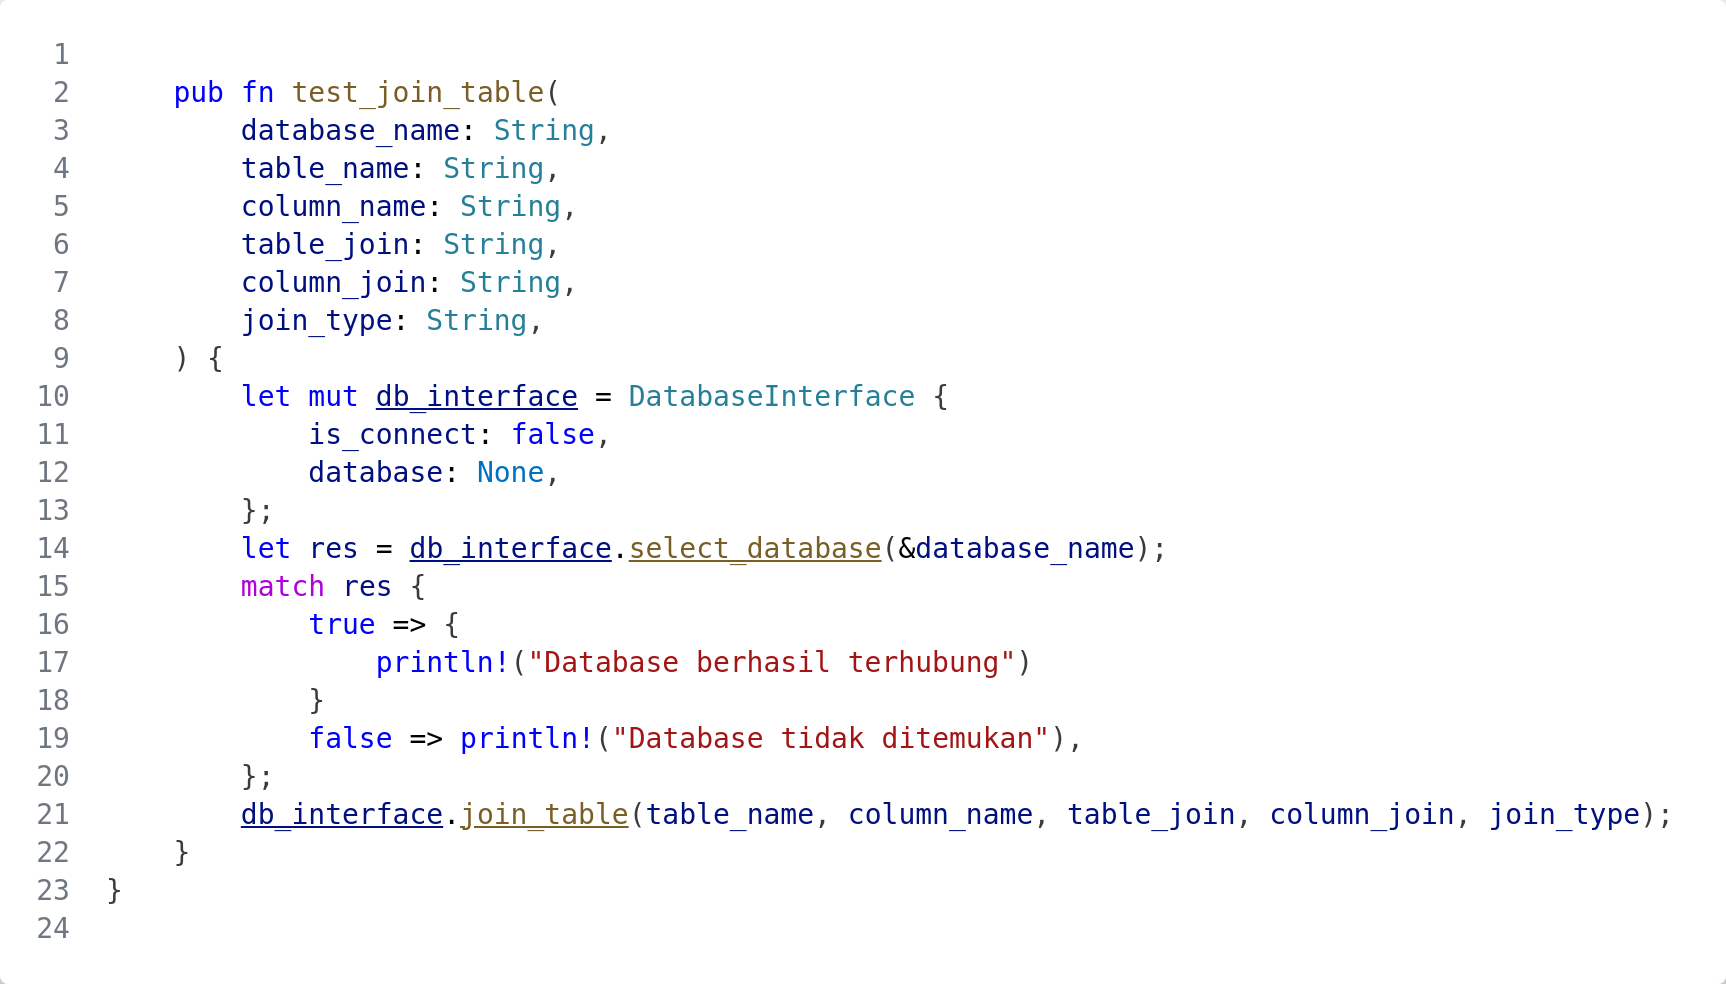
\includegraphics[width=0.6\textwidth]{gambar/lampiran/file-test-database-interface-7.png}
  \caption{\emph{File} test\_interface.rs bagian 7}
\end{figure}

\begin{figure}[H]
  \centering{}
	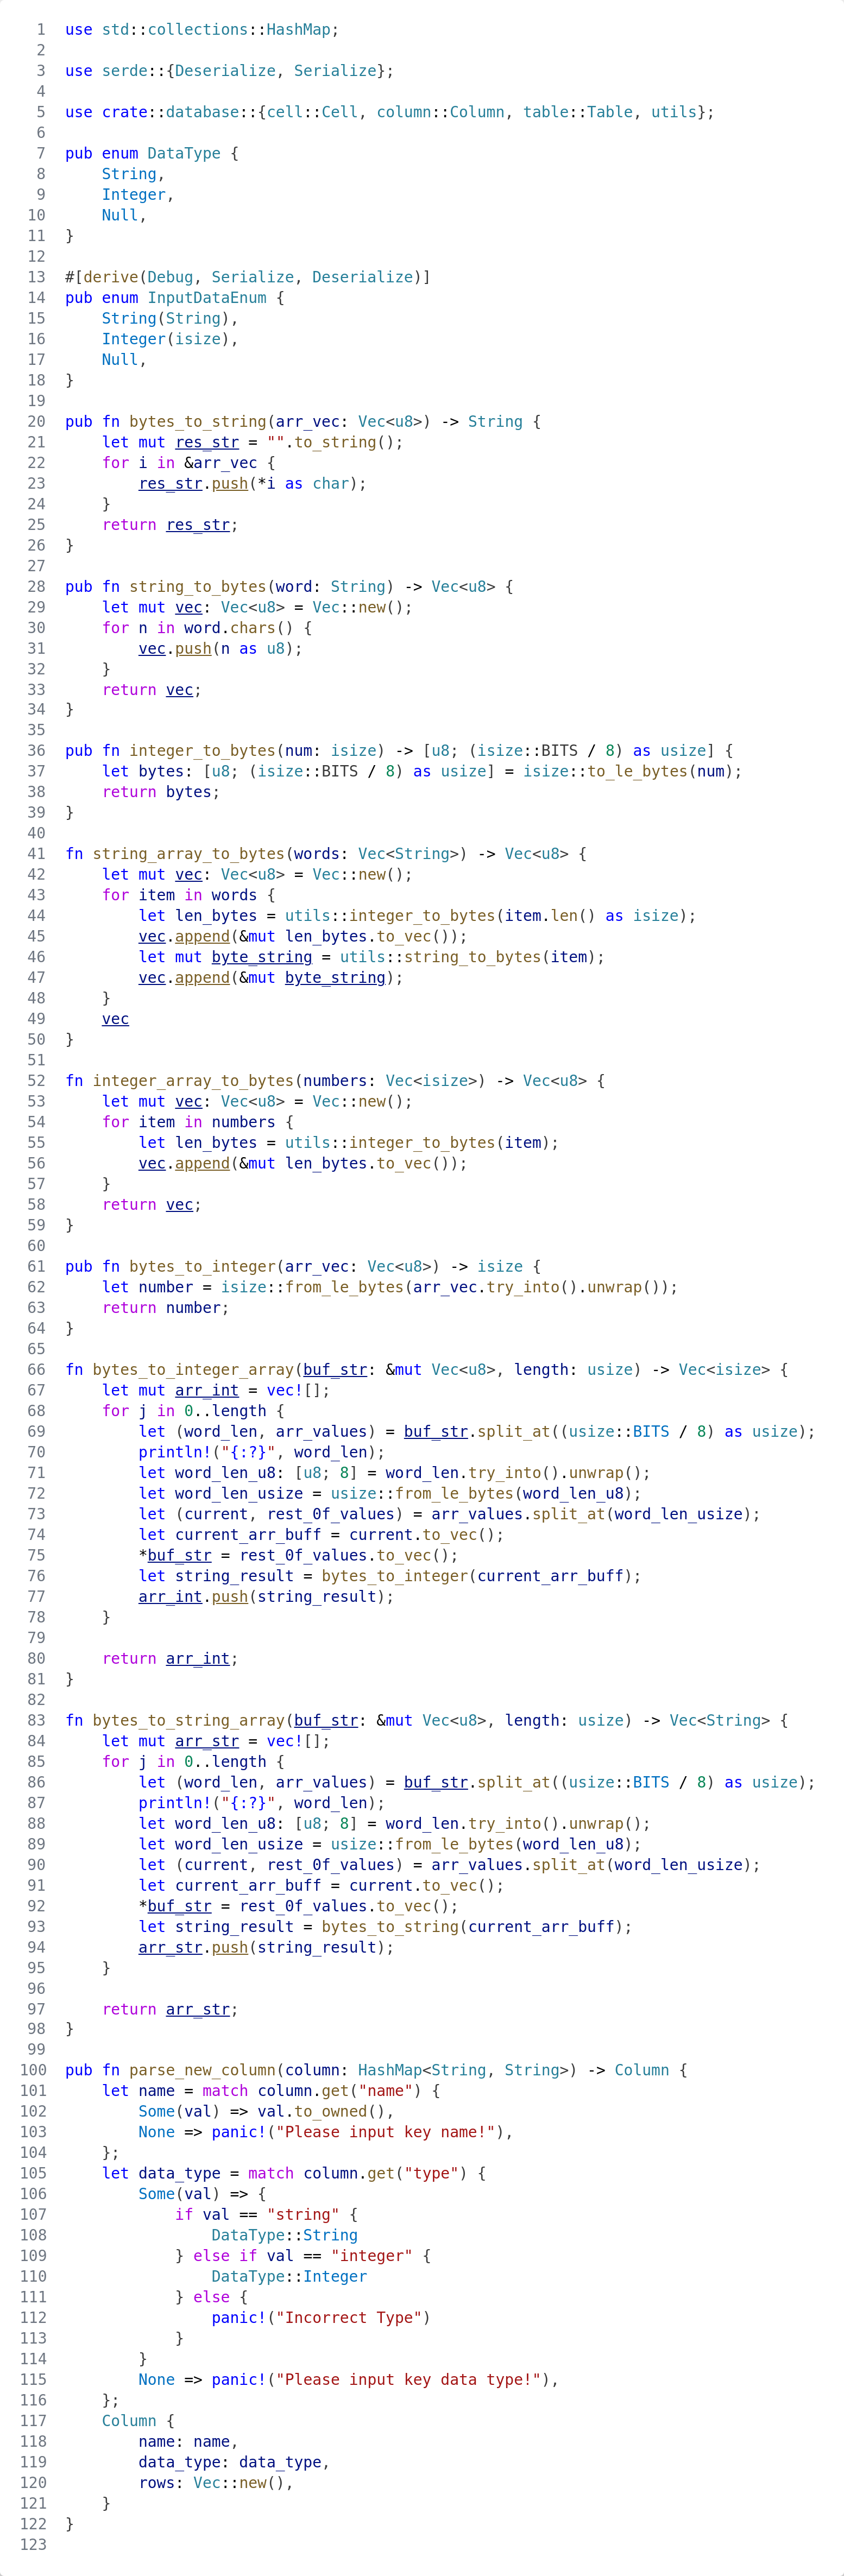
\includegraphics[width=0.4\textwidth]{gambar/lampiran/file-utils.png}
  \caption{\emph{File} utils.rs}
\end{figure}
